\chapter{Програмни конструкции}

Компютърните програми са съставени от стриктна последователност инструкции. Такива последователности се наричат алгоритъм. Ние хората всеки ден изпълняваме различни алгоритми, като част от нашето ежедневие. Да се приготвим и да отидем на училище е един алгоритъм. Събуждаме се, ставаме, обличаме се, правим си сутрешния тоалет, закусваме, излизаме от вкъщи, придвижваме се до училище. Много ярък пример за алгоритъм са рецептите за готвене. В една рецепта има начални продукти, след това точни инструкции как продуктите са се обработят и смесят, като има ясна представа какъв трябва да бъде крайният резултат. При компютърните програми има основен набор от инструкции, които съставляват изразните средства на съответния програмен език. Чарът на блоковите езици е, че този основен набор от инструкции е представен визуално, под формата на цветни блокчета. Подредбата на цветните блокчета в строго определена последователност води до създаването на малки компютърни програми. 

В случая на Scratch, програмата има ясно определена стартова точка и ясно определена финална точка. При App Inventor подходът е малко по-различен. Там последователността от инструкции, съставляващи писаната програма, се въвежда в малки фрагменти, наречени събития. Събитията възникват при различни действия от страна на потребителя или операционната система. При Scratch говорим за последователно програмиране, а при App Inventor говорим за събитийно програмиране. Основните програмни конструкции в двете програмни среди до голяма степен са идентични, но има и някои съществени разлики. За да можем да пишем ефективни и надеждни програми е важно добре да познаваме изразните средства на програмните среди с които работим. 

\section{Изразни средства в Scratch}

Базовите градивни блокчета в Scratch са организирани в цветни групи (Фиг. \ref{fig0051}). Тази организация помага за по-бързо ориентиране и по-ефективна употреба на различните блокчета. 

\begin{figure}[H]
  \centering
  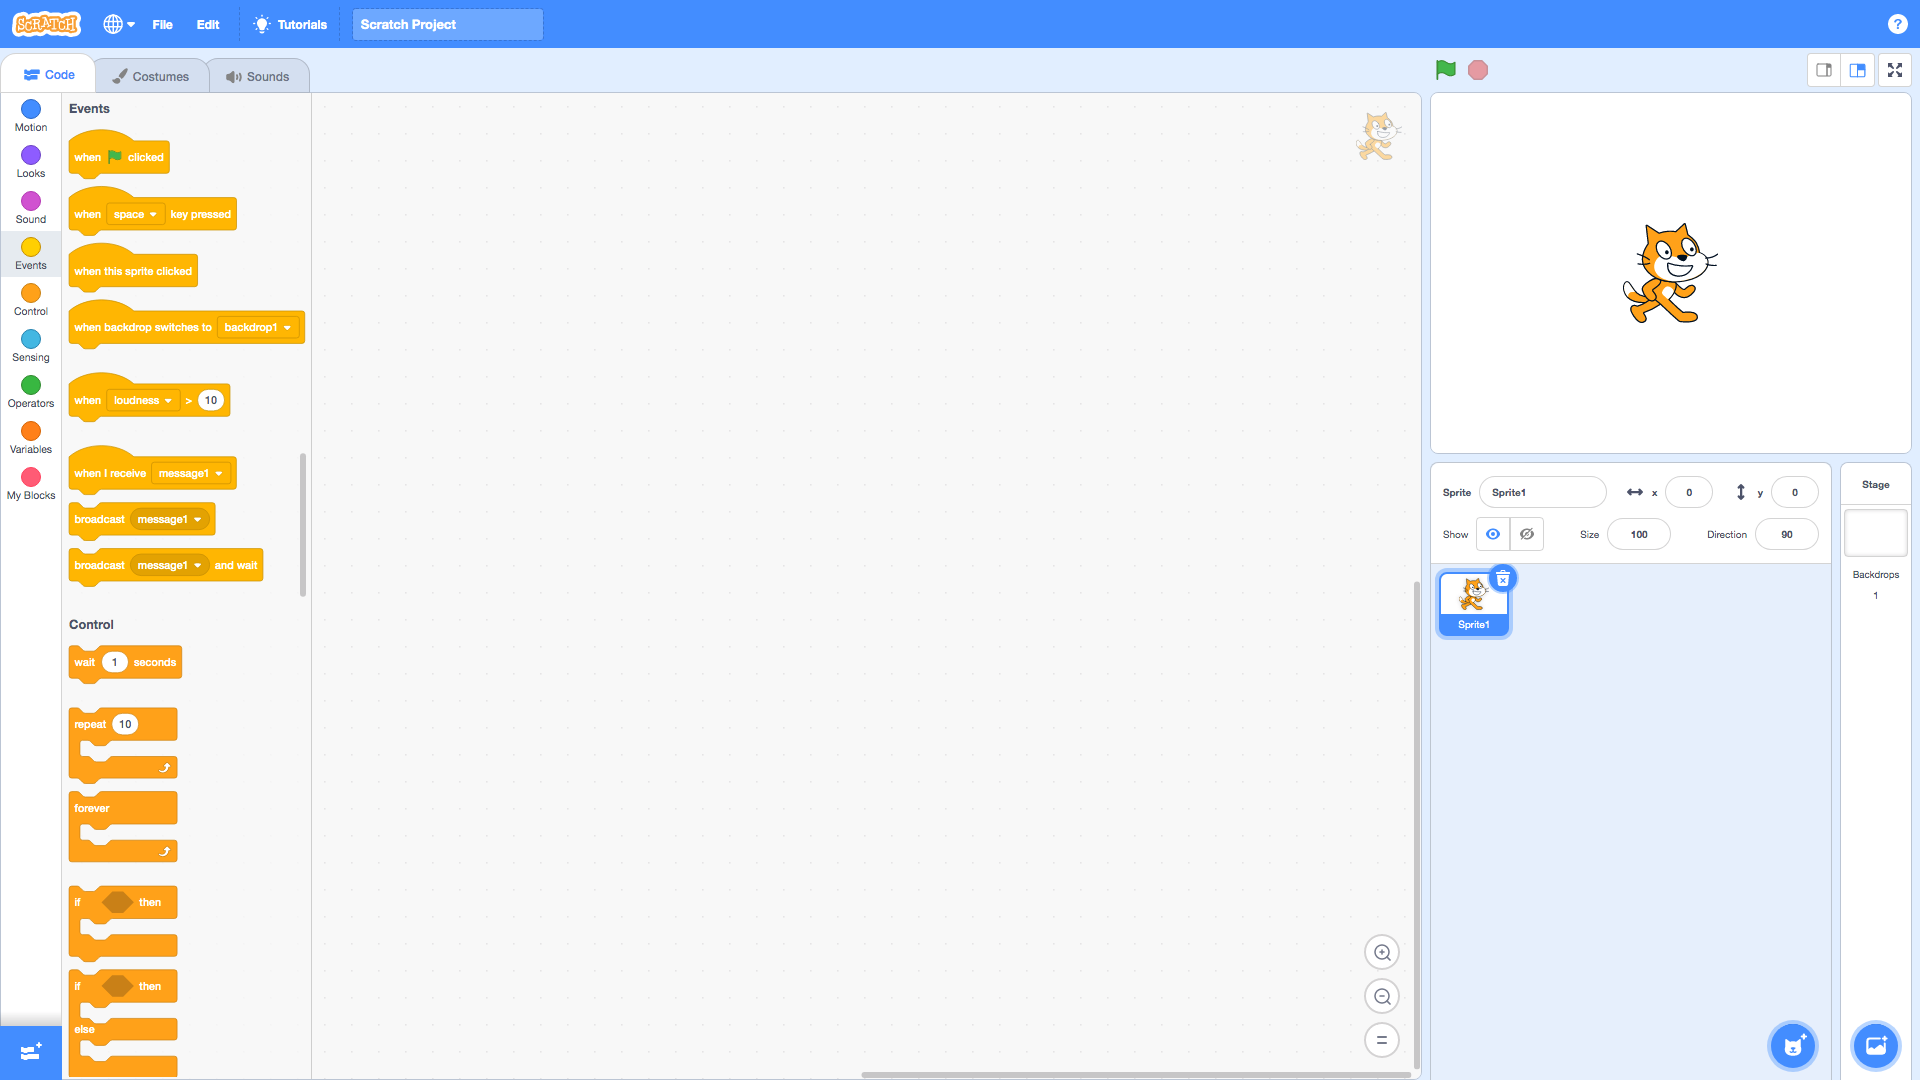
\includegraphics[width=1.0\linewidth,height=0.5\linewidth]{fig0051.png}
  \caption{Групиране на инструкциите}
\label{fig0051}
\end{figure}

Най-важното блокче в програмата е блокчето, което дава старт за изпълнение на инструкциите, които са подредени под него. Това блокче има зелен флаг (Фиг. \ref{fig0052}) и определя какво ще последва след стартирането на програмата.

\begin{figure}[H]
  \centering
  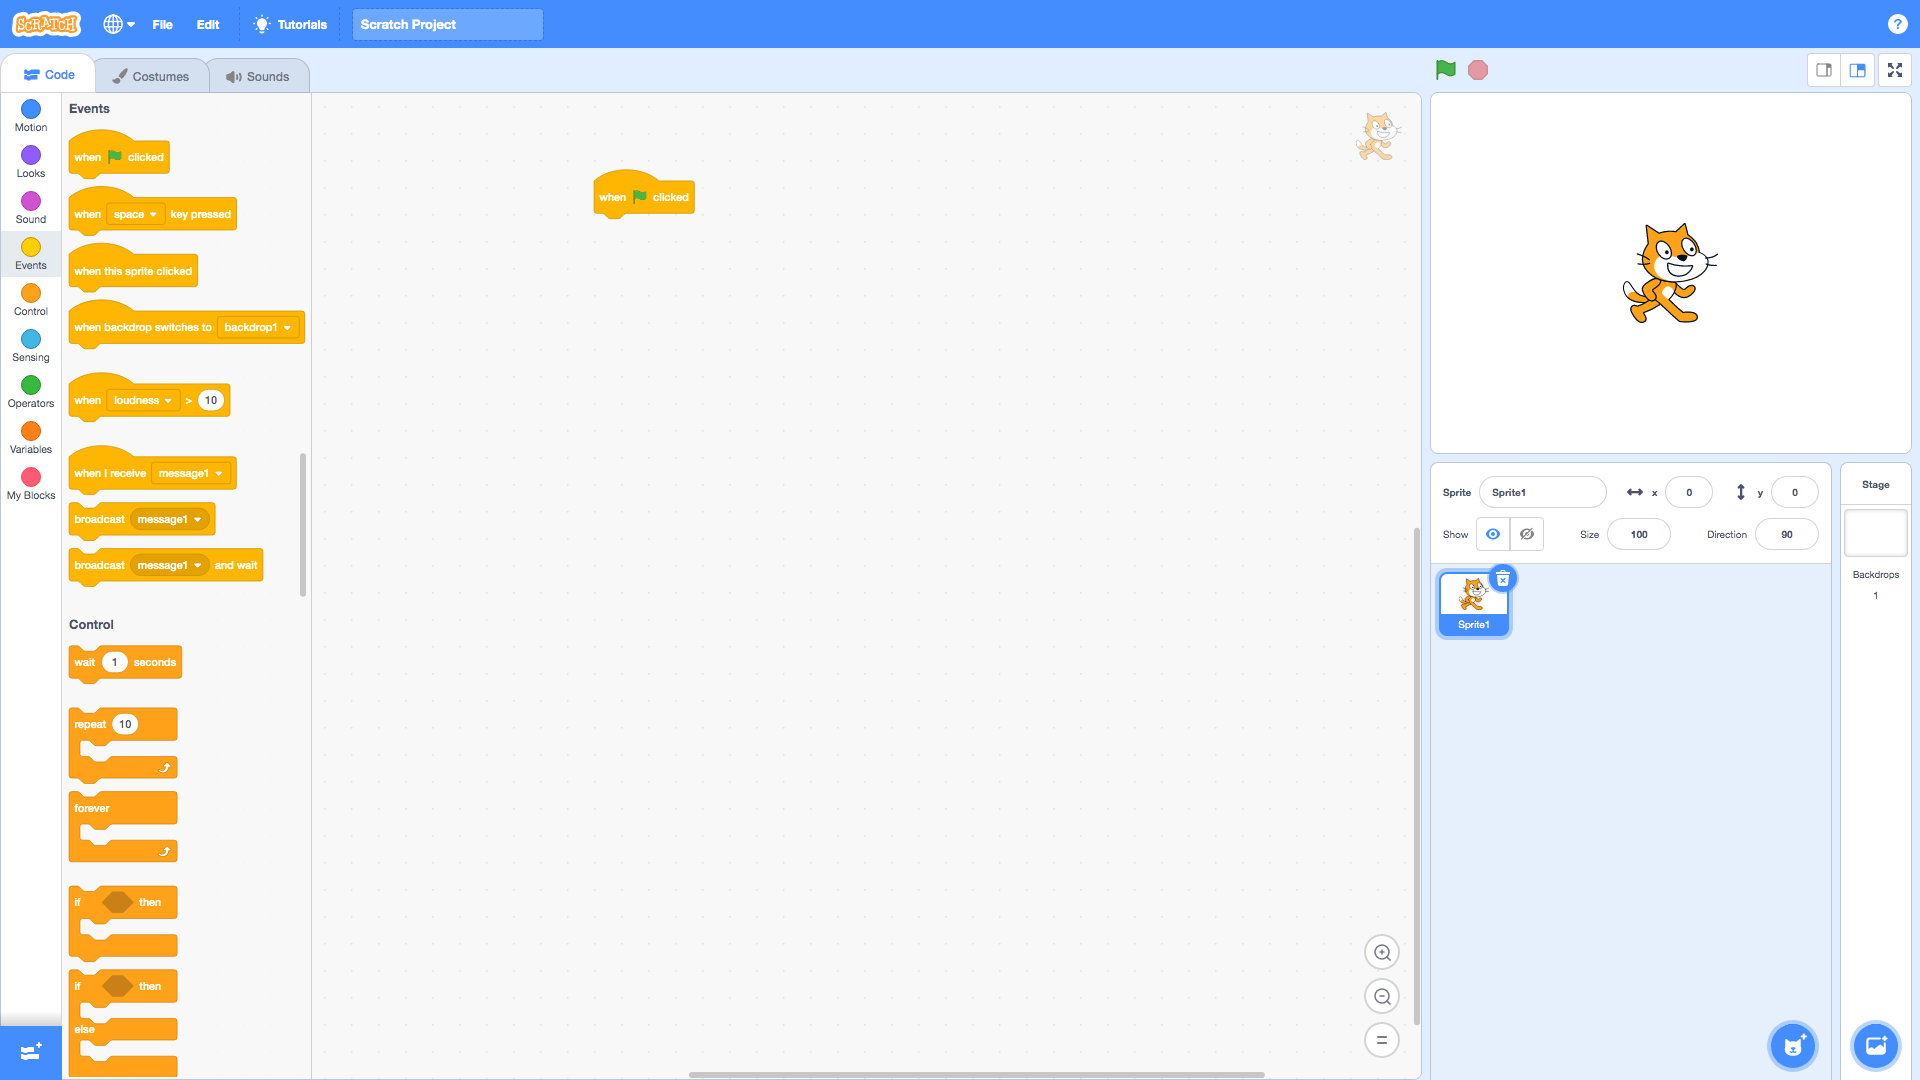
\includegraphics[width=1.0\linewidth,height=0.5\linewidth]{fig0052.png}
  \caption{Начална точка на програмата}
\label{fig0052}
\end{figure}

Блокчето за старт на програмата се намира в светло оранжевата група, която е предназначена да реагира на събития от страна на потребителя. Точният момент в който потребителят иска програмата да започне своето изпълнение е неопределен във времето и поради тази причина Scratch трябва да улови събитие, предизвикано от самия потребител. 

Второто по важност блокче служи за край на програмата (Фиг. \ref{fig0053}). То се намира в тъмно оранжевата група и има за задача да спре всички процеси, извършващи се по време на изпълнението на самата програма.

\begin{figure}[H]
  \centering
  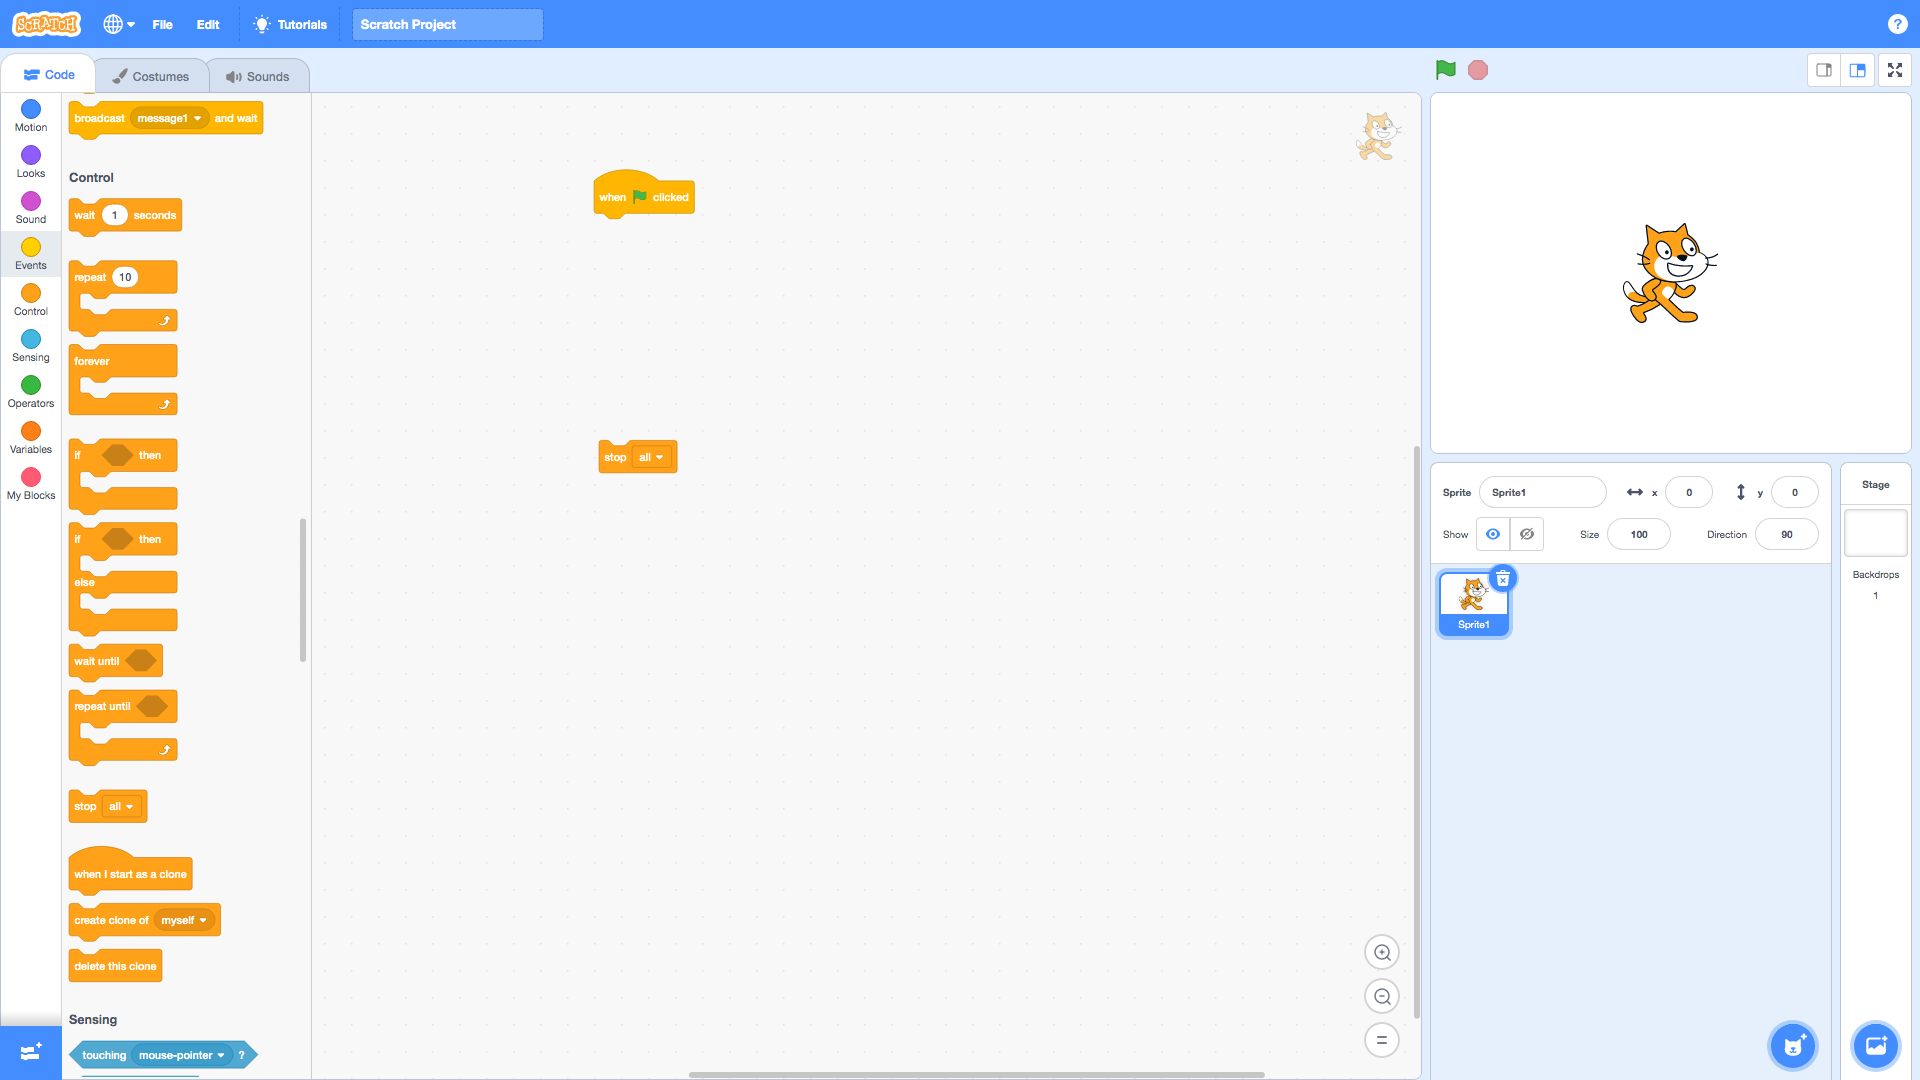
\includegraphics[width=1.0\linewidth,height=0.5\linewidth]{fig0053.png}
  \caption{Крайна точка на програмата}
\label{fig0053}
\end{figure}

Тъмно оранжевата група съдържа блокчета за контрол на изпълнението. Тези блокчета позволяват програмата да поема по различни пътища, както и група от действия да се повтарят многократно. 

В Scratch блокчетата инструкции основно контролират картинки, наречени спрайтове (sprites). За разлика от обикновеното компютърно изображение, спрайтът е графичен обект, който съдържа множество кадри, показващи изображението на героя в различни конфигурации. Всяка нова програма в Scratch започва с един спрайт, на оранжевата котка, разположена на координати (x=0,y=0). Работното пространство е двуизмерна координатна система с център (0,0). 

\begin{figure}[H]
  \centering
  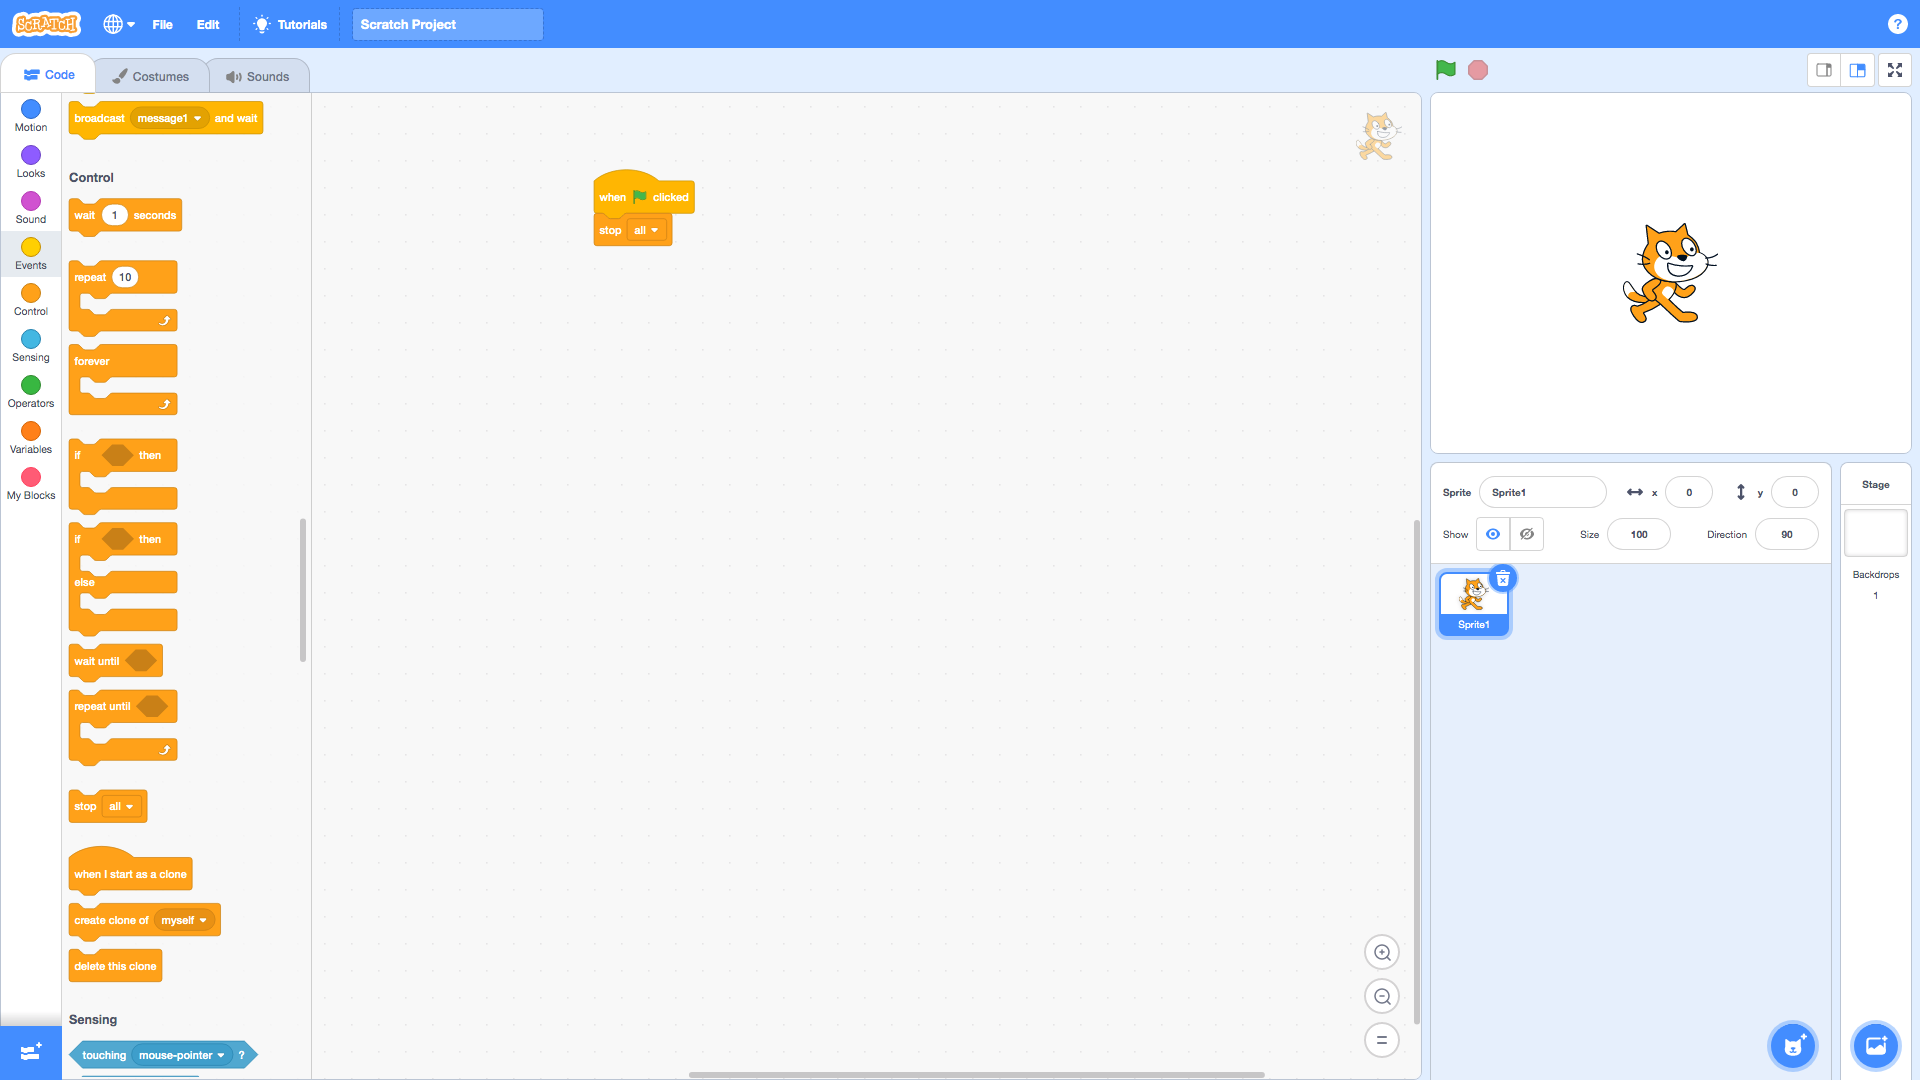
\includegraphics[width=1.0\linewidth,height=0.5\linewidth]{fig0054.png}
  \caption{Завършване веднага след започване}
\label{fig0054}
\end{figure}

Ако бъдат съединени, блокчетата за начало и за край (Фиг. \ref{fig0054}), то програмата не изпълнява нищо. Практически, тази програма приключва веднага след като е започнала. Програма, която не прави нищо е напълно безсмислена. За да започне нещо да се случва се използват блокчетата в синята група. Първото блокче инструктира котето да се премести 10 стъпки, като броя стъпки може да бъде променени, чрез изписване на друго число във вътрешността на блокчето (Фиг. \ref{fig0055}).

\begin{figure}[H]
  \centering
  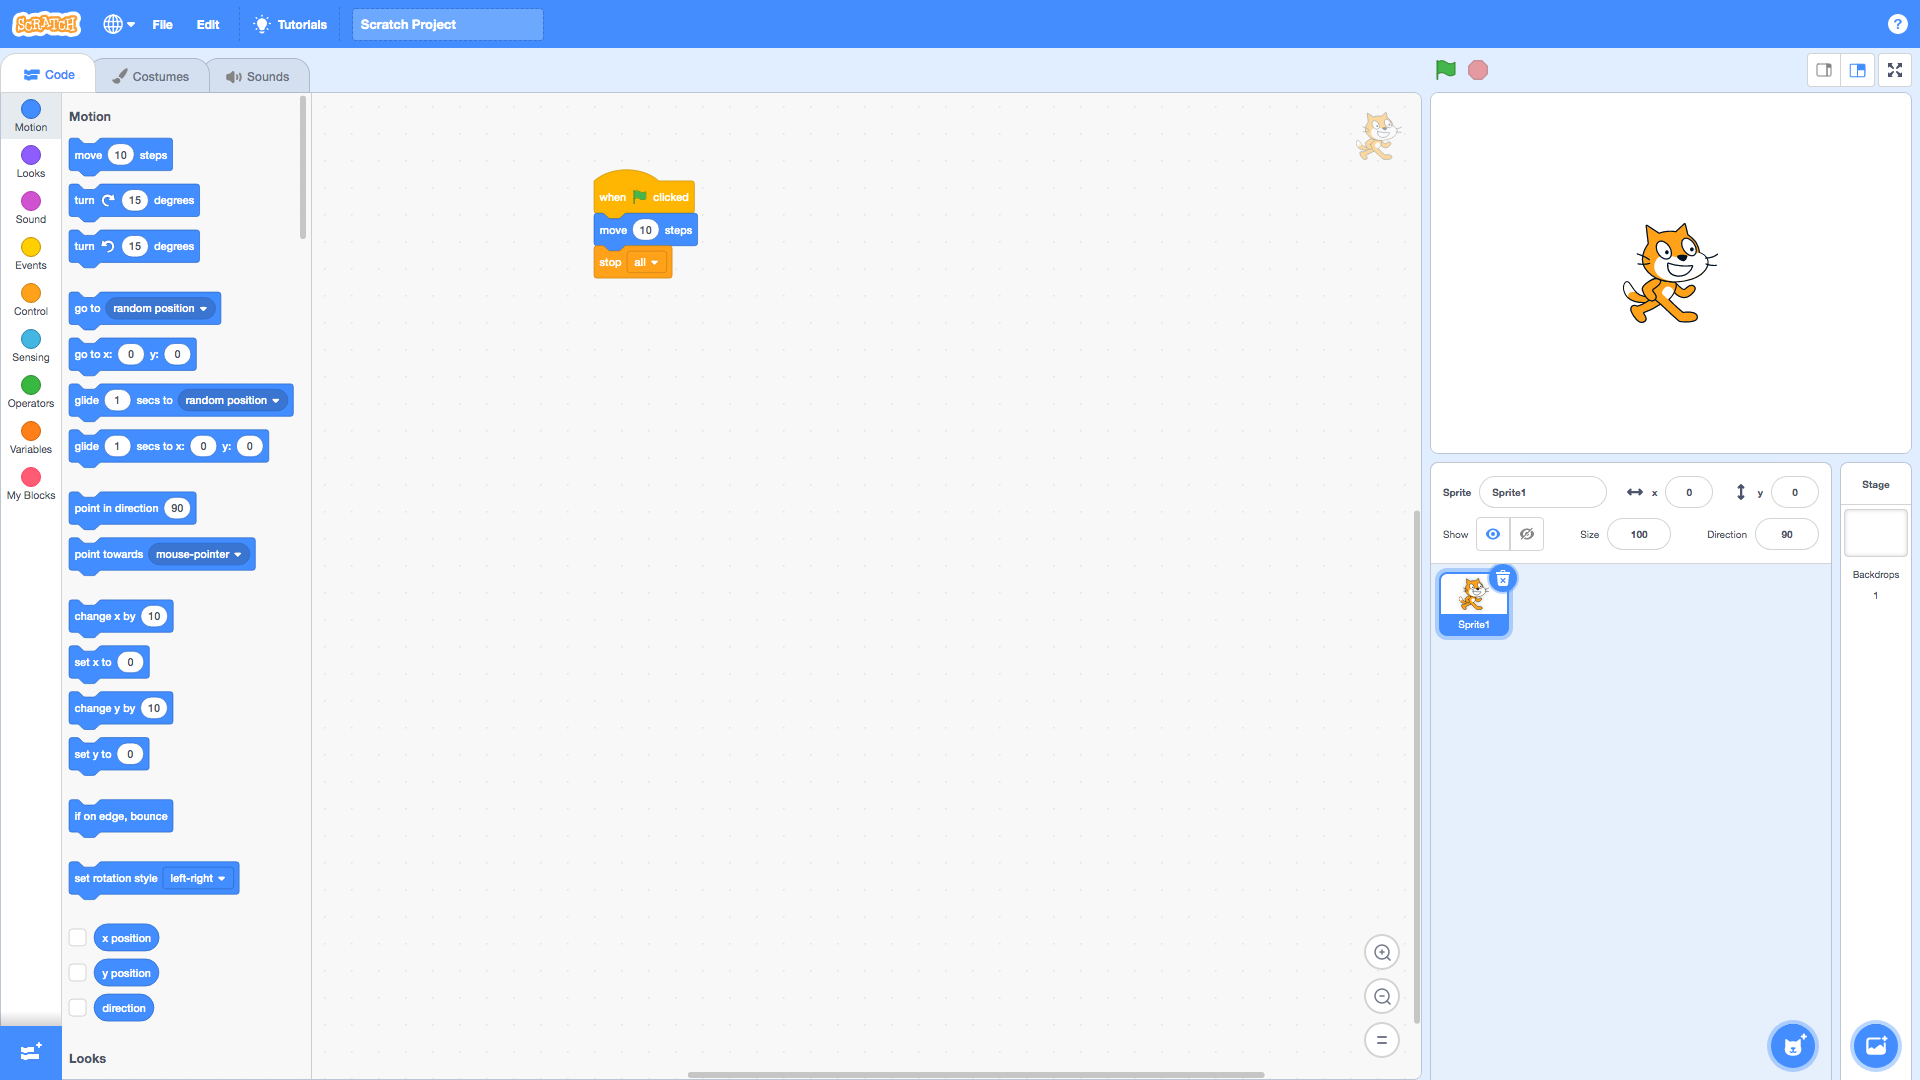
\includegraphics[width=1.0\linewidth,height=0.5\linewidth]{fig0055.png}
  \caption{Преместване на героя}
\label{fig0055}
\end{figure}

Следващият блок в групата инструктира героя да се завърти на определено число градуси, по часовниковата стрелка, спрямо собствения си център (Фиг. \ref{fig0056}).

\begin{figure}[H]
  \centering
  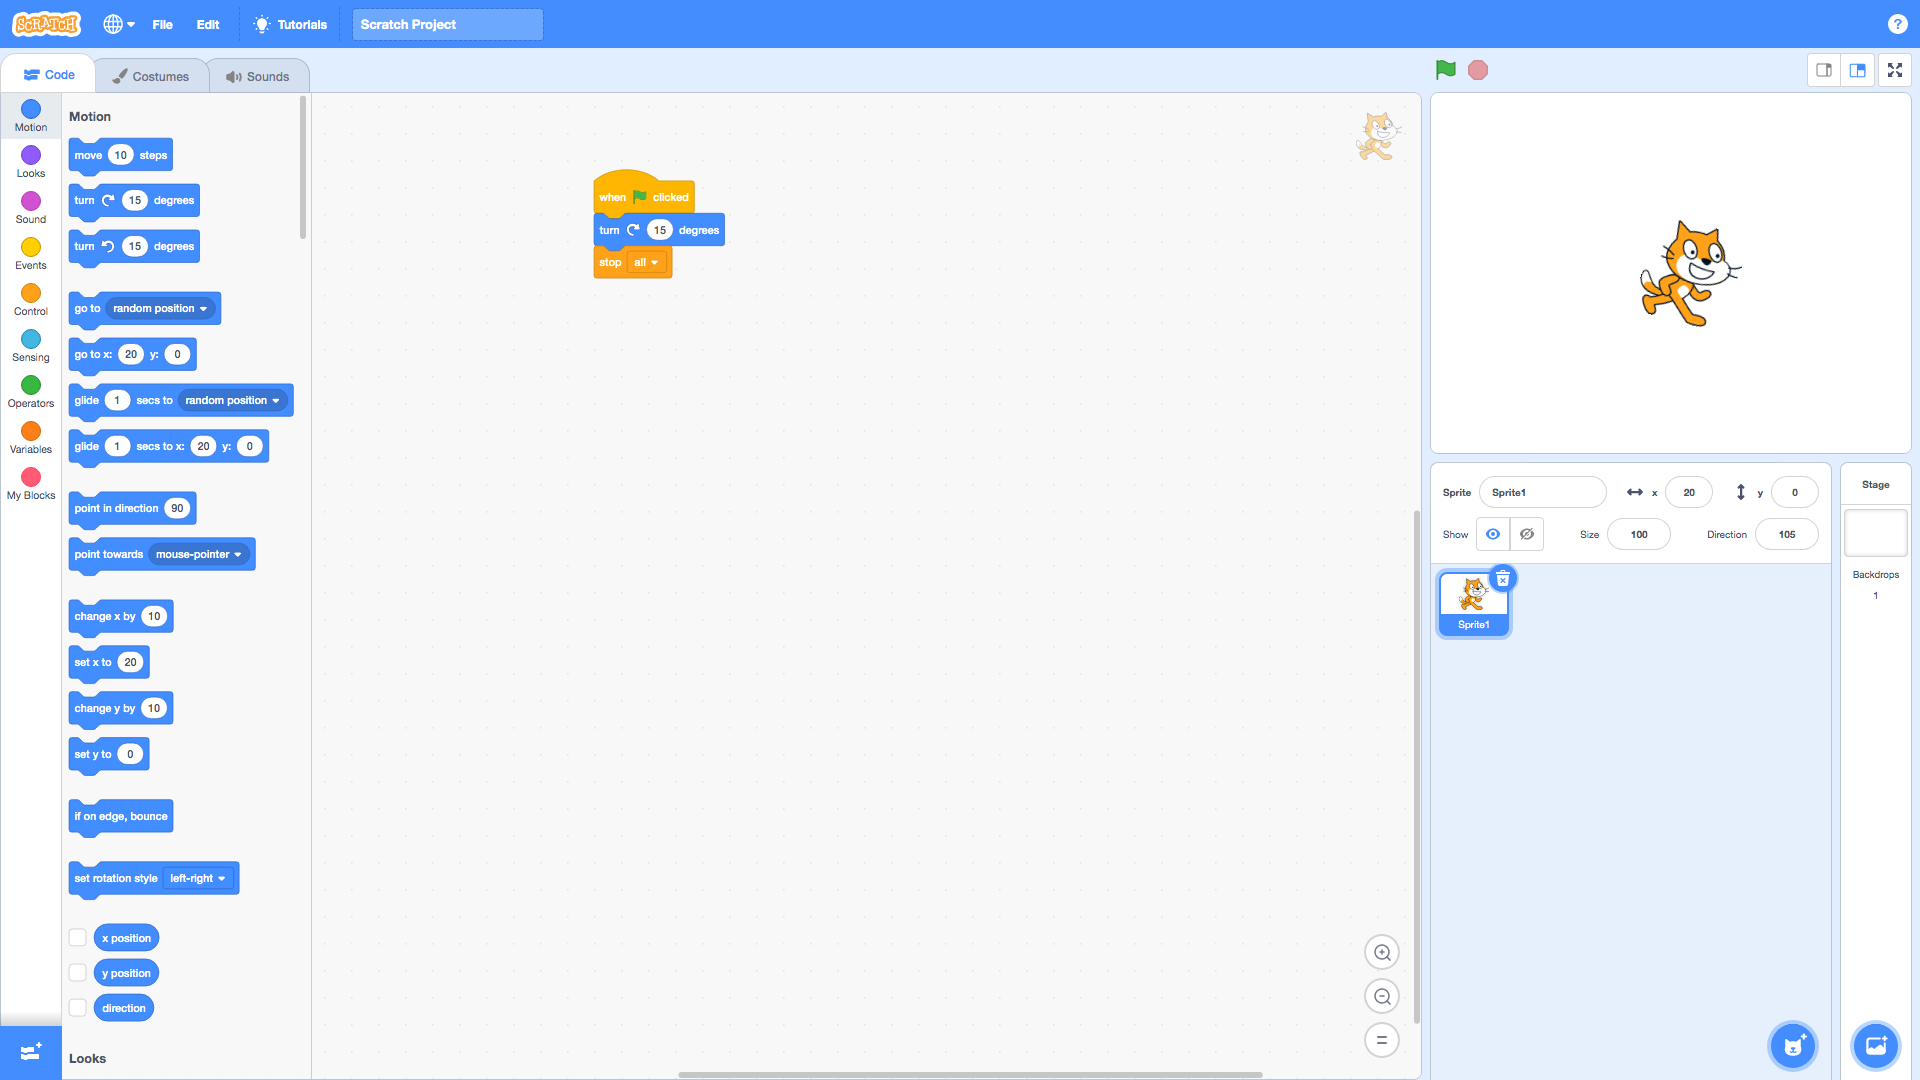
\includegraphics[width=1.0\linewidth,height=0.5\linewidth]{fig0056.png}
  \caption{Завъртане по часовниковата стрелка}
\label{fig0056}
\end{figure}

Аналогично, със следващото блокче в групата, завъртането може да се изпълни и в посока обратна на часовниковата стрелка (Фиг. \ref{fig0057}).

\begin{figure}[H]
  \centering
  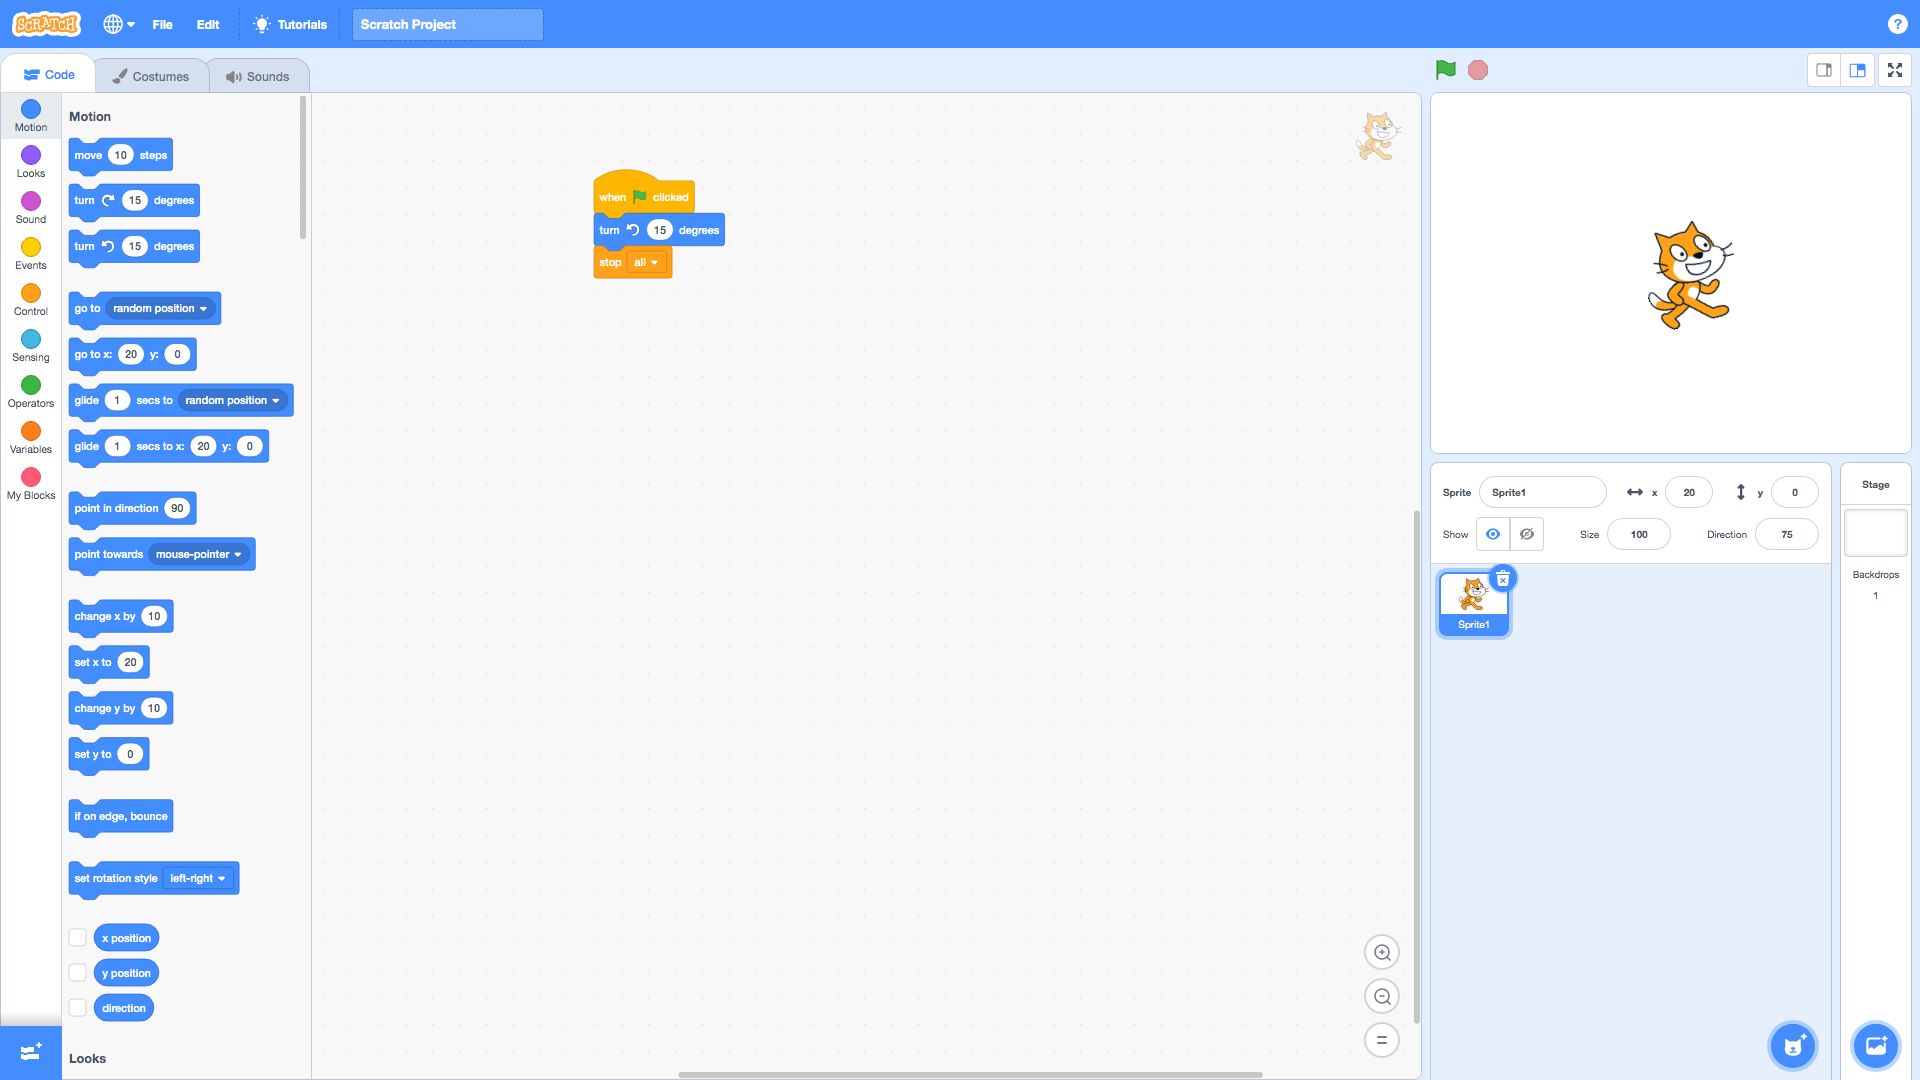
\includegraphics[width=1.0\linewidth,height=0.5\linewidth]{fig0057.png}
  \caption{Завъртане обратно на часовниковата стрелка}
\label{fig0057}
\end{figure}

Следващия блок в групата дава възможност героят да се премести на случайни координати или на координати посочени с мишката (Фиг. \ref{fig0058}).

\begin{figure}[H]
  \centering
  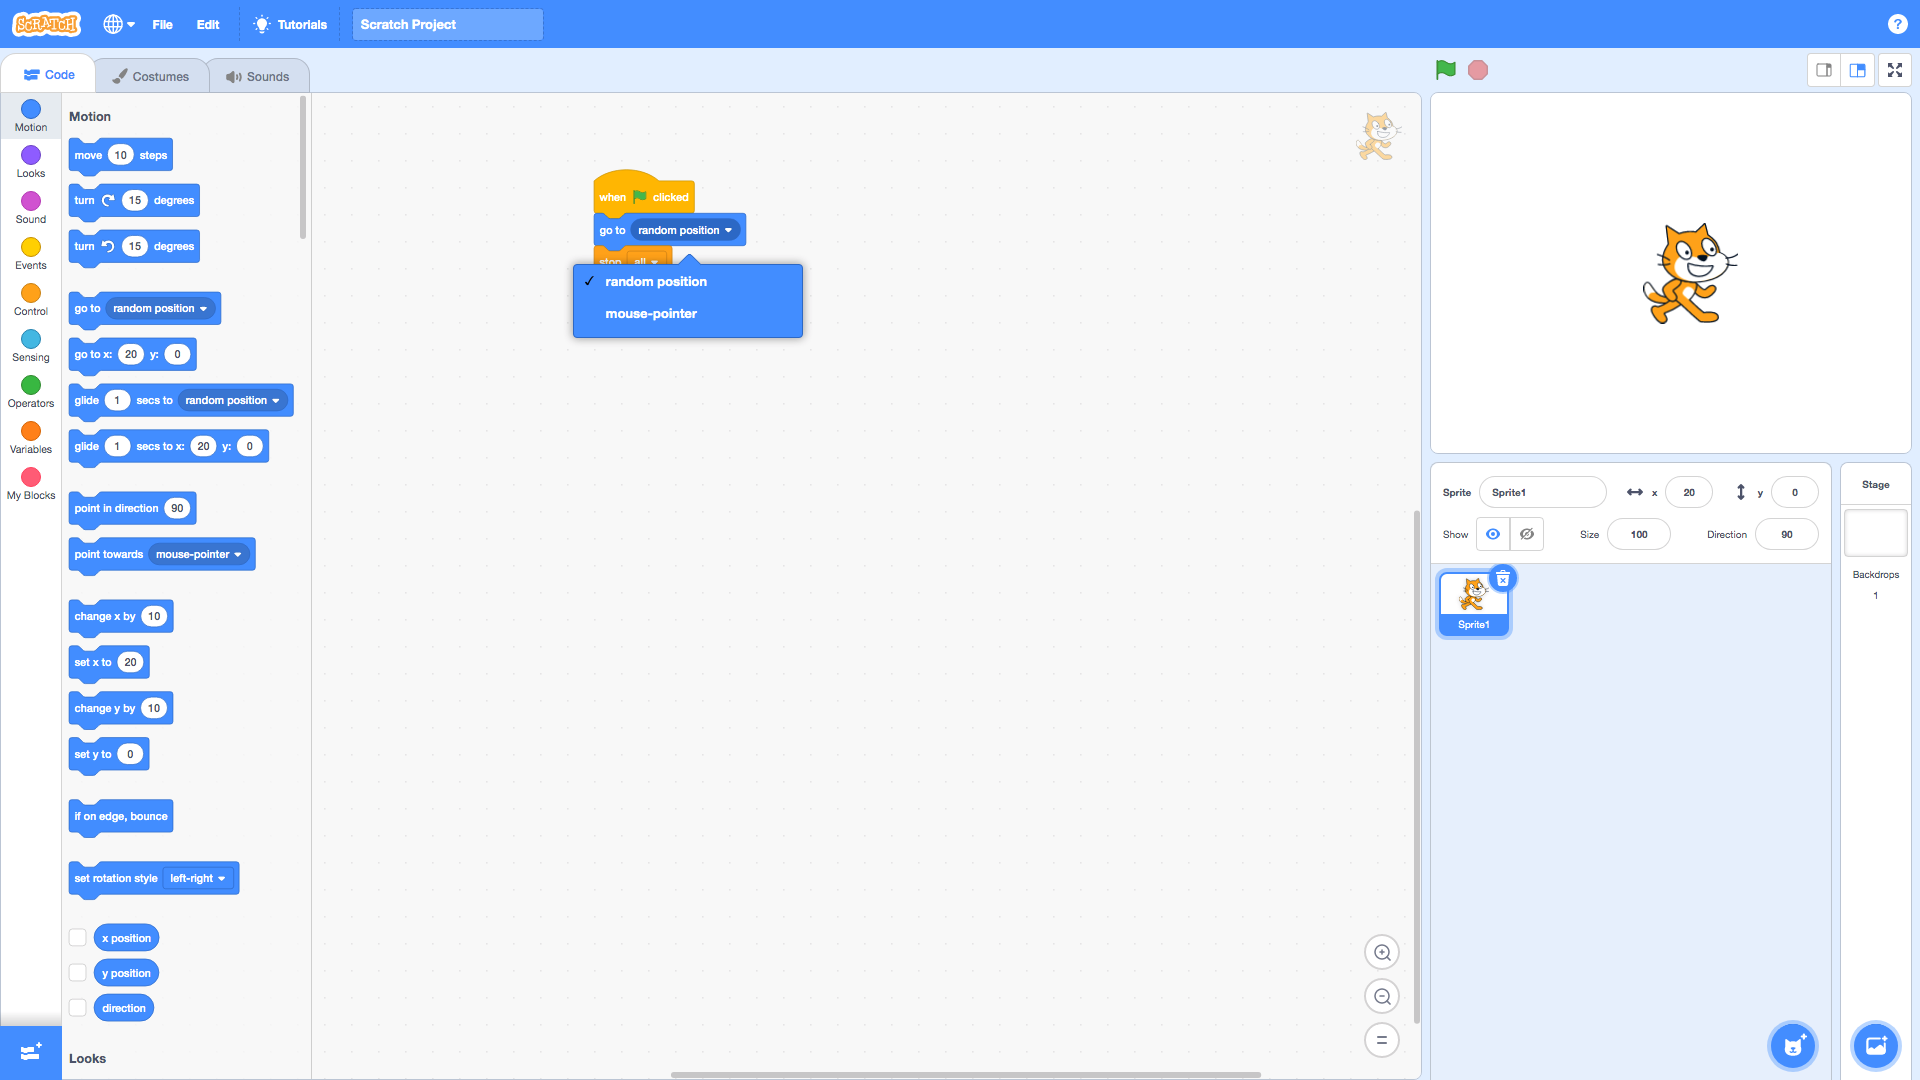
\includegraphics[width=1.0\linewidth,height=0.5\linewidth]{fig0058.png}
  \caption{Преместване на случайна позиция}
\label{fig0058}
\end{figure}

Движението на героя може да бъде зададено и чрез абсолютни координати с блокче, позволяващо да се впишат числа за абцисната и ординатната ос (Фиг. \ref{fig0059}).

\begin{figure}[H]
  \centering
  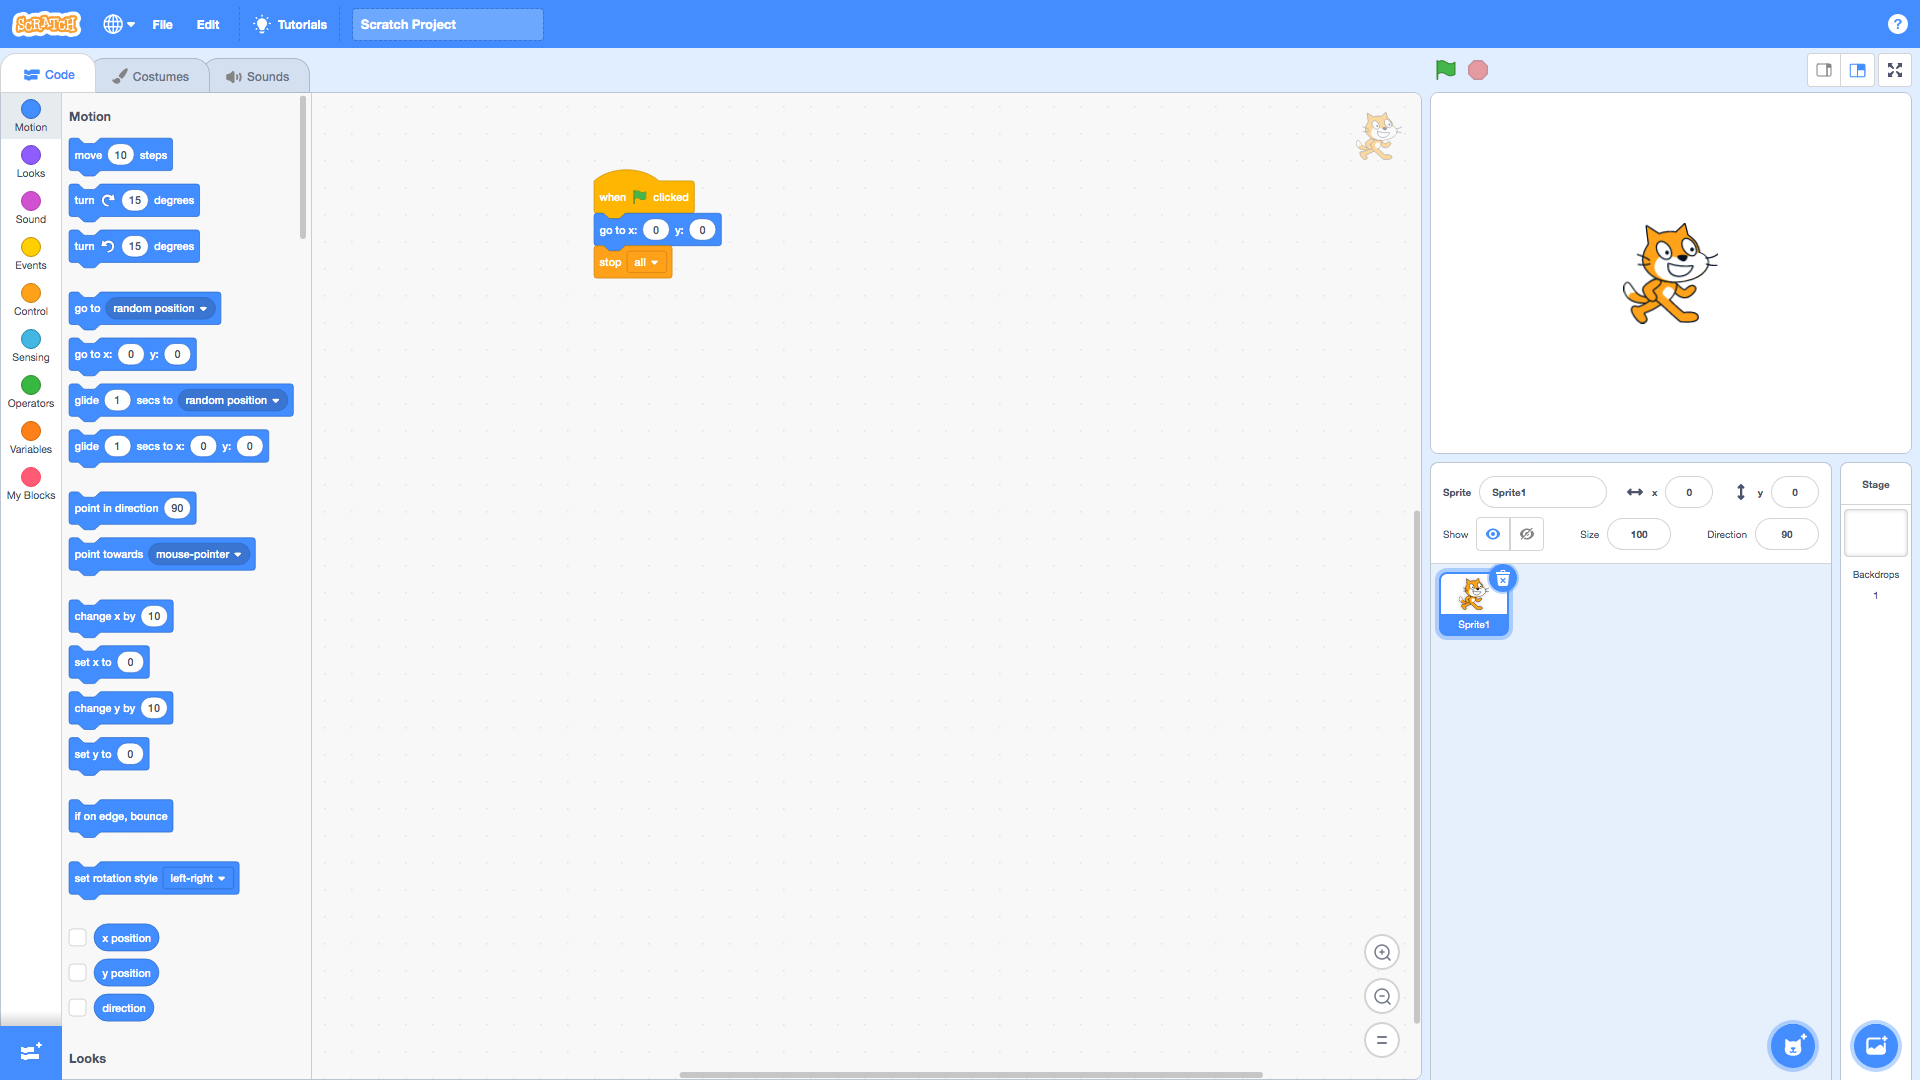
\includegraphics[width=1.0\linewidth,height=0.5\linewidth]{fig0059.png}
  \caption{Преместване по абсолютни координати}
\label{fig0059}
\end{figure}

Плавно придвижване, по предварително зададен интервал от време, е възможно на случайни координати или координати посочени с мишката, благодарение на следващото блокче в групата (Фиг. \ref{fig0060}).

\begin{figure}[H]
  \centering
  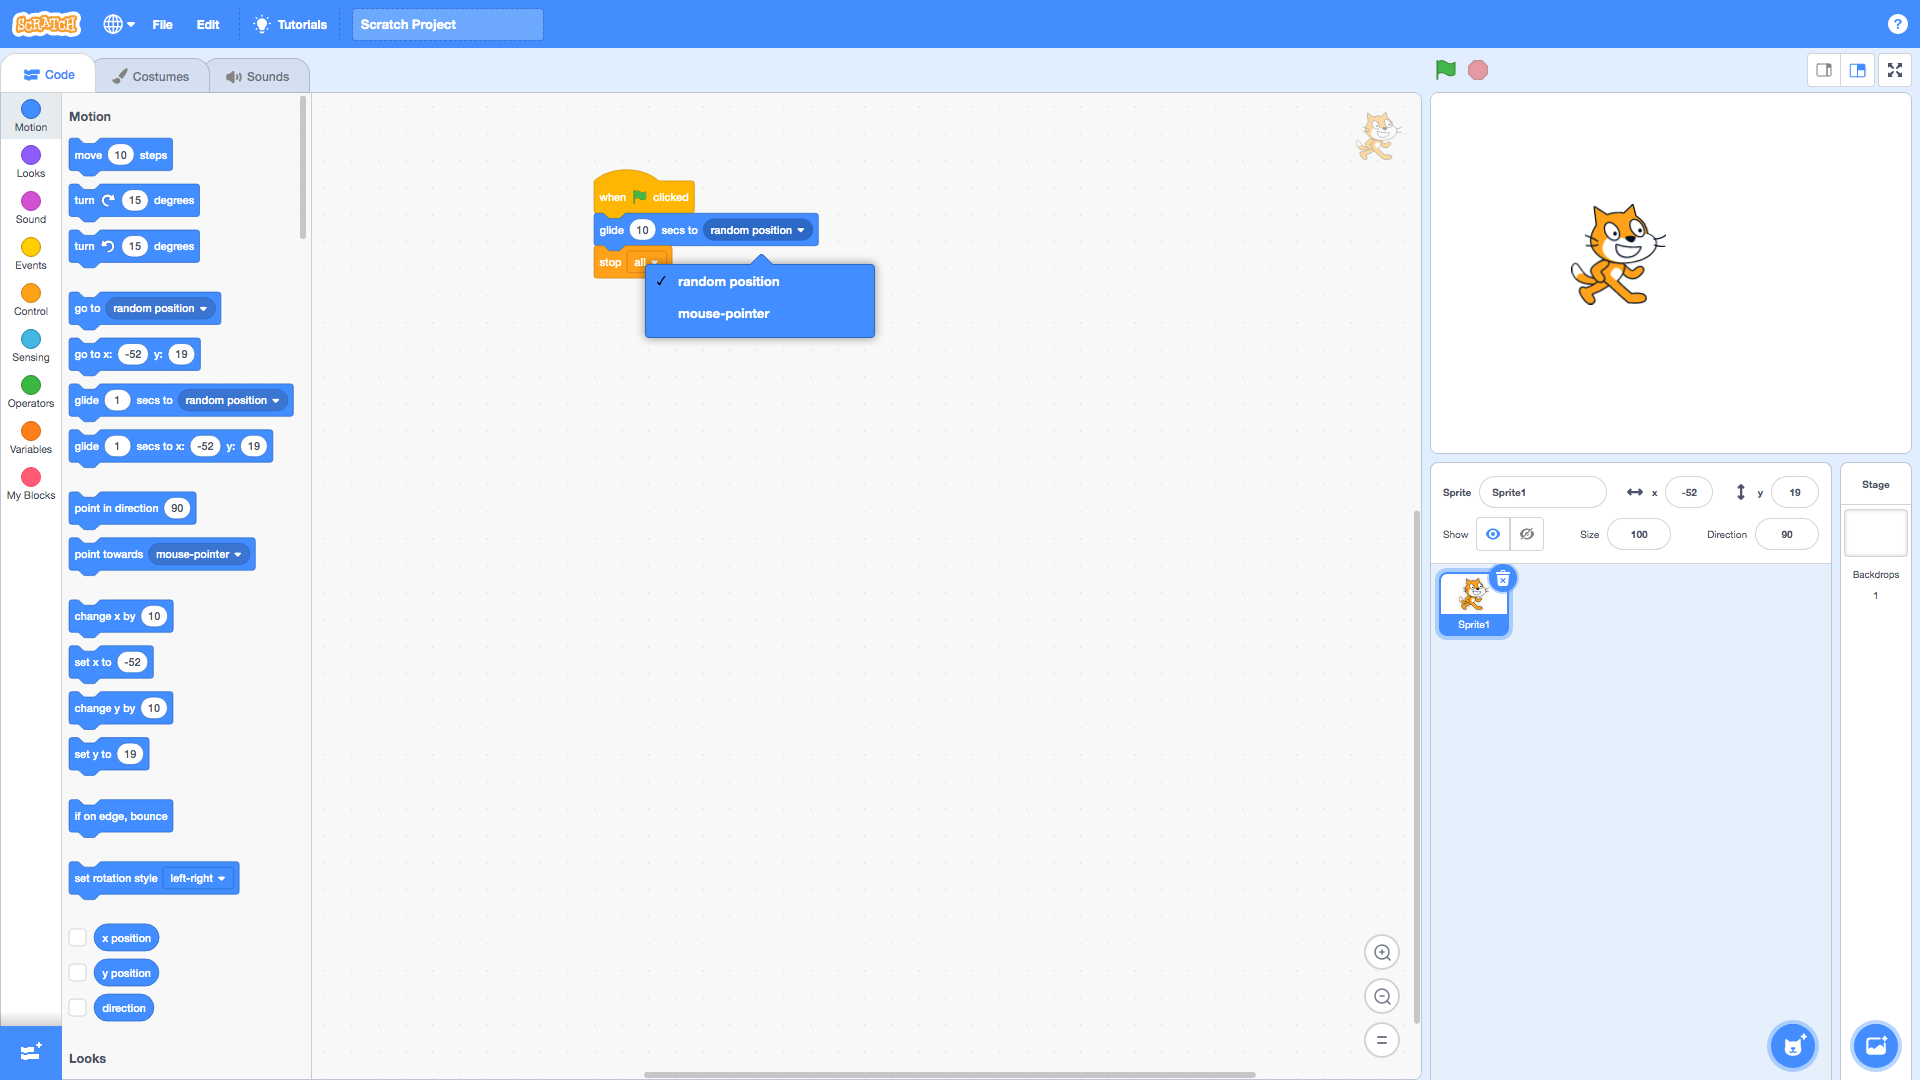
\includegraphics[width=1.0\linewidth,height=0.5\linewidth]{fig0060.png}
  \caption{Плъзгане до случайна позиция}
\label{fig0060}
\end{figure}

Плавното плъзгане до предварително зададени координати, за предварително определен интервал от време, е възможно с блокчето предназначено за тази цел (Фиг. \ref{fig0061}).

\begin{figure}[H]
  \centering
  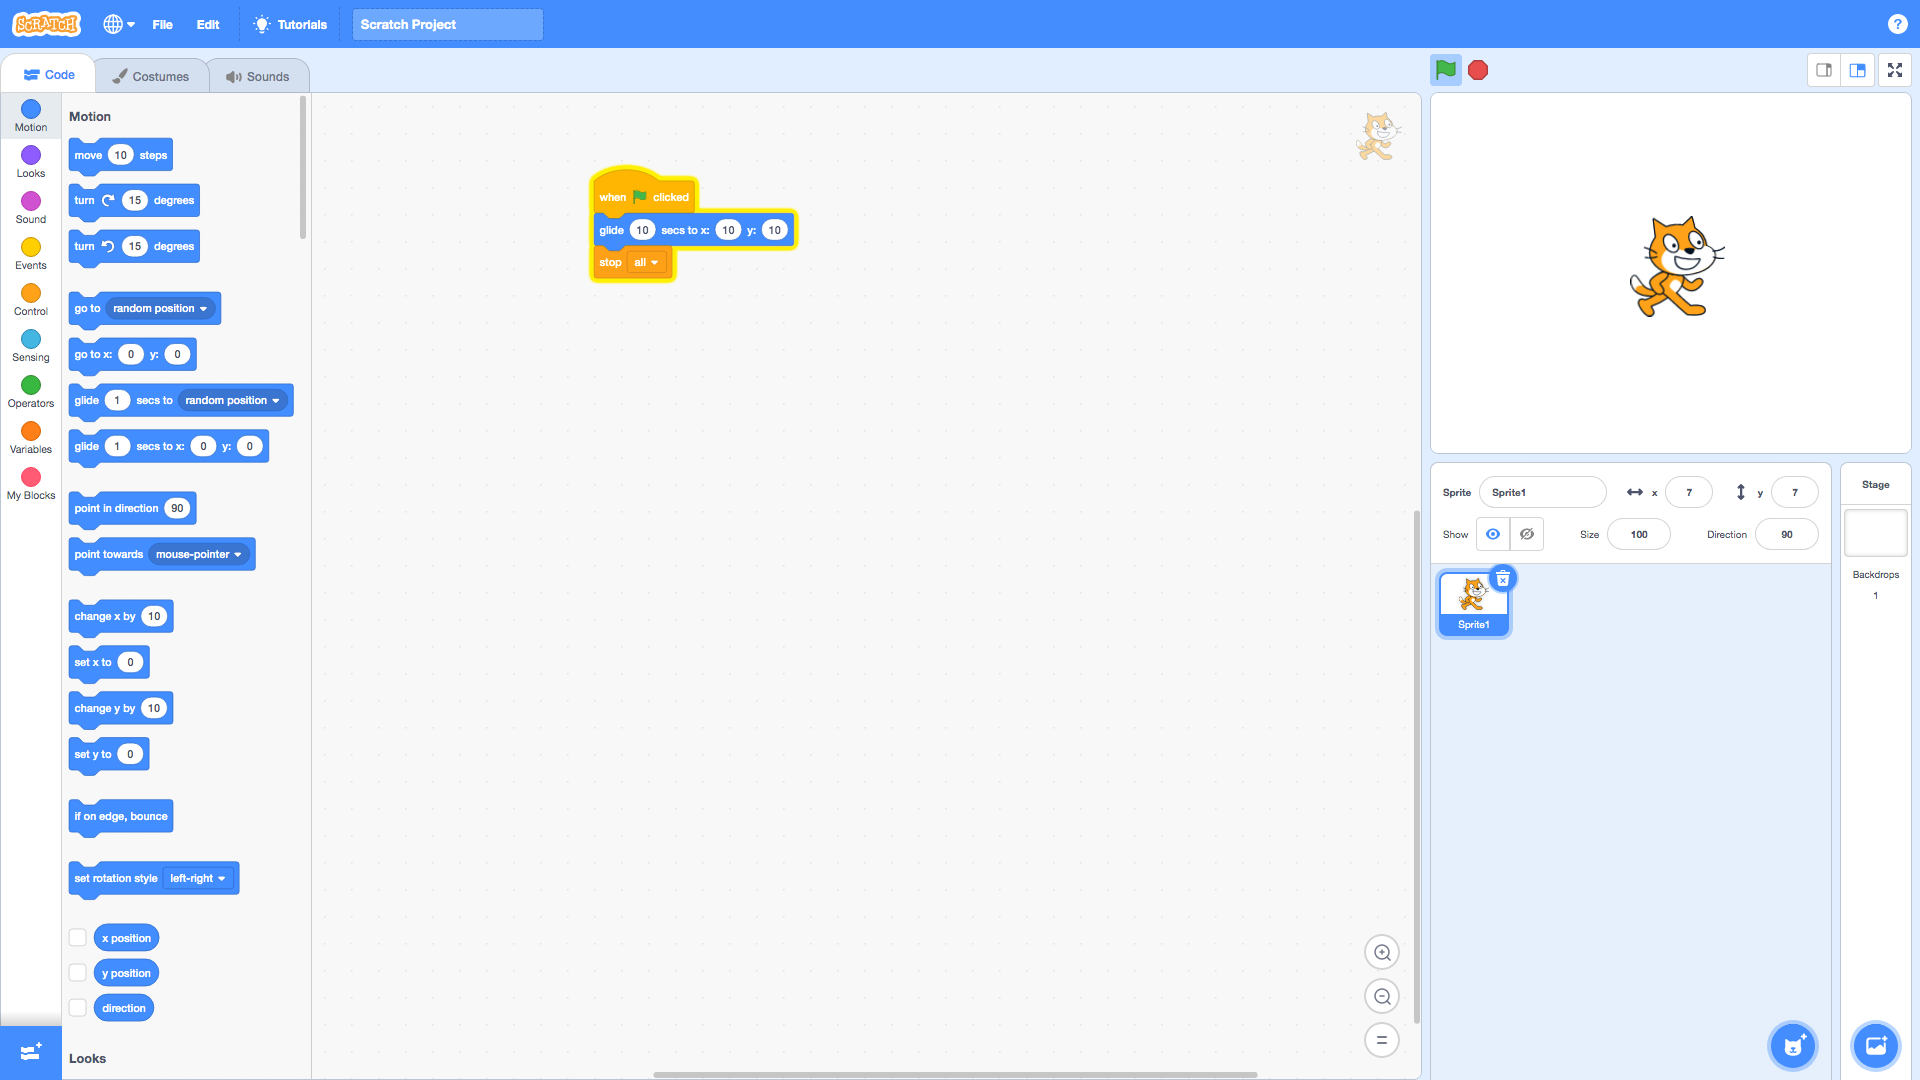
\includegraphics[width=1.0\linewidth,height=0.5\linewidth]{fig0061.png}
  \caption{Плъзгане до зададени координати}
\label{fig0061}
\end{figure}

Анимираният герой има характеристика за ориентация, под формата на ъгъл. При 90 градуса, оранжевата котка гледа на дясно. За да се промени ориентацията на героя се използва блокче с възможност за въвеждане на конкретен ъгъл (Фиг. \ref{fig0062}).

\begin{figure}[H]
  \centering
  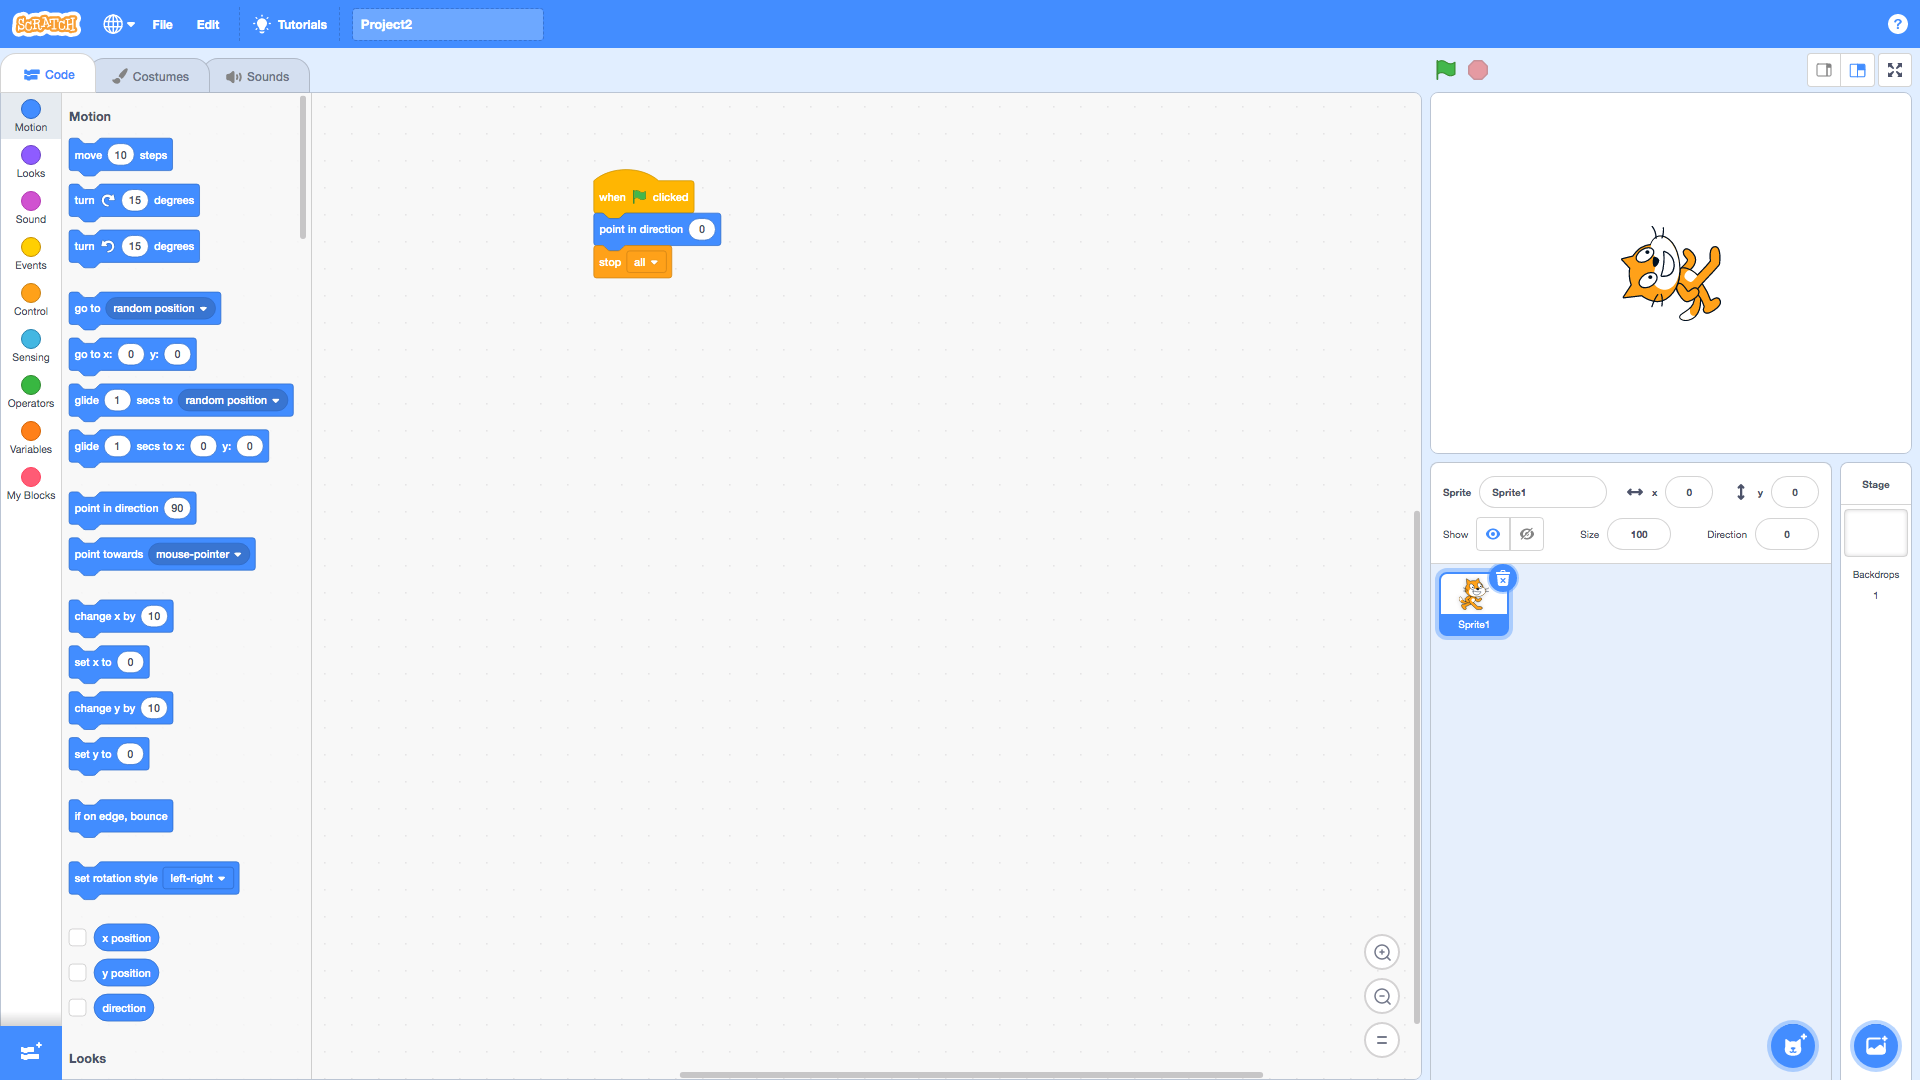
\includegraphics[width=1.0\linewidth,height=0.5\linewidth]{fig0062.png}
  \caption{Ъглова ориентация}
\label{fig0062}
\end{figure}

При по-сложни сценарии за управление на героя, понякога е нужно героят да следи показалеца на мишката. За тази цел има определено блокче, което изпълнява тази инструкция (Фиг. \ref{fig0063}).

\begin{figure}[H]
  \centering
  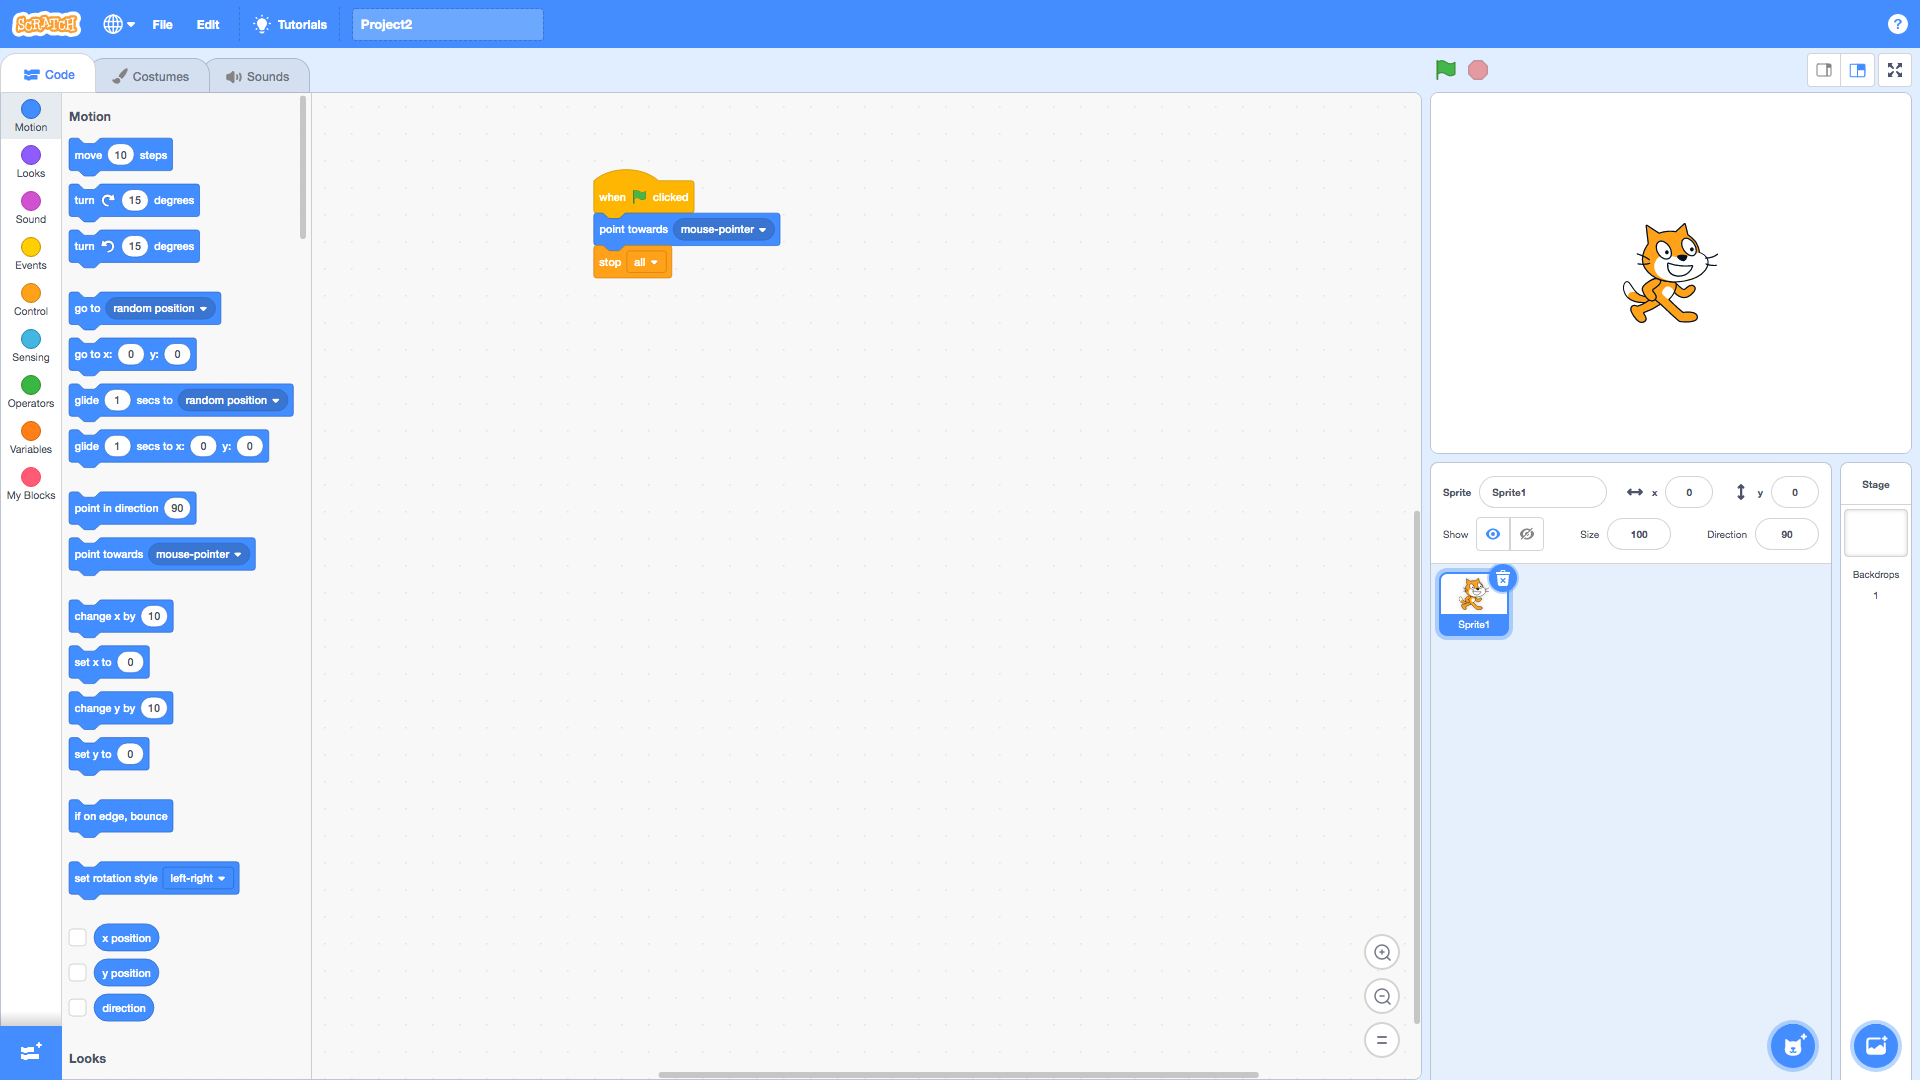
\includegraphics[width=1.0\linewidth,height=0.5\linewidth]{fig0063.png}
  \caption{Ориентация по показалеца на мишката}
\label{fig0063}
\end{figure}

Блокчетата могат да се поставят едно след друго, като за последователна промяна на относителните x и y координатите (относителни, спрямо текущата позиция) на героя има специално определени блокчета (Фиг. \ref{fig0064}).

\begin{figure}[H]
  \centering
  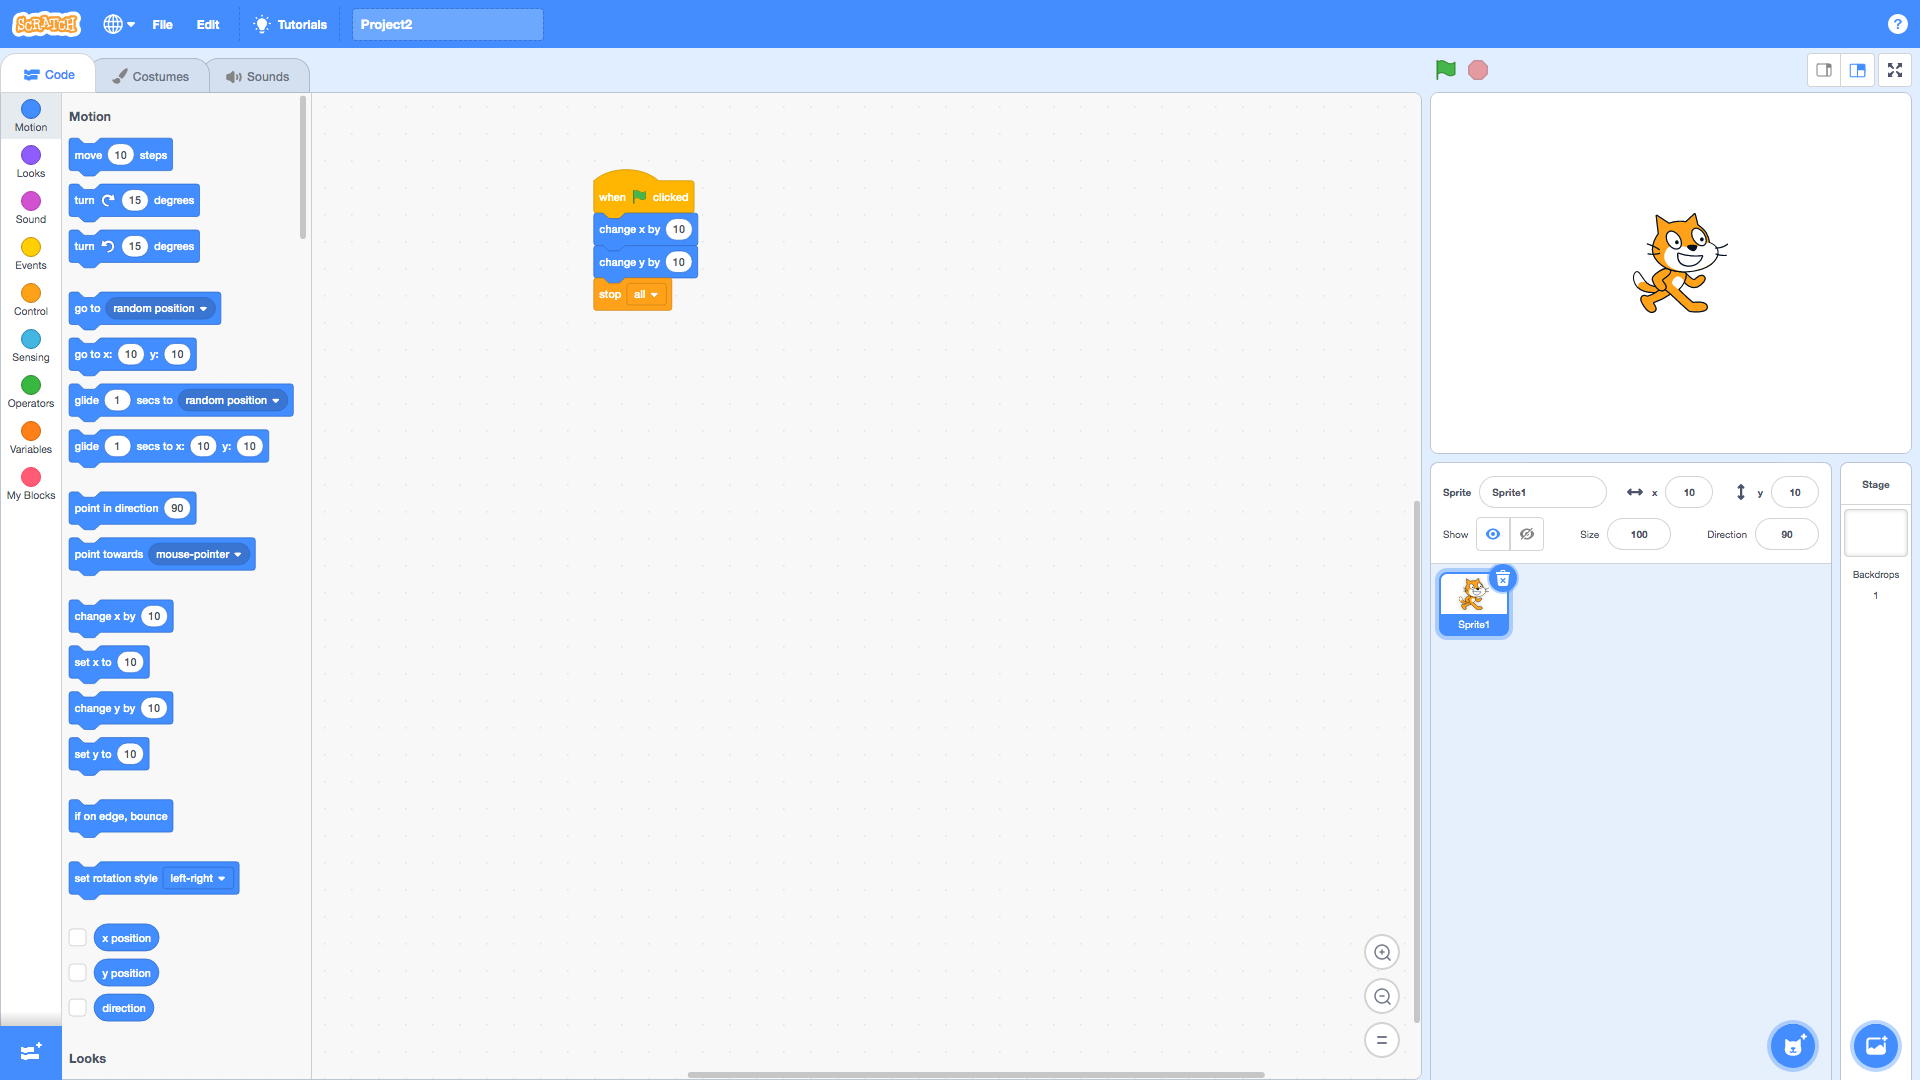
\includegraphics[width=1.0\linewidth,height=0.5\linewidth]{fig0064.png}
  \caption{Последователна промяна на относителни координати}
\label{fig0064}
\end{figure}

Освен относителна промяна на координатите е възможна и абсолютна промяна на координатите, като абсолютната промяна е спрямо центъра на координатната система (Фиг. \ref{fig0065}).

\begin{figure}[H]
  \centering
  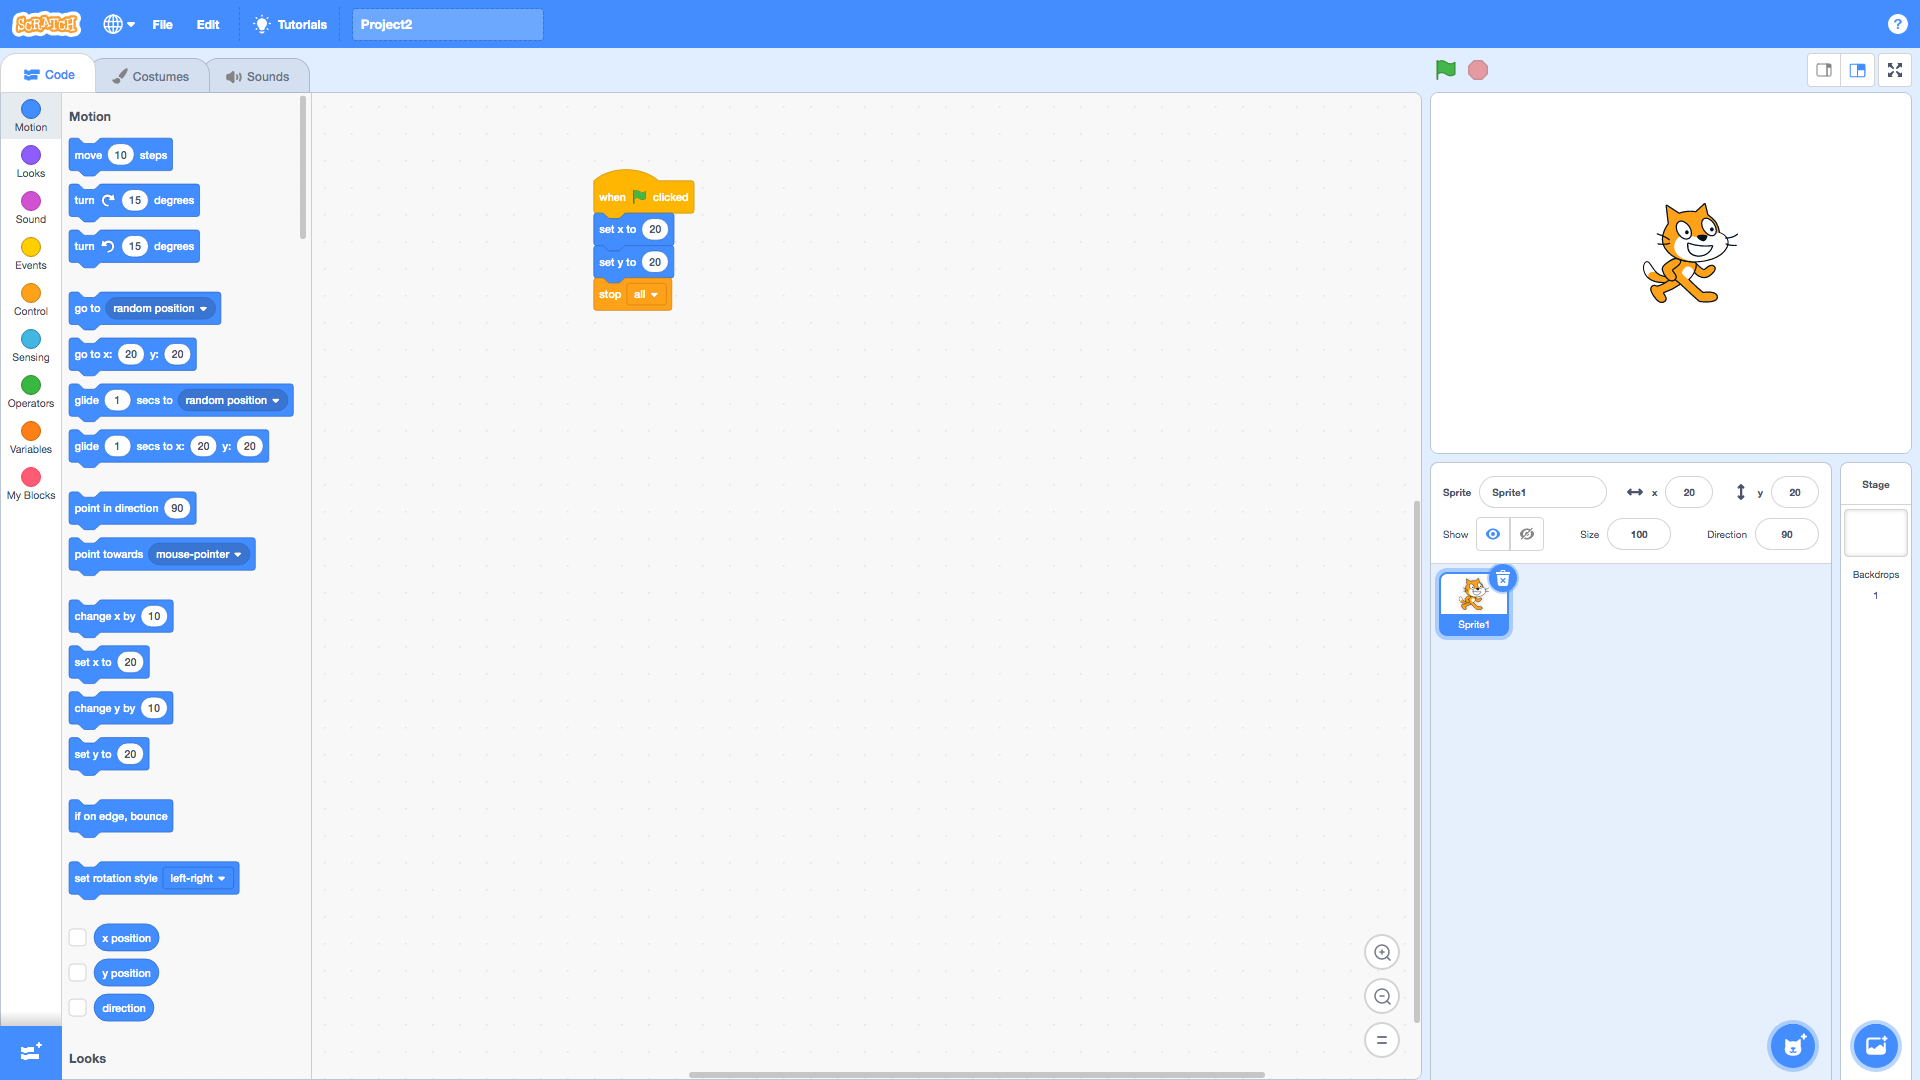
\includegraphics[width=1.0\linewidth,height=0.5\linewidth]{fig0065.png}
  \caption{Последователна промяна на абсолютни координати}
\label{fig0065}
\end{figure}

При своето движение, когато анимираният герой достигне границите на работното пространство, единият вариант е движението да продължи извън видимата зона. Другият вариант е да се вземат мерки и героят да отскача от ръбовете на работното пространство. За това отскачане има конкретно блокче (Фиг. \ref{fig0066}). За да се илюстрира работата му е нужна малко по-сложна последователност от инструкции. При всяко стартиране на програмата, първо се променят относителните координати, а след това се извършва отскачане от ръба, ако е необходимо. За да бъде малко по-интересен сценарият за проверка, вместо фиксирани стойности за относително отместване се използва вграждане на едно от зелените блокчета, което позволява генериране на случайно число в предварително определен диапазон. Съществено е да се забележи, че зеленото блокче има овална форма, което подсказва, че то е предназначено за вграждане в някой от другите блокове, които имат овален слот. 

\begin{figure}[H]
  \centering
  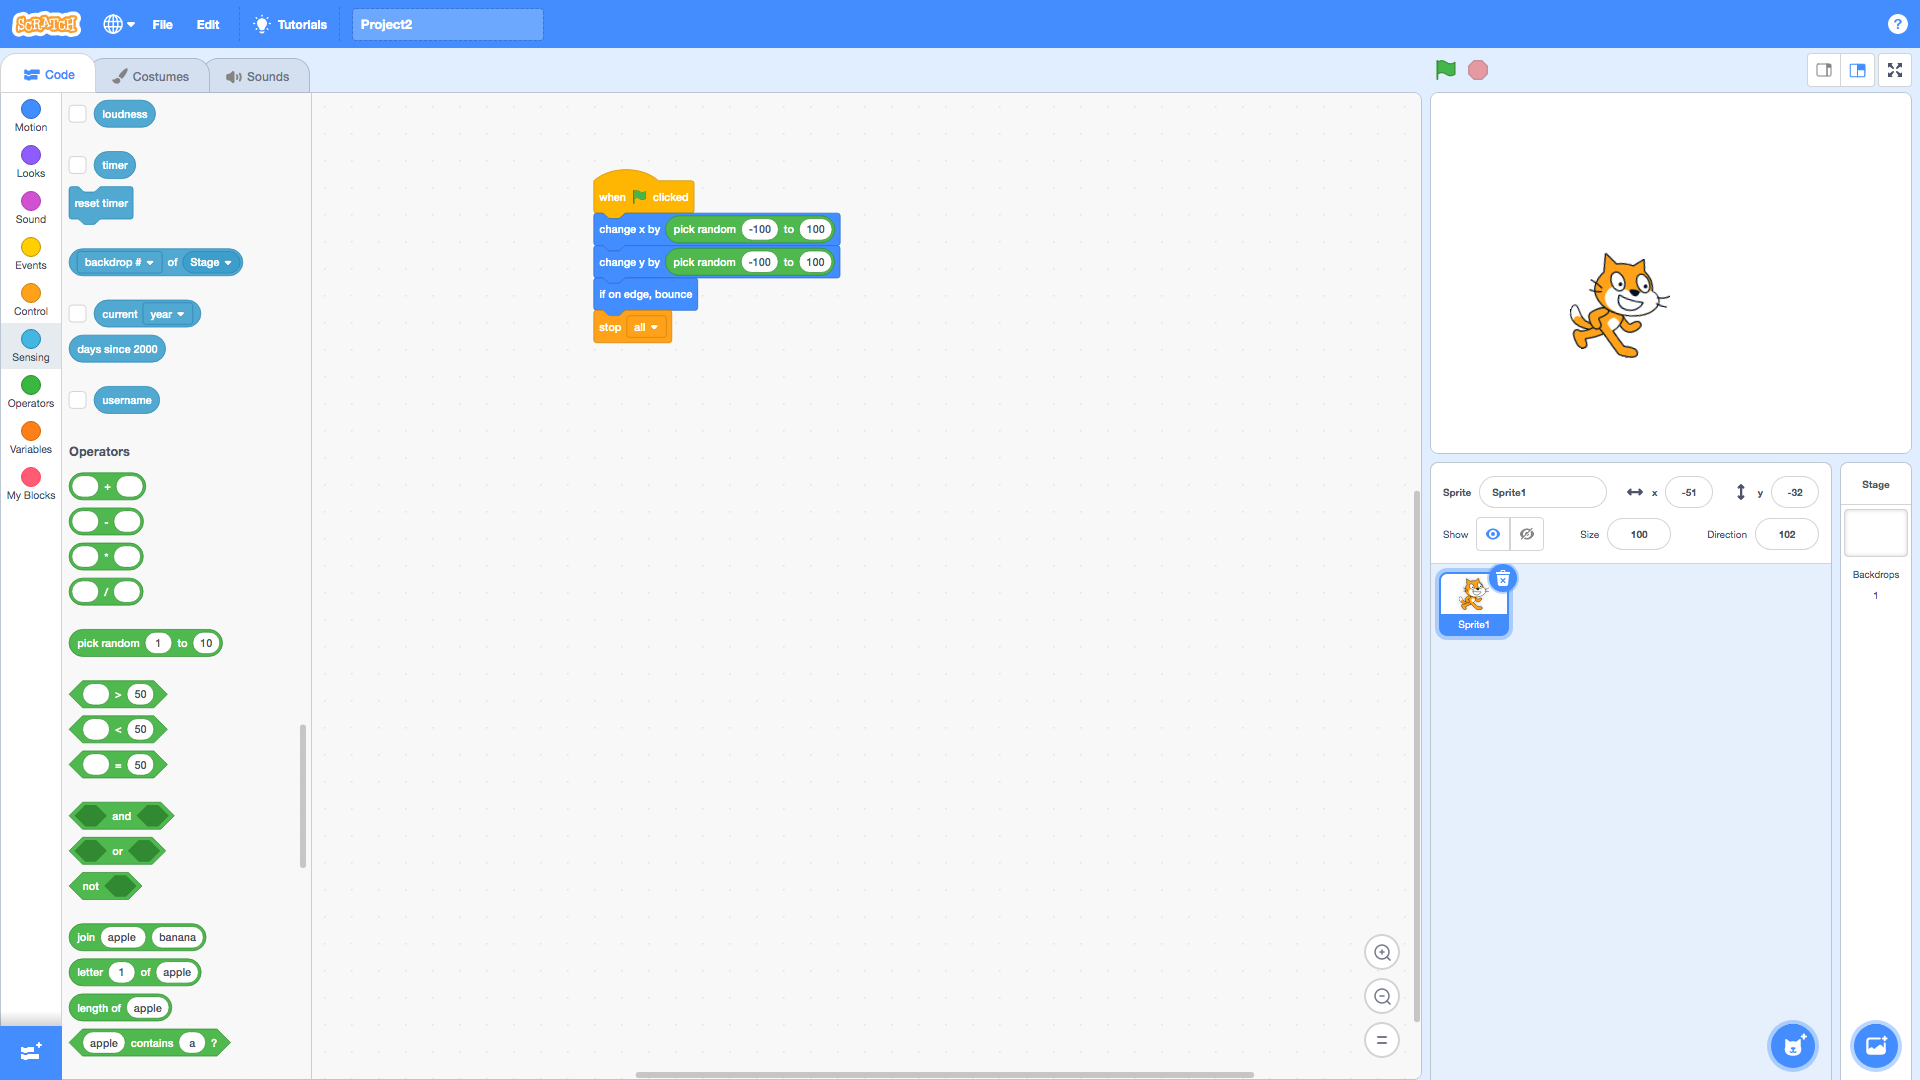
\includegraphics[width=1.0\linewidth,height=0.5\linewidth]{fig0066.png}
  \caption{Отскачане от ръбовете}
\label{fig0066}
\end{figure}

Следващо, много полезно блокче, от групата на тъмно оранжевите е блокчето за изчакване на период от време (Фиг. \ref{fig0067}). Когато това блокче бъде поставено между блокчетата за начало и край, програмата изчаква зададения брой секунди, преди да преустанови изпълнението си. По време на изпълнение, ясно може да се забележи, че около последователността от инструкции се появява жълта рамка, която символизира режима на изпълняващи се инструкции. 

\begin{figure}[H]
  \centering
  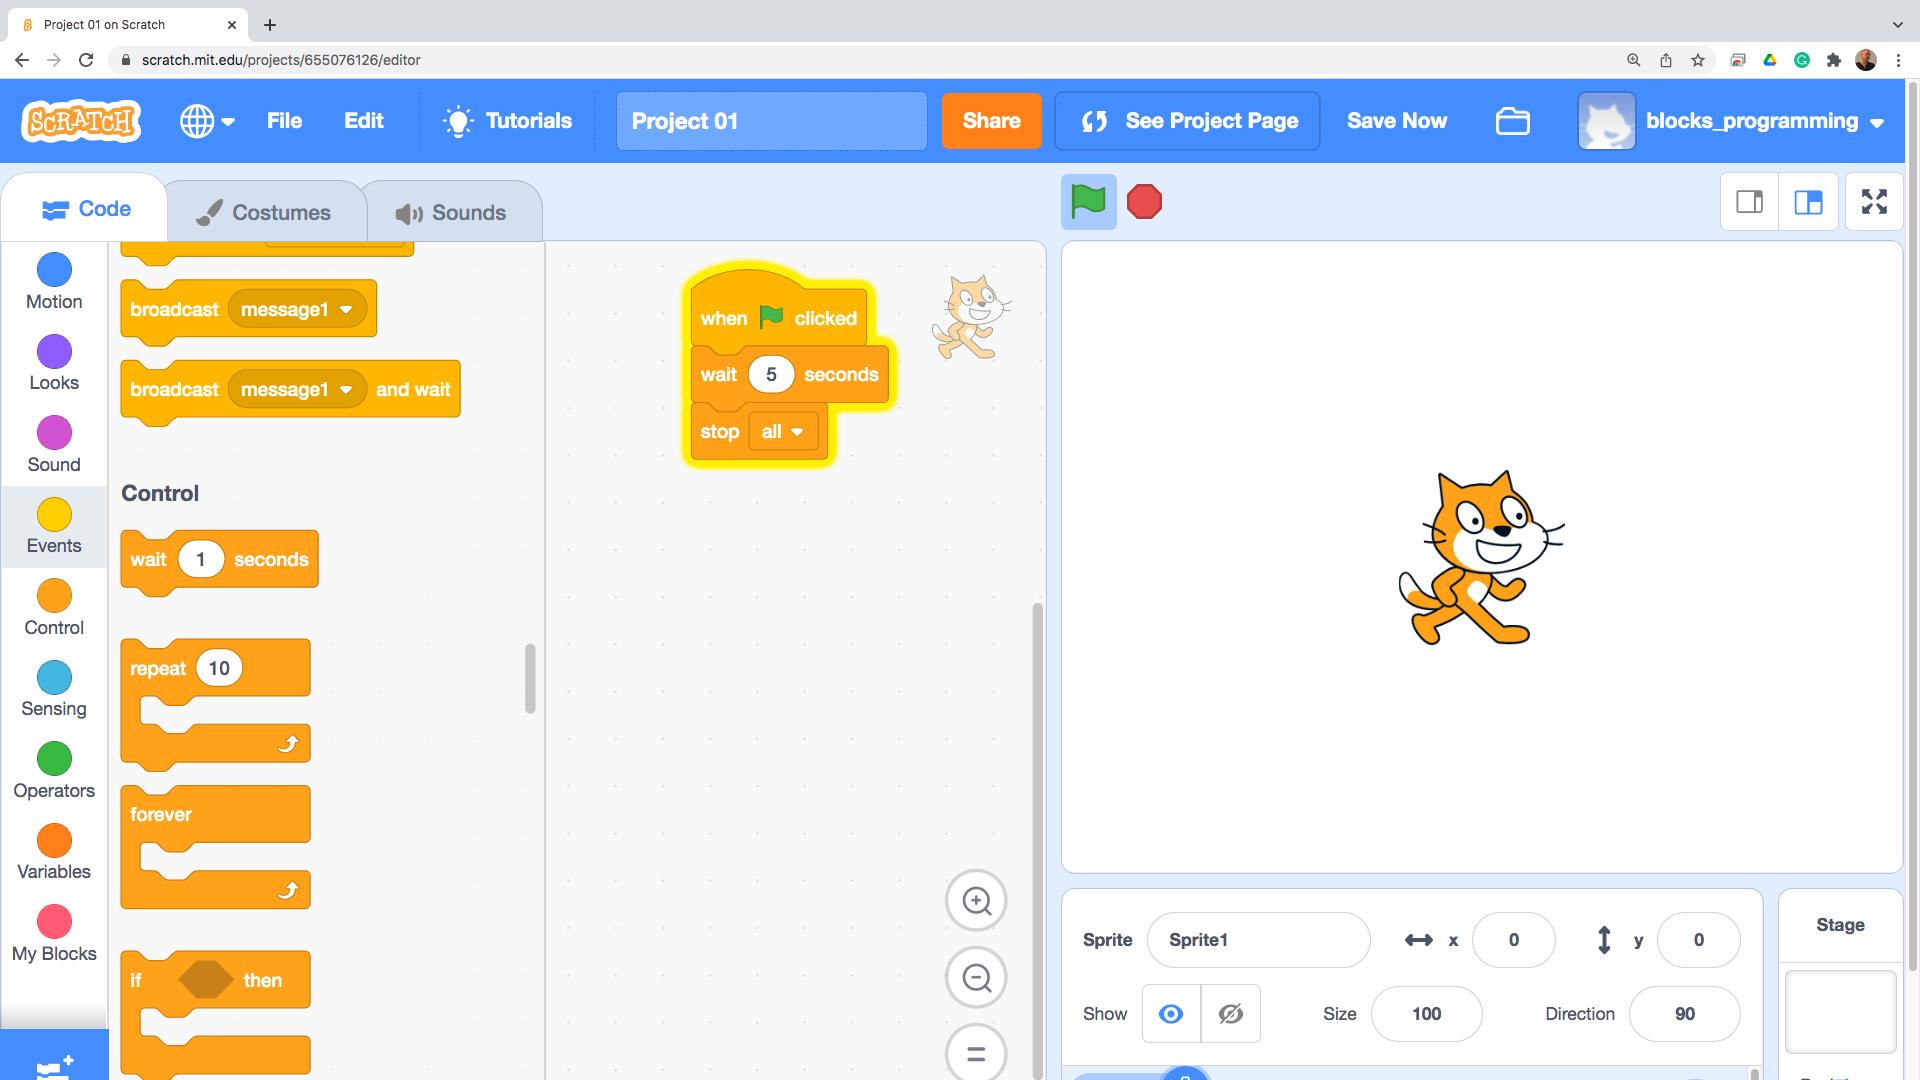
\includegraphics[width=1.0\linewidth,height=0.5\linewidth]{fig0067.png}
  \caption{Инструкция за изчакване}
\label{fig0067}
\end{figure}

Групата на лилавите блокчета съдържат инструкции за външното оформление на анимирания герой. Първите две блокчета са предназначени за реплики (Фиг. \ref{fig0068}), които героят казва (изписват се както в комикс). Първото блокче задава текст, който стои на екрана до следващата инструкция. Точно за това е нужно да има няколко секунди изчакване, така че текстът да остане видим за потребителя. Второто блокче има и параметър с който да се определи колко секунди текстът да бъде видим за потребителя. 

\begin{figure}[H]
  \centering
  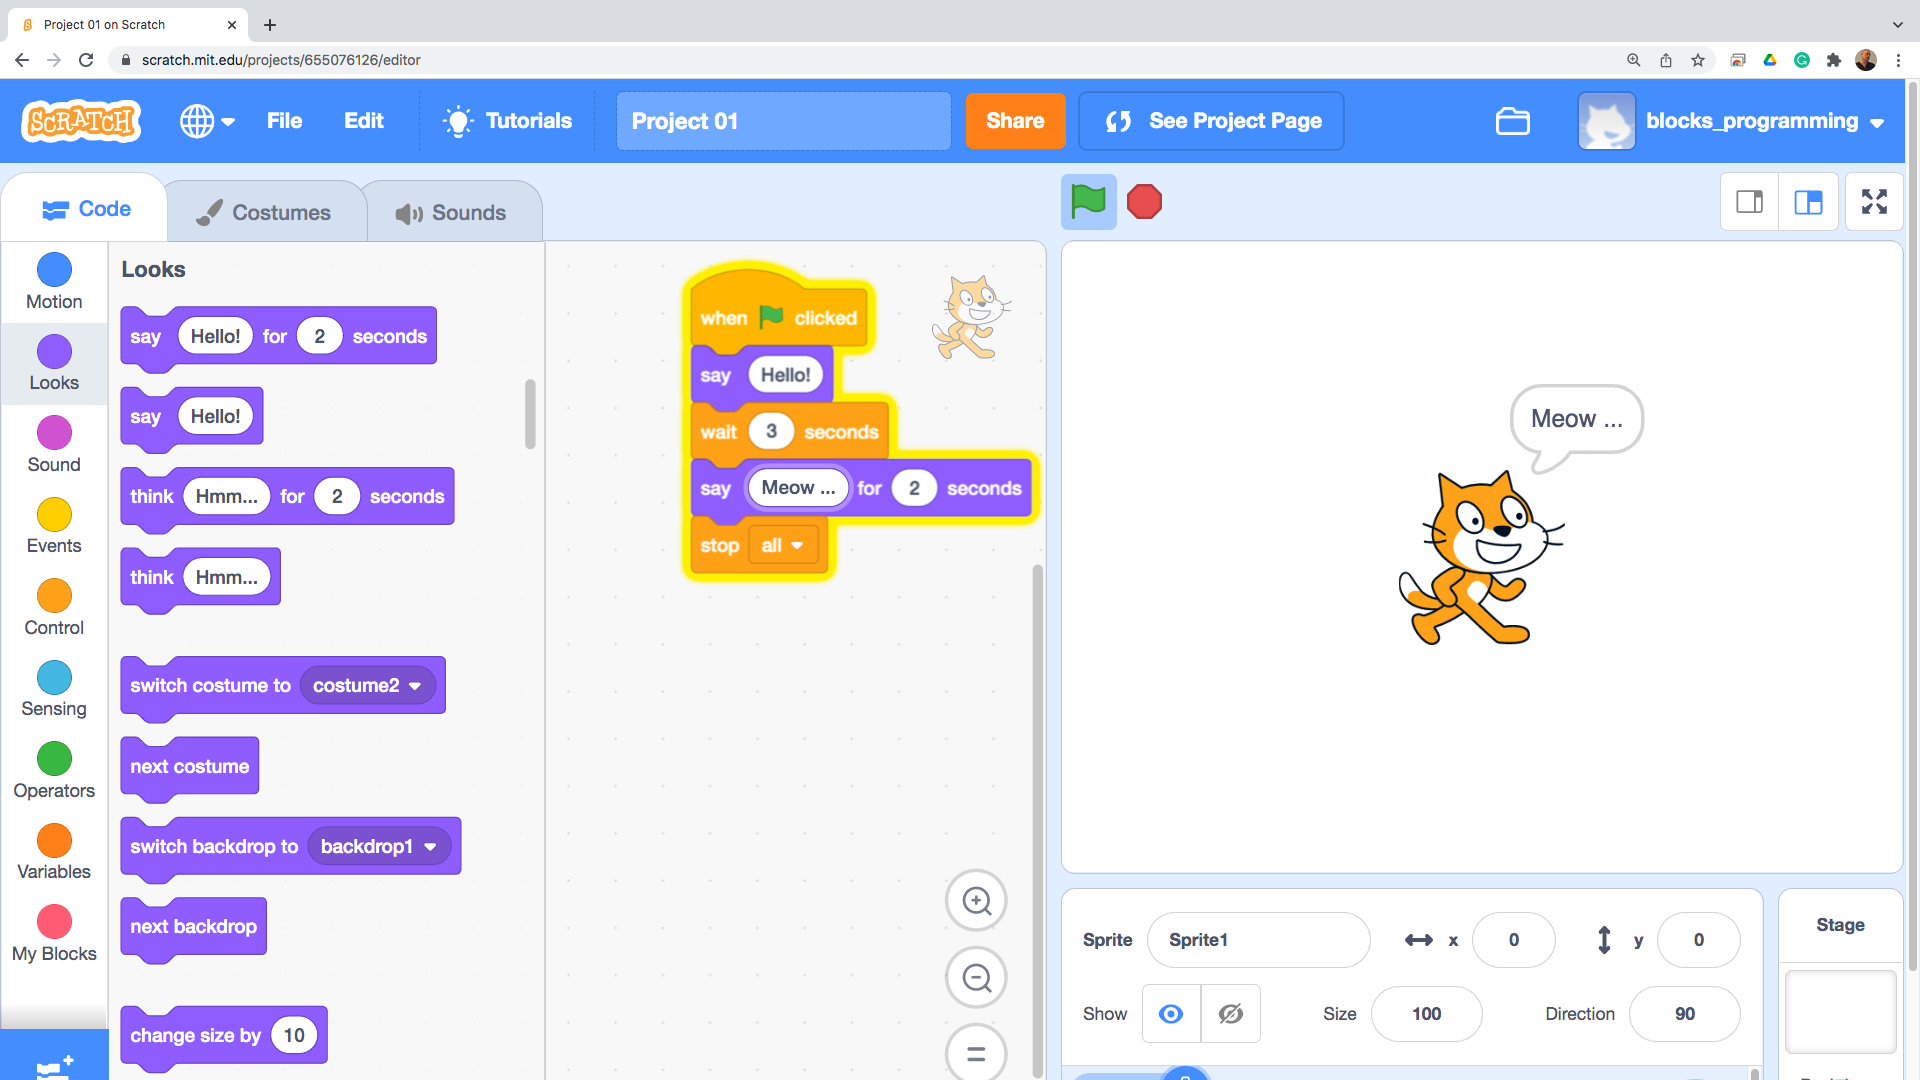
\includegraphics[width=1.0\linewidth,height=0.5\linewidth]{fig0068.png}
  \caption{Изписване на реплики за изговаряне}
\label{fig0068}
\end{figure}

Вторите две блокчета са предвидени за реплики, които анимираният герой си мисли, но не изрича. Разликата се състои в начина по който се визуализира текстът (Фиг. \ref{fig0069}).

\begin{figure}[H]
  \centering
  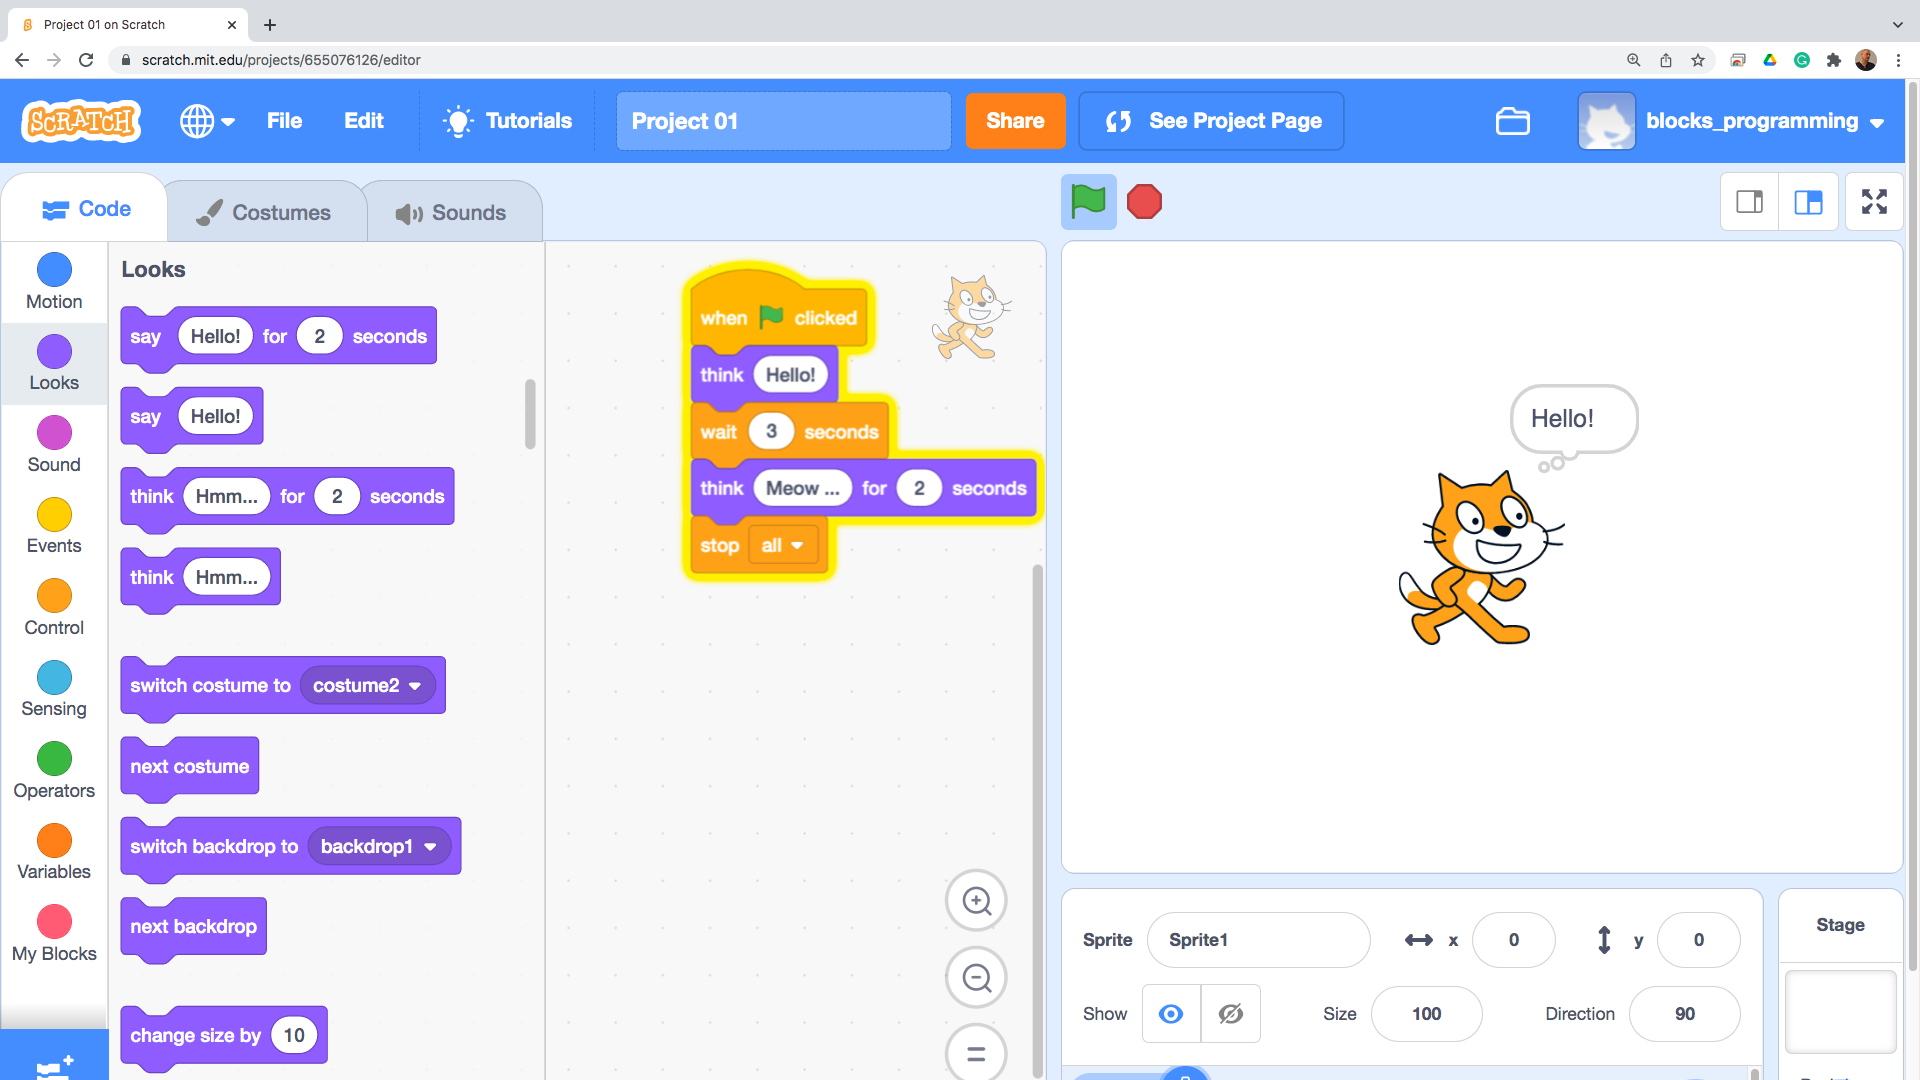
\includegraphics[width=1.0\linewidth,height=0.5\linewidth]{fig0069.png}
  \caption{Изписване на реплики, като мисъл}
\label{fig0069}
\end{figure}

Анимираните герои в Scratch са под формата на спрайтове. Спрайтът е набор от различни изображения за героя в различни пози. За смяната на тези различни пози се използват две блокчета (Фиг. \ref{fig0070}), като първото задава конкретен кадър в спрайта, а второто задава следващия кадър в последователността.

\begin{figure}[H]
  \centering
  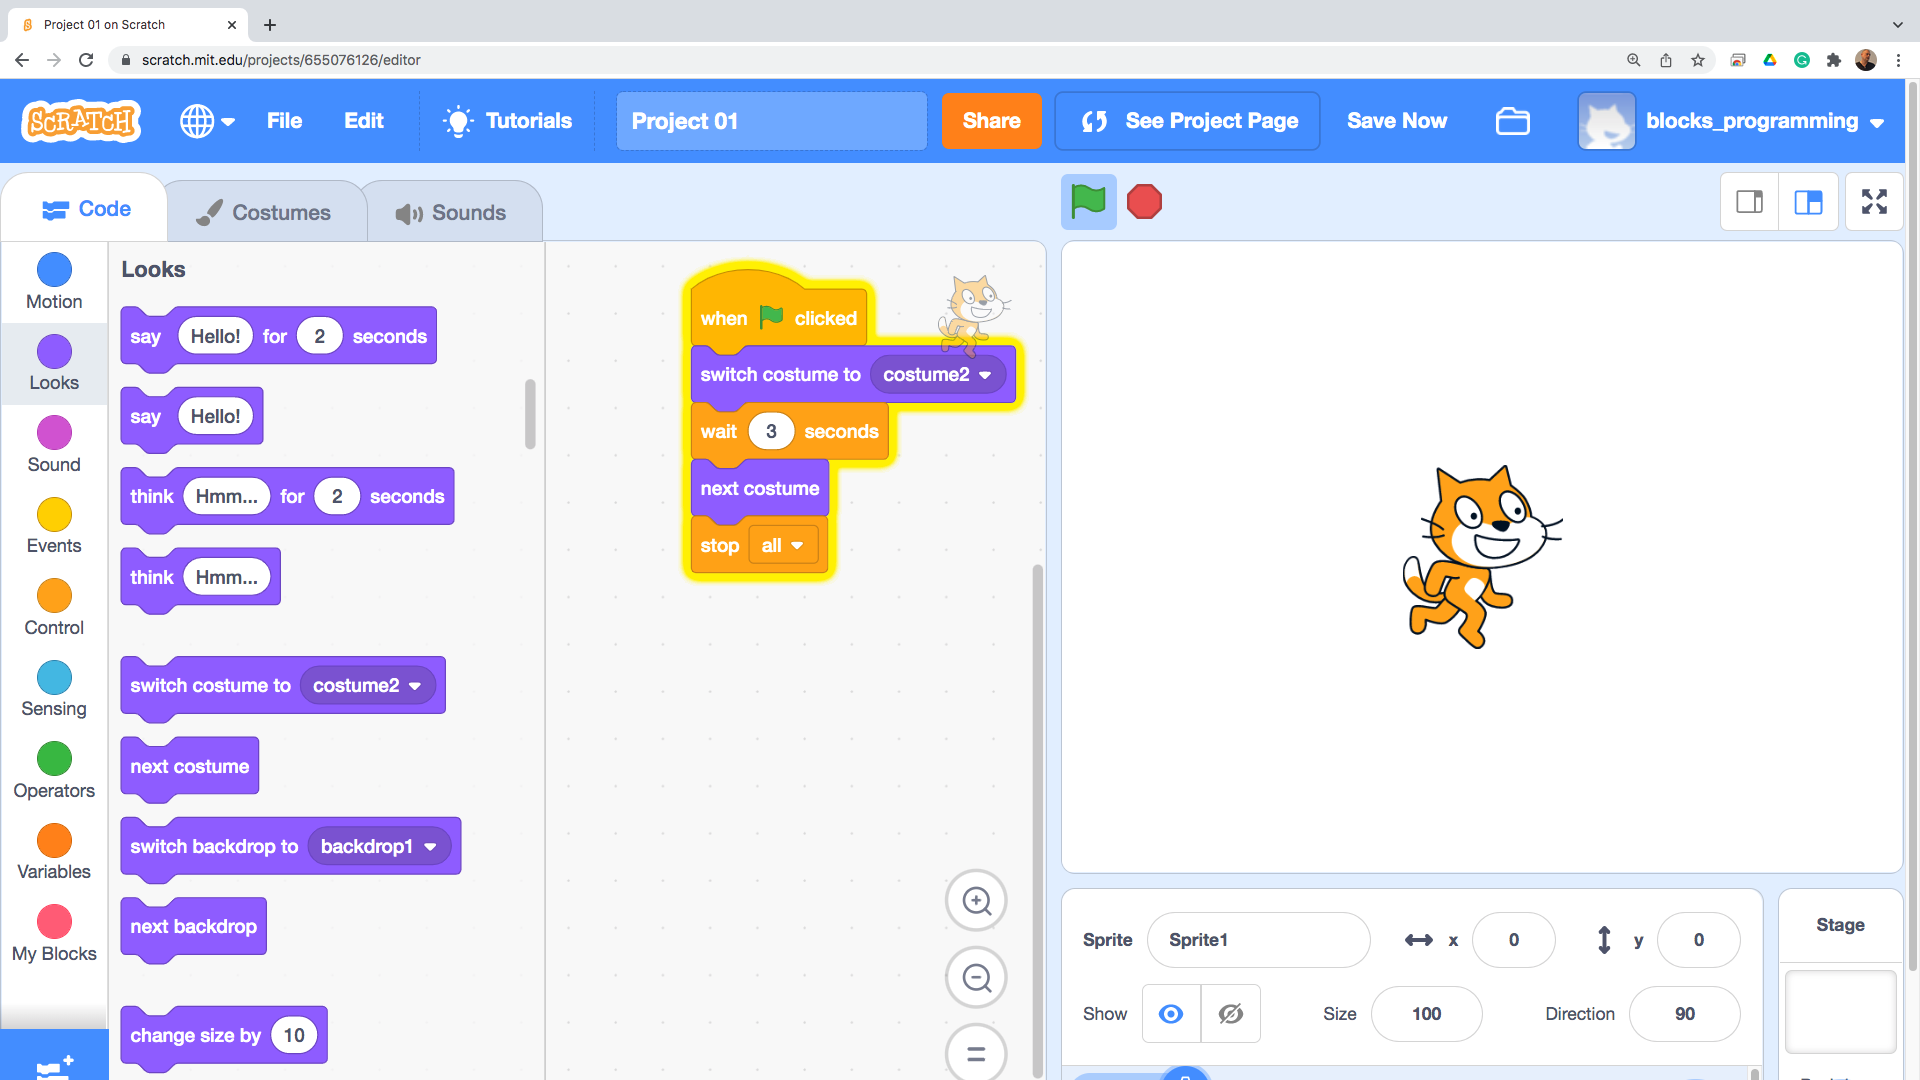
\includegraphics[width=1.0\linewidth,height=0.5\linewidth]{fig0070.png}
  \caption{Смяна на пози}
\label{fig0070}
\end{figure}

На работната сцена освен анимираните герои (под формата на спрайтове) има и фоново изображение. Това фоново изображение също подлежи на промяна, за което са предвидени две отделни блочета (Фиг. \ref{fig0071}). С първото може да се избират фонови изображения напред, назад, по случаен принцип или с конкретно название, а с второто блокче следващото изображение в последователността. 

\begin{figure}[H]
  \centering
  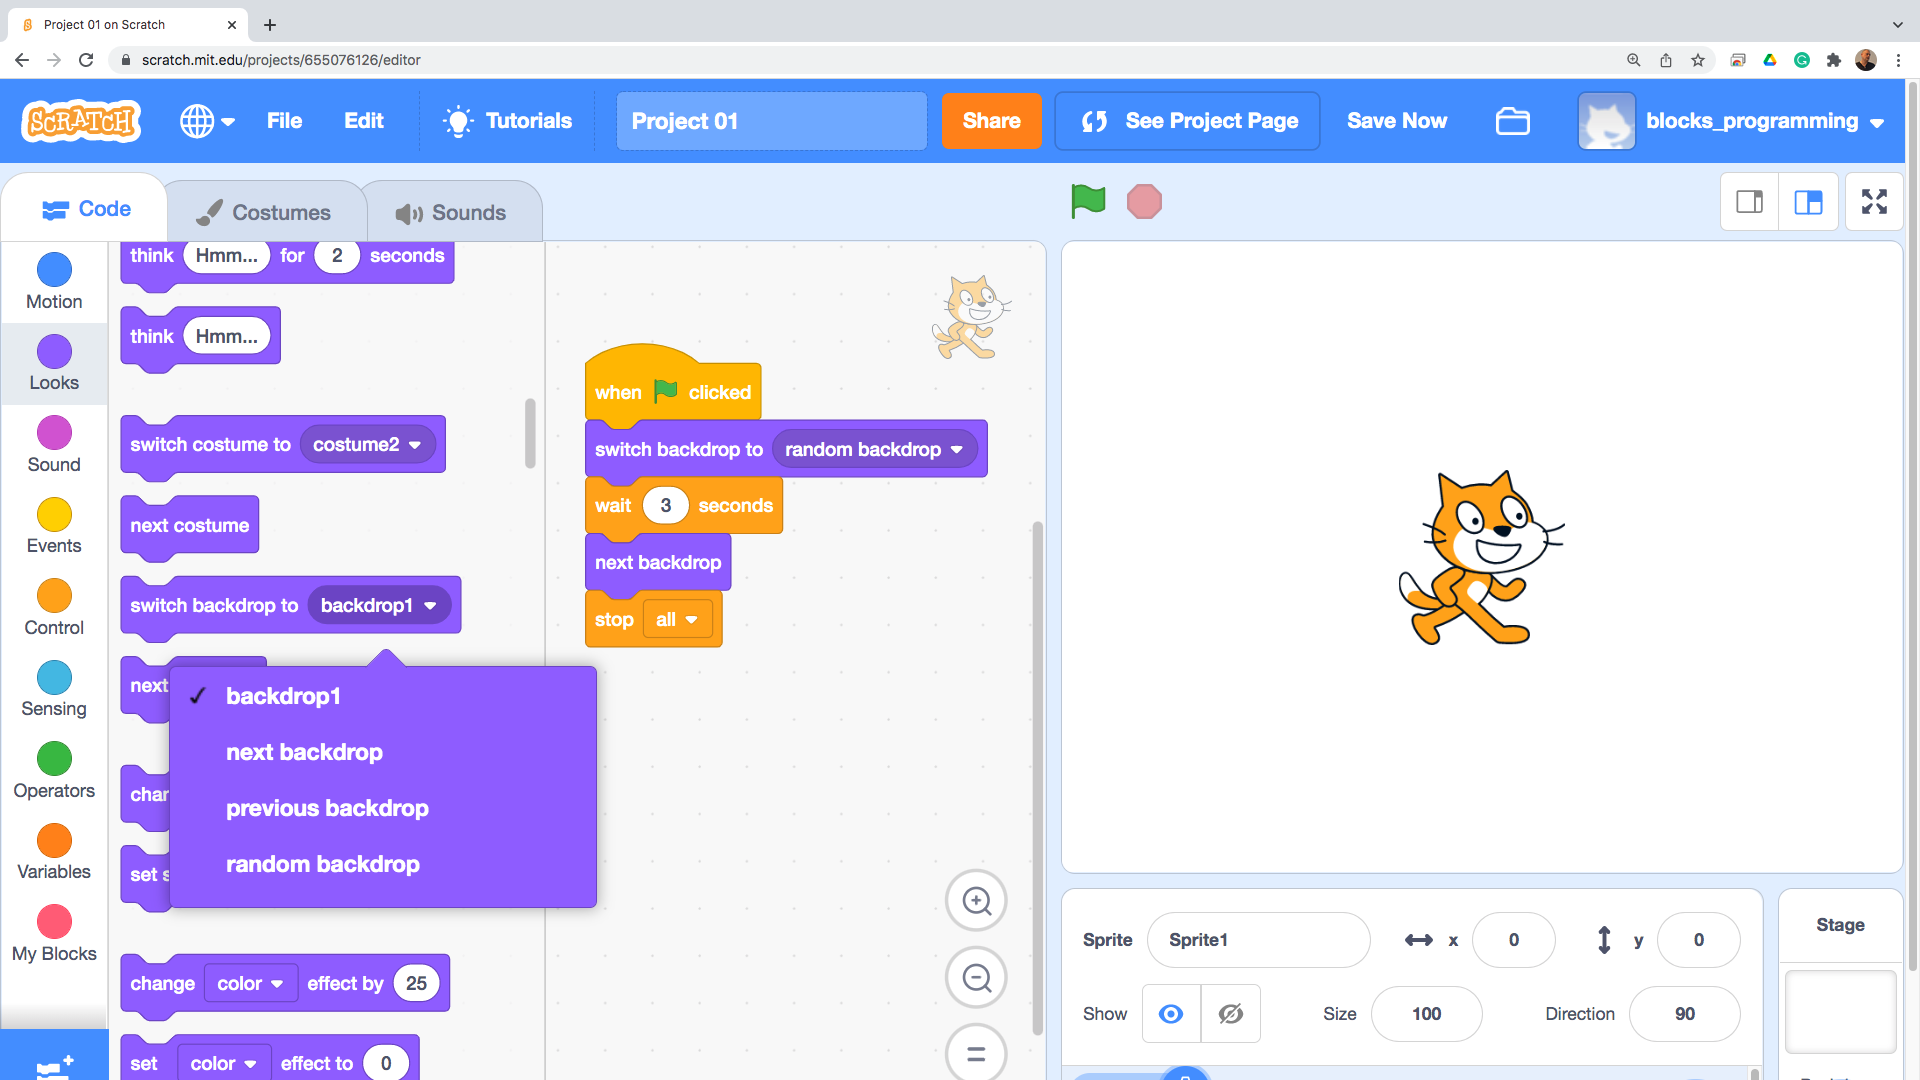
\includegraphics[width=1.0\linewidth,height=0.5\linewidth]{fig0071.png}
  \caption{Смяна на фона}
\label{fig0071}
\end{figure}

За промяната на размера на анимирания герой има две конкретни блокчета, като първото променя размера в абсолютни стойности, а второто променя размера в проценти, спрямо оригиналния размер (Фиг. \ref{fig0072}).

\begin{figure}[H]
  \centering
  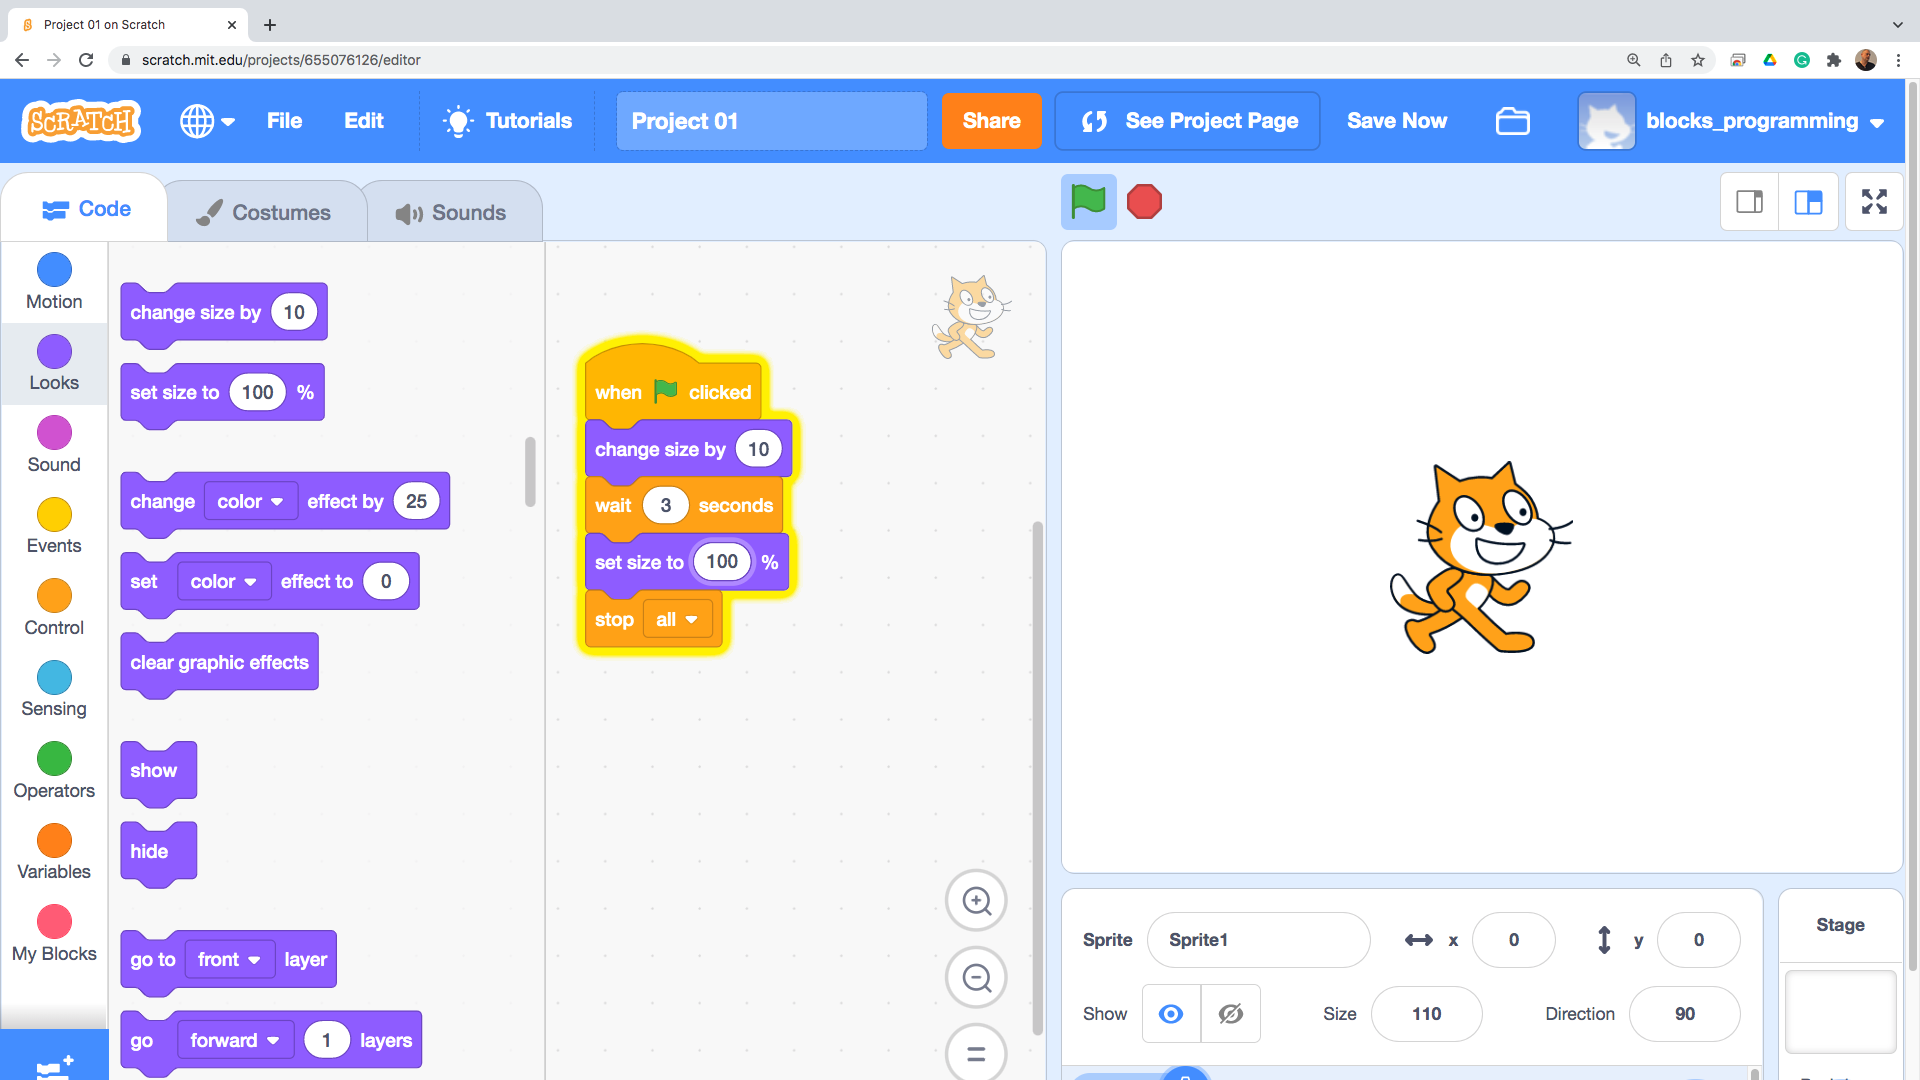
\includegraphics[width=1.0\linewidth,height=0.5\linewidth]{fig0072.png}
  \caption{Промяна на размерите}
\label{fig0072}
\end{figure}

За промяна на визуалното оформление на анимирания герой са предвидени три блокчета (Фиг. \ref{fig0073}). Първите две задават промяна, като промяната може да бъде в цвета, различни изкривявания, пикселизация, мозайка, прозрачност или яркост, а третото блокче отменя всички направени декорации. Първото блокче предизвиква относителна промяна, спрямо текущото състояние на героя, а второто блокче задава абсолютна промяна. Отново е важно да се дадат няколко секунди, така че промените да бъдат ясно различими. 

\begin{figure}[H]
  \centering
  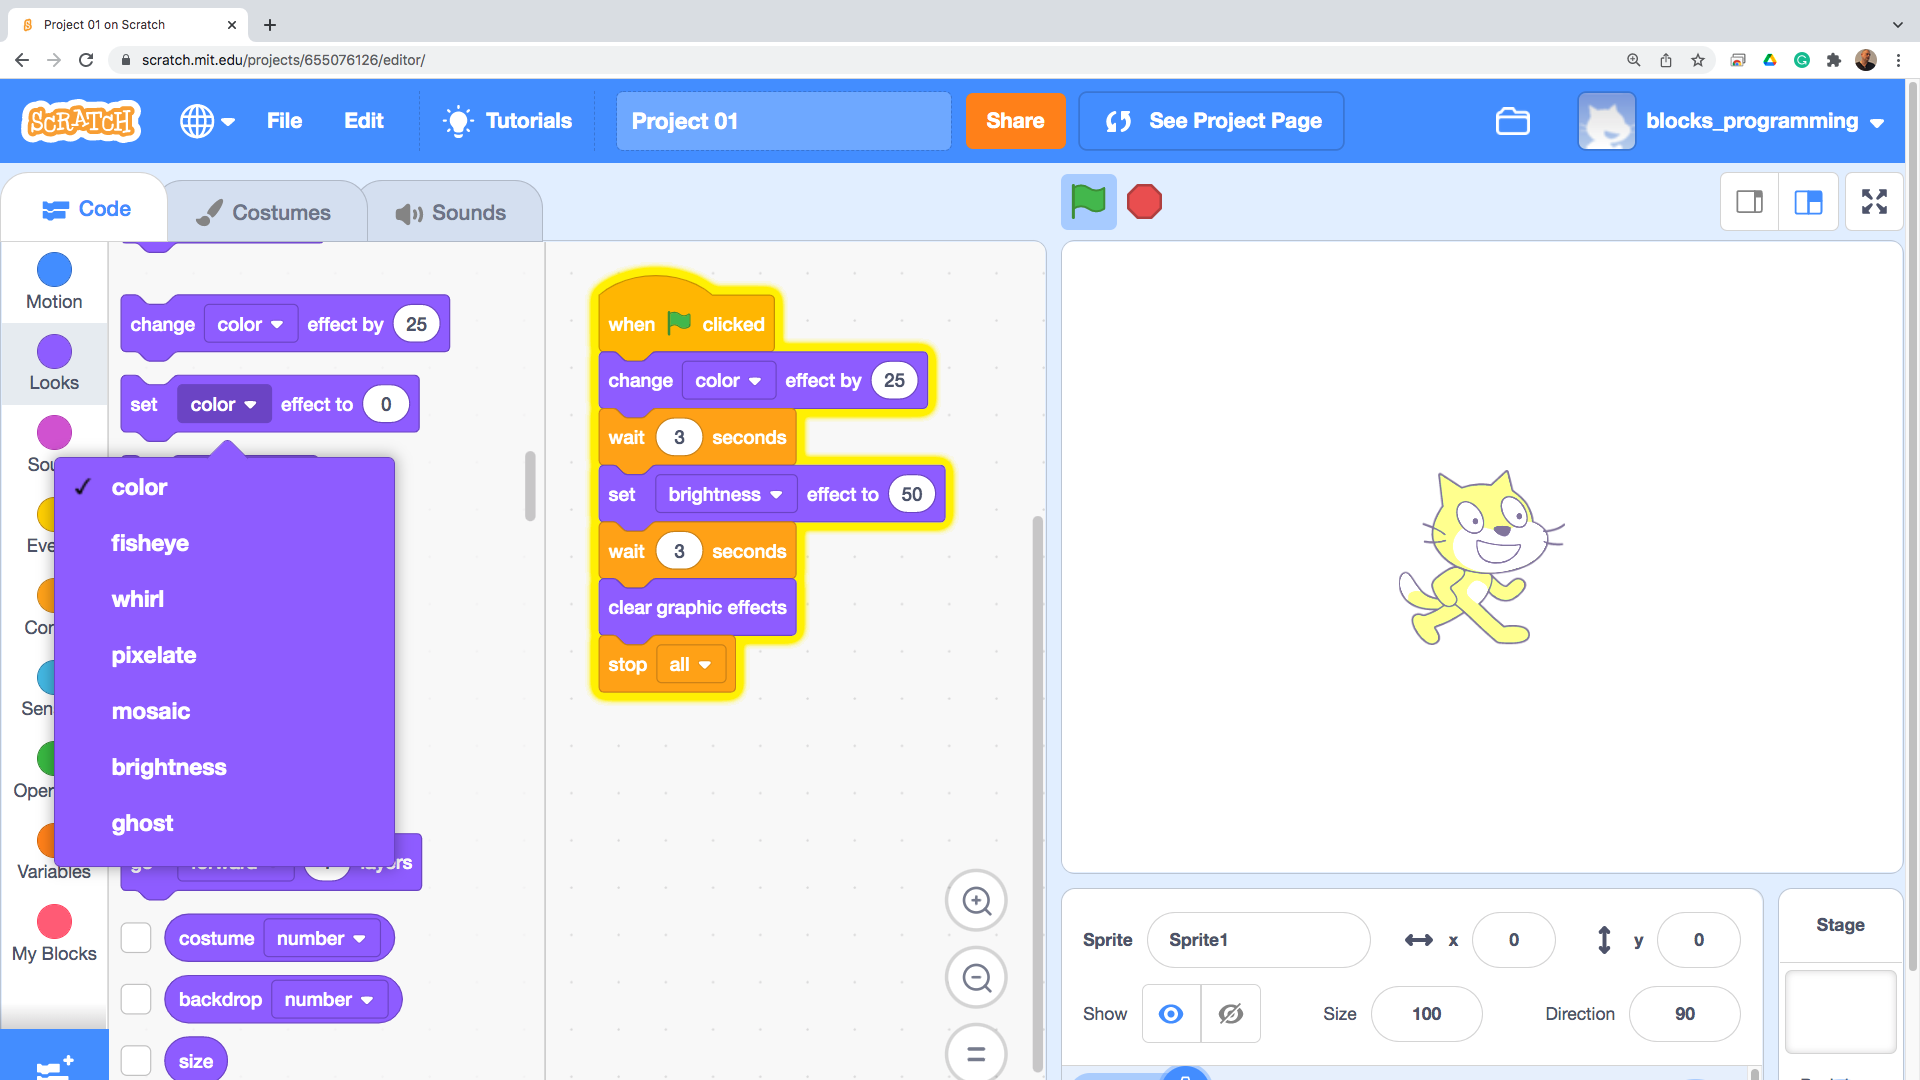
\includegraphics[width=1.0\linewidth,height=0.5\linewidth]{fig0073.png}
  \caption{Промяна на външния вид}
\label{fig0073}
\end{figure}

Работата със спрайтове е предимно за постигане на анимирани ефекти. Различните анимирани герой в сцената имат определени взаимодействия по между си. Сценарият на изработвания проект определя в кой момент всеки от героите се появява на сцената и в кой момент изчезва. За да се осъществи появата и изчезването са предвидени две блокчета, извършващи тези действия (Фиг. \ref{fig0074}).

\begin{figure}[H]
  \centering
  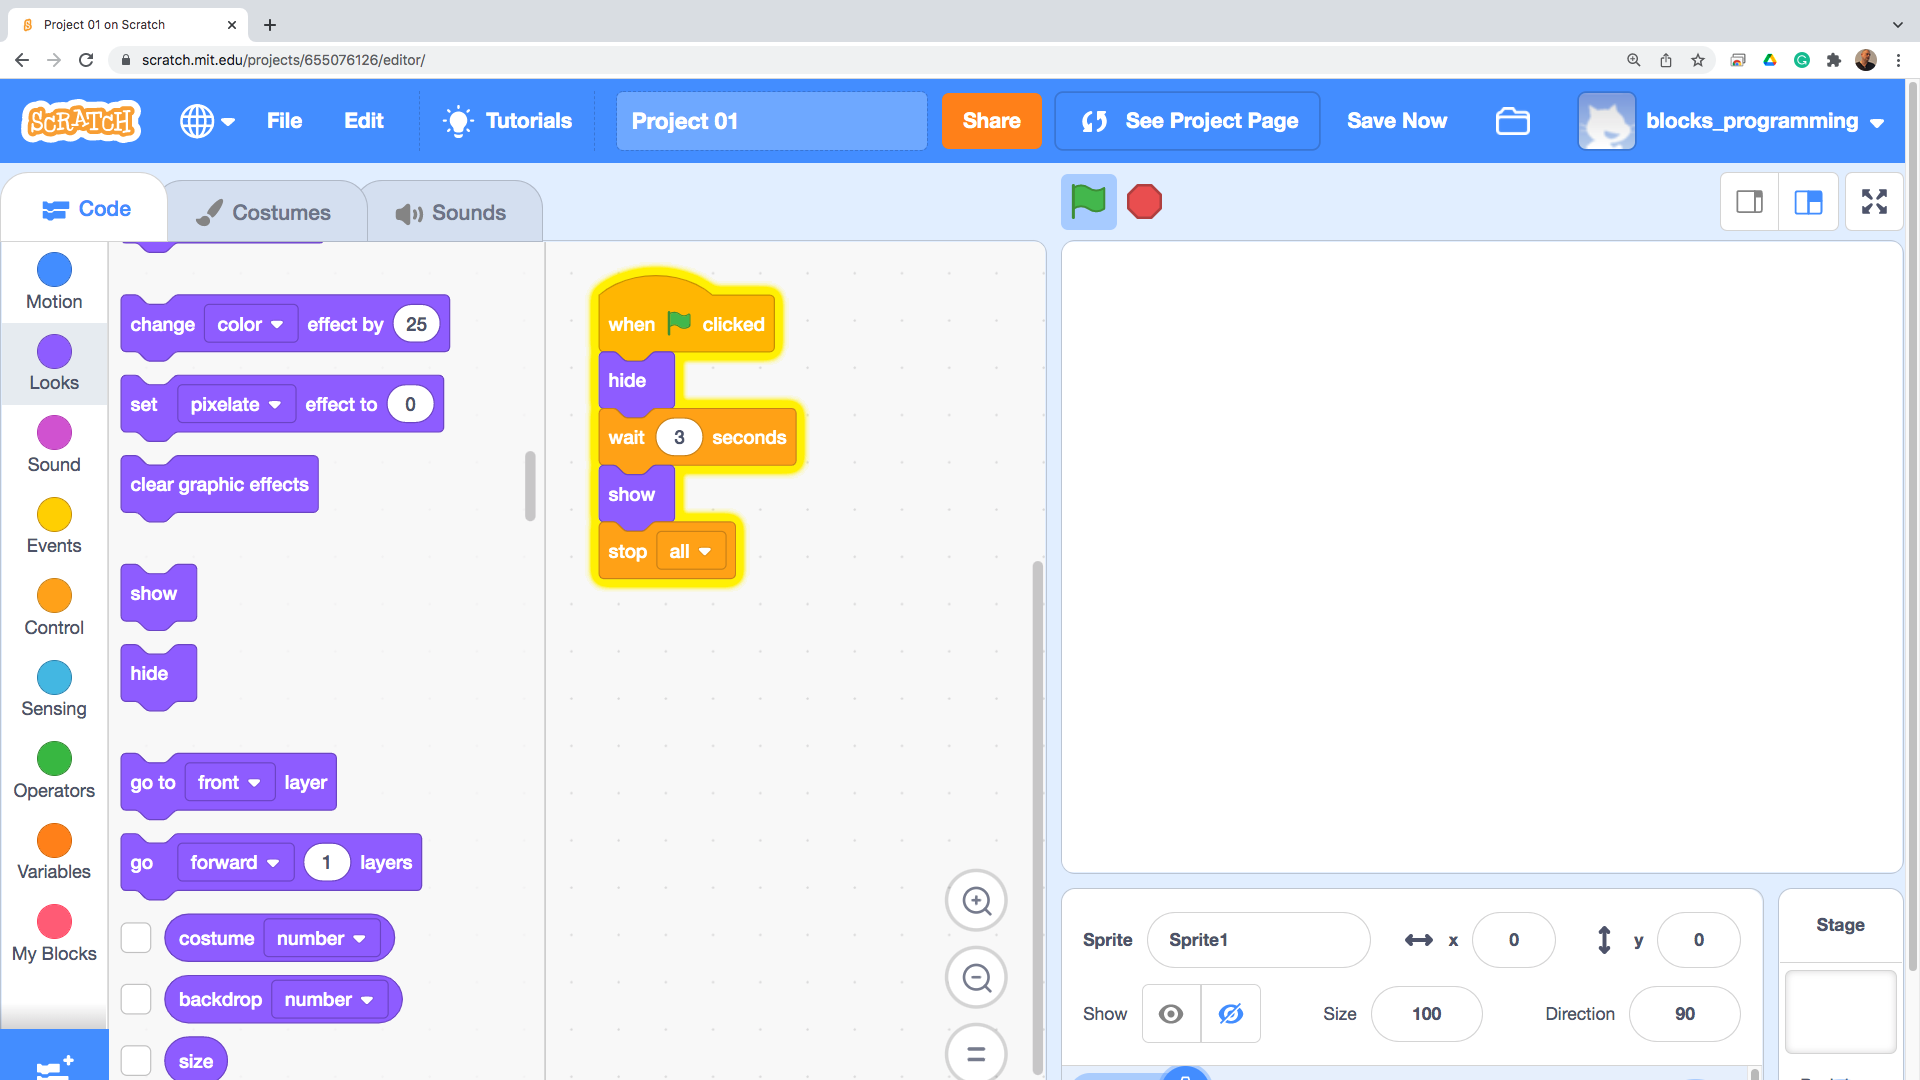
\includegraphics[width=1.0\linewidth,height=0.5\linewidth]{fig0074.png}
  \caption{Скриване и повява}
\label{fig0074}
\end{figure}

Множество програмни продукти, работещи с растерни графични изображения, организират различните изображения в слоеве. Пример за такива са Adobe Photoshop, GIMP, Microsoft Word, LibreOffice Draw и много други. Организацията в слоеве е логична, тъй като различните спрайтове в определени моменти от времето могат да се припокриват. В някои от софтуерните пакети за графична обработка, наличието на слоеве се възприема като Z буфер. В Scratch също е налична възможността за работа със слоеве, като две конкретни блокчета позволяват спрайтът да се придвижва напред и назад по слоевете (Фиг. \ref{fig0075}).

\begin{figure}[H]
  \centering
  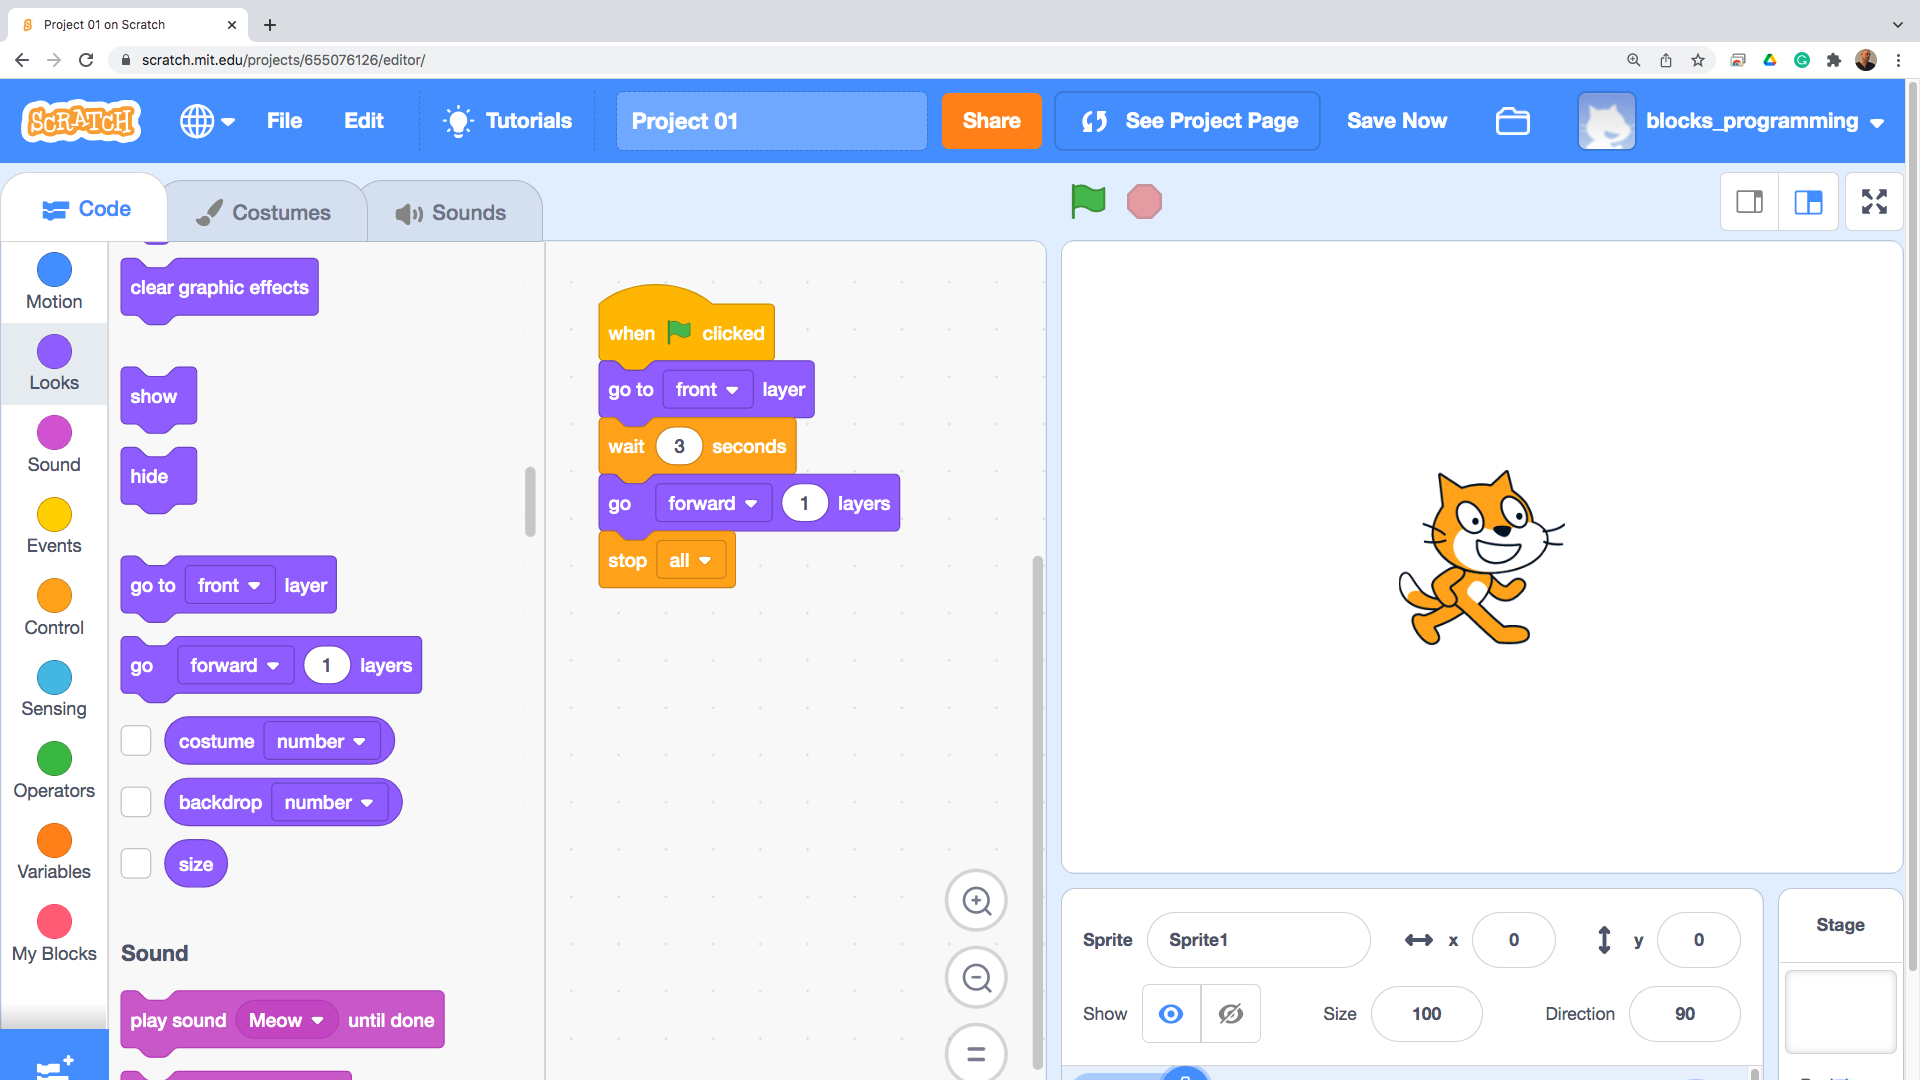
\includegraphics[width=1.0\linewidth,height=0.5\linewidth]{fig0075.png}
  \caption{Придвижване по слоевете}
\label{fig0075}
\end{figure}

Групата блокчета в пурпурен цвят са предназначени за звуково оформление. Изпълнението на звуци се постига с първите две блокчета в групата (Фиг. \ref{fig0076}). Първото блокче изпълнява звука докато той бъде приключен, а второто блокче го стартира и предава изпълнението към следващото блокче. С третото блокче всички изпълняващи се звуци биват спрени. Програмната среда позволява звуци да бъдат записани и от компютъра на потребителя. 

\begin{figure}[H]
  \centering
  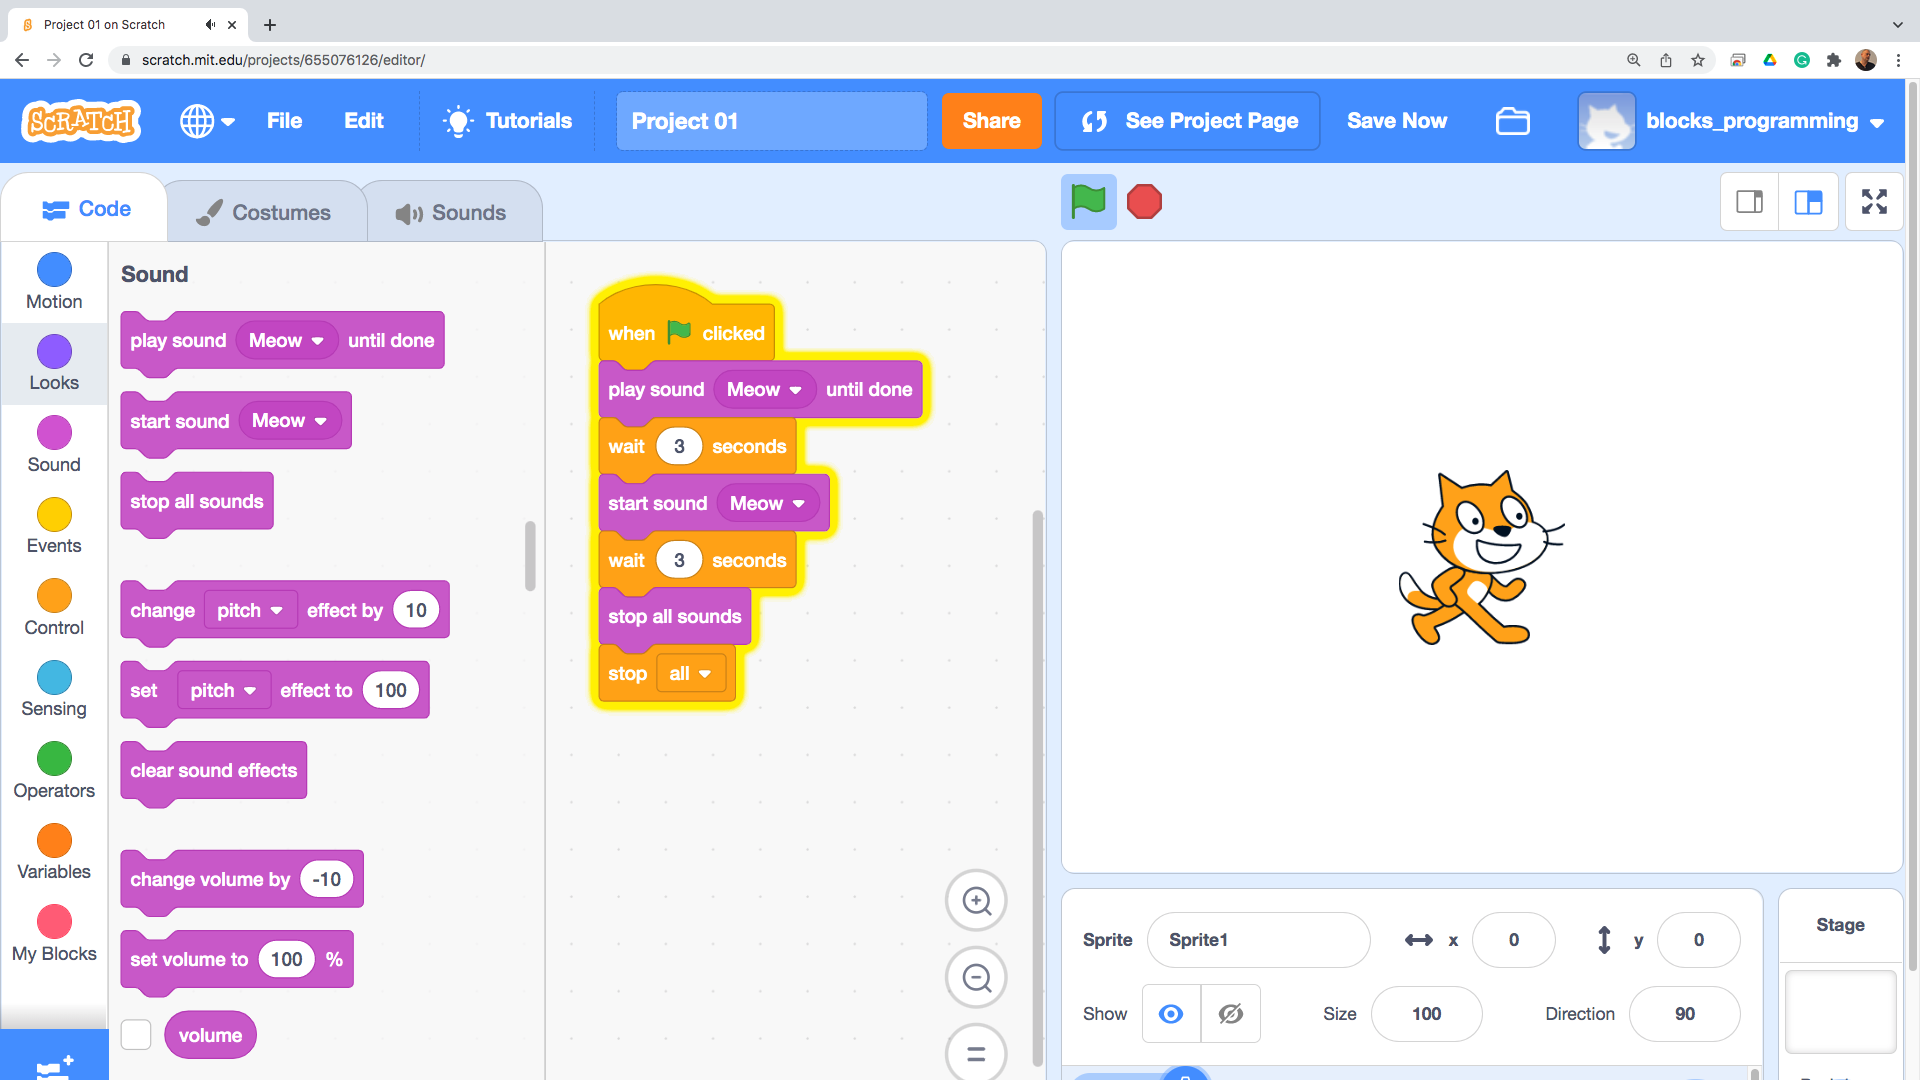
\includegraphics[width=1.0\linewidth,height=0.5\linewidth]{fig0076.png}
  \caption{Изпълнение на звуци}
\label{fig0076}
\end{figure}

Две от характеристиките на звуците могат да се променят с блокчетата за височина (честотна) и стерео озвучаване (ляво/дясно). И двете блокчета имат числени стойности за посочените характеристики (Фиг. \ref{fig0077}).

\begin{figure}[H]
  \centering
  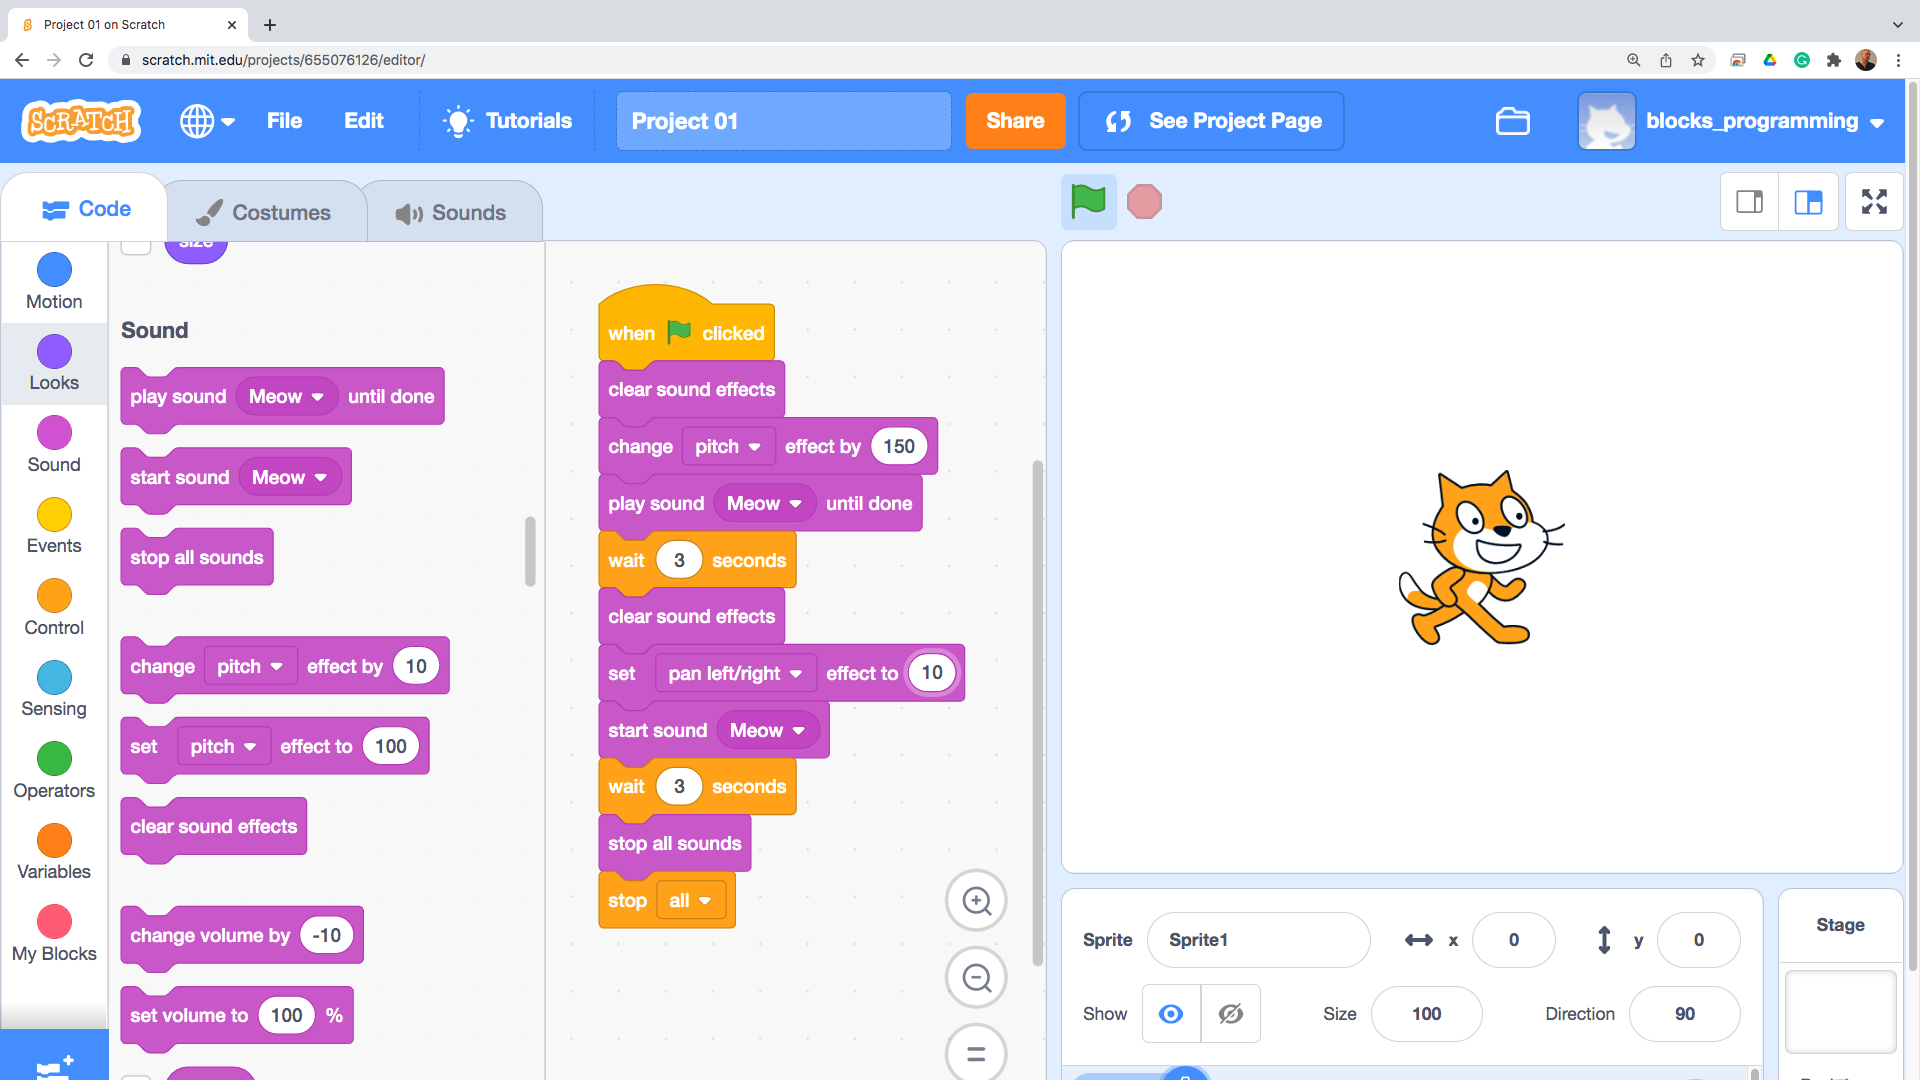
\includegraphics[width=1.0\linewidth,height=0.5\linewidth]{fig0077.png}
  \caption{Характеристики на звука}
\label{fig0077}
\end{figure}

За постигането на една по-богата звукова картина, силата на различните звуци може да се управлява с две блокчета (Фиг. \ref{fig0078}). Първото контролира силата на звука по абсолютна стойност, а второто като проценти. 

\begin{figure}[H]
  \centering
  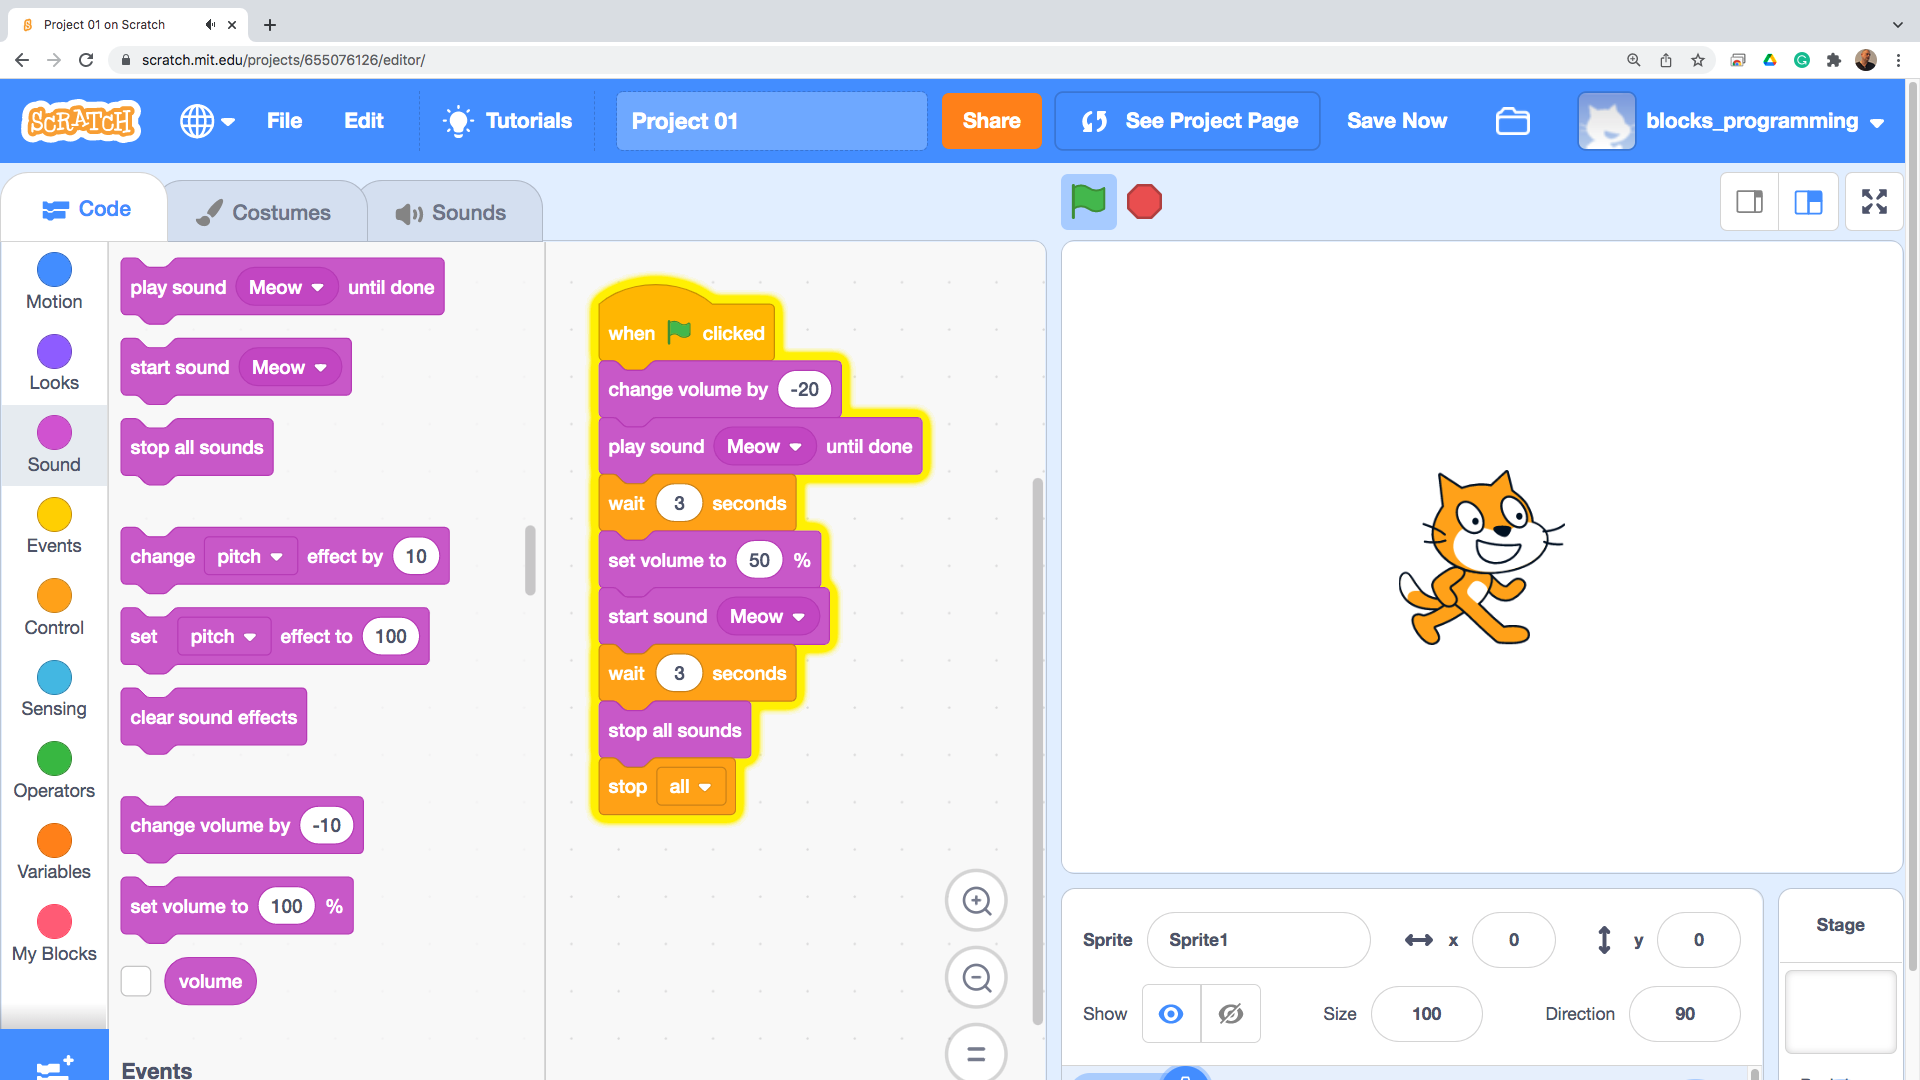
\includegraphics[width=1.0\linewidth,height=0.5\linewidth]{fig0078.png}
  \caption{Сила на звука}
\label{fig0078}
\end{figure}

Оранжевата група блокчета са предназначени за възникване на събития. Събитията са инструмент за изпълнение на инструкции, когато няма ясна престава за момента в който програмните инструкции трябва да се изпълнят. Такова събитие е натискане на бутон по клавиатурата от страна на потребителя (Фиг. \ref{fig0079}).

\begin{figure}[H]
  \centering
  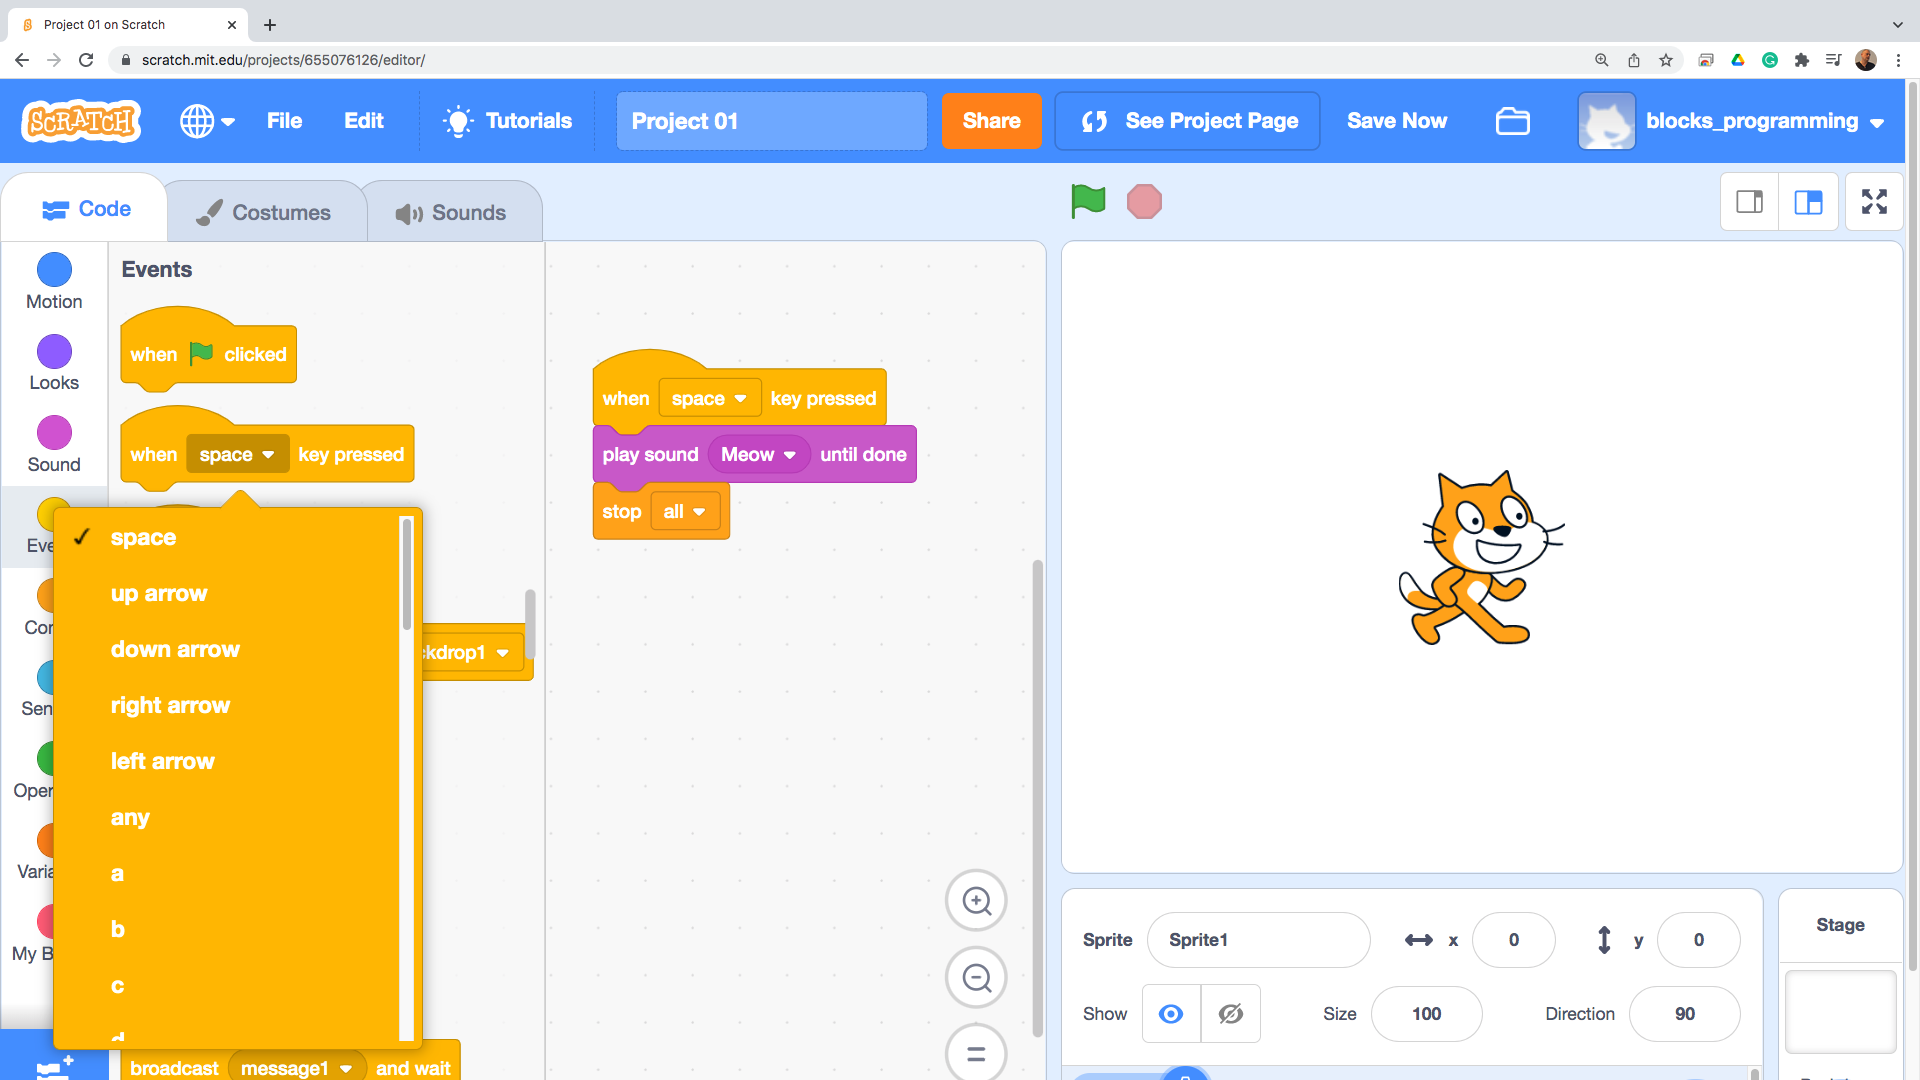
\includegraphics[width=1.0\linewidth,height=0.5\linewidth]{fig0079.png}
  \caption{Събитие за натискане на клавиш}
\label{fig0079}
\end{figure}

Кликването с мишката върху определен спрайт също може да бъде обработено с помощта на подходящо блокче (Фиг. \ref{fig0080}).

\begin{figure}[H]
  \centering
  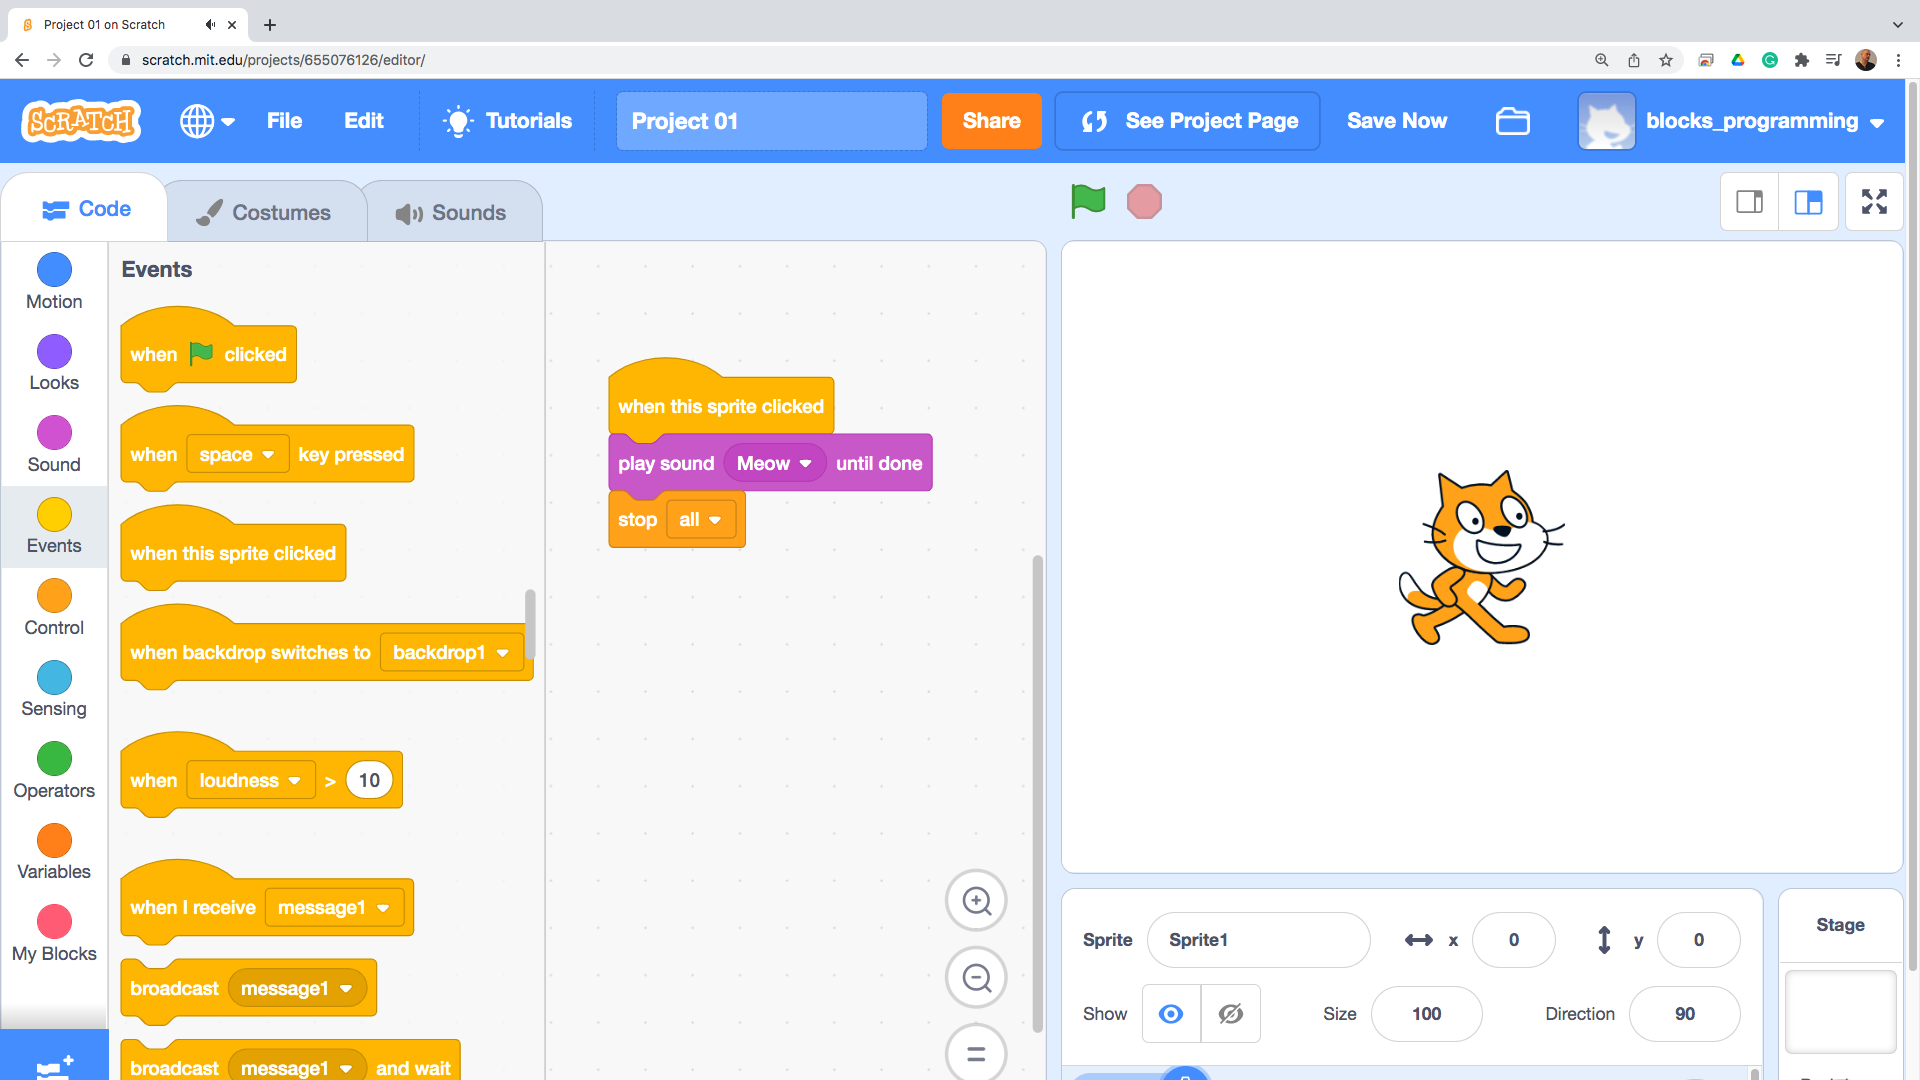
\includegraphics[width=1.0\linewidth,height=0.5\linewidth]{fig0080.png}
  \caption{Събитие за кликане с мишката}
\label{fig0080}
\end{figure}

Смяната на фона също може да предизвика обработване на събитие. За тази цел има предвидено блокче (Фиг. \ref{fig0081}).

\begin{figure}[H]
  \centering
  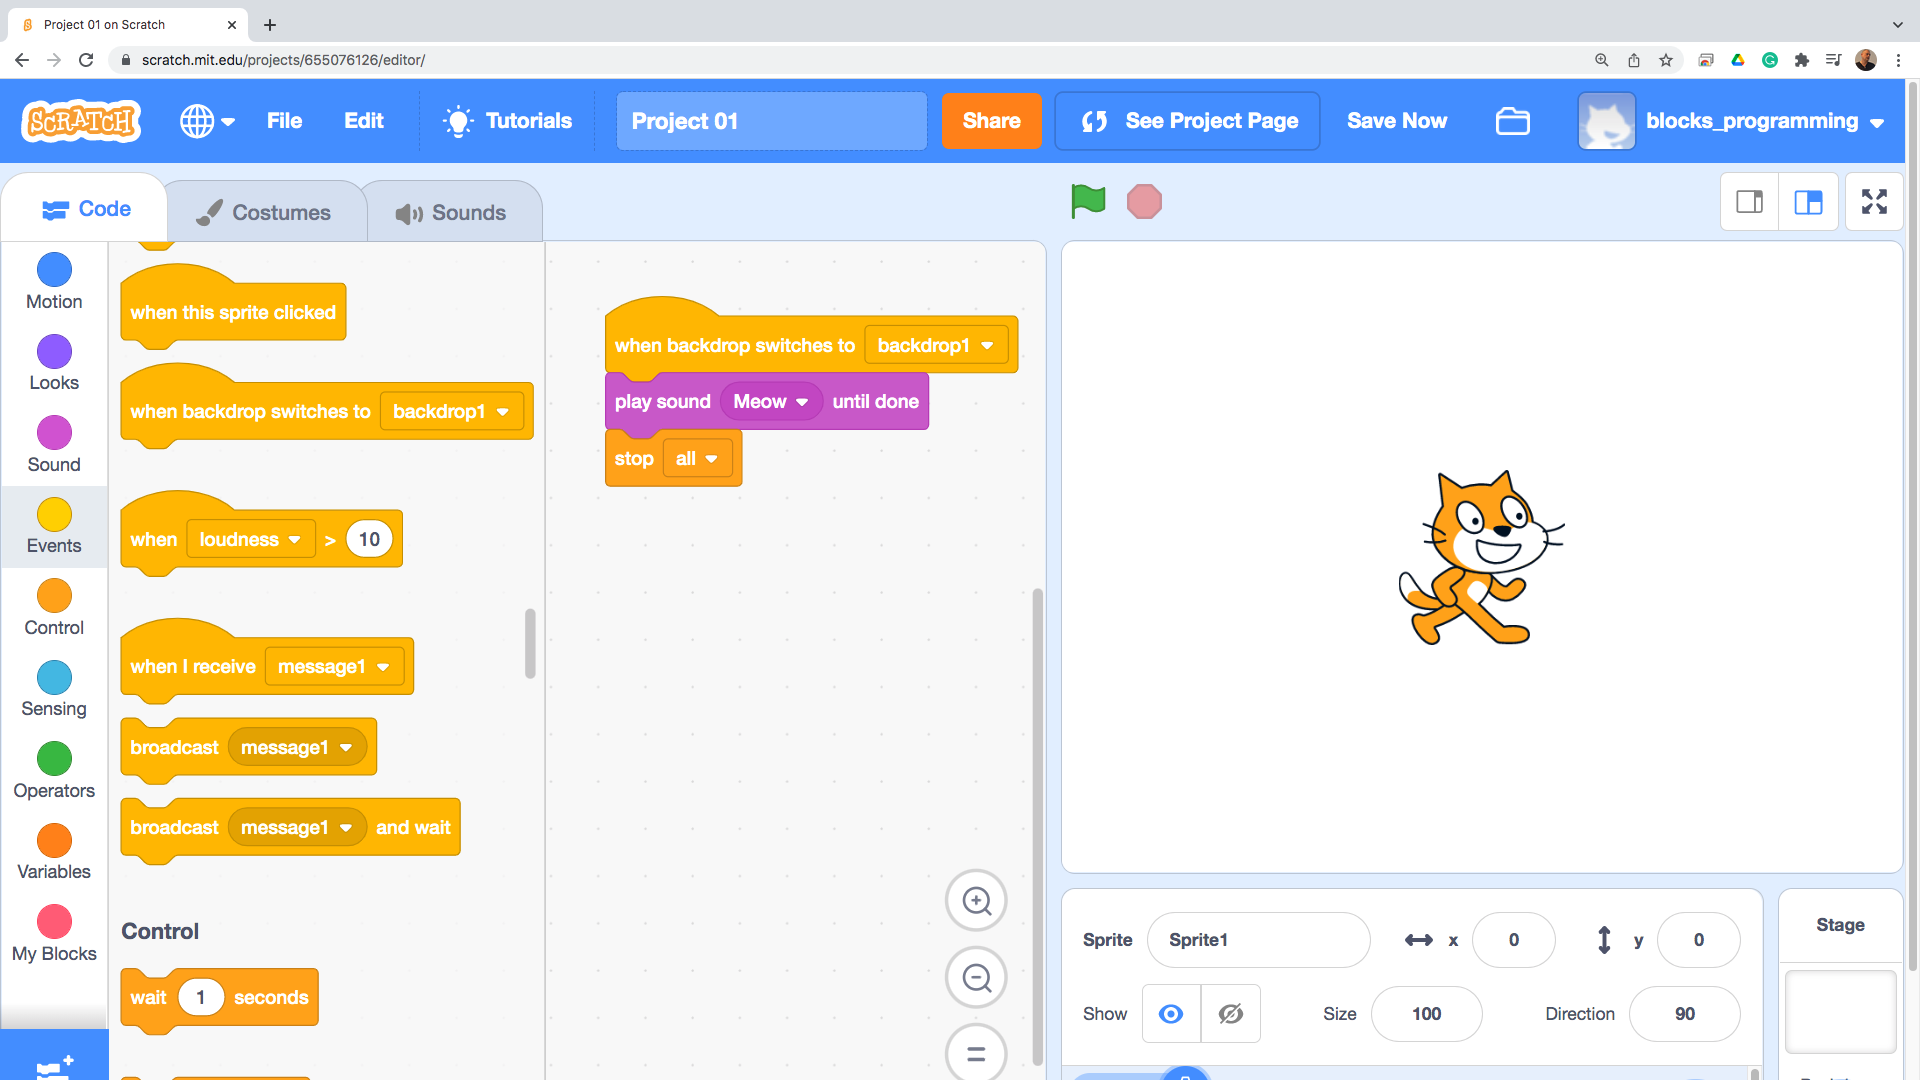
\includegraphics[width=1.0\linewidth,height=0.5\linewidth]{fig0081.png}
  \caption{Събитие за смяна на фона}
\label{fig0081}
\end{figure}

Събитие може да бъде прихванато след изтичане на определено време към таймер или достигане на определено ниво на звук (Фиг. \ref{fig0082}).

\begin{figure}[H]
  \centering
  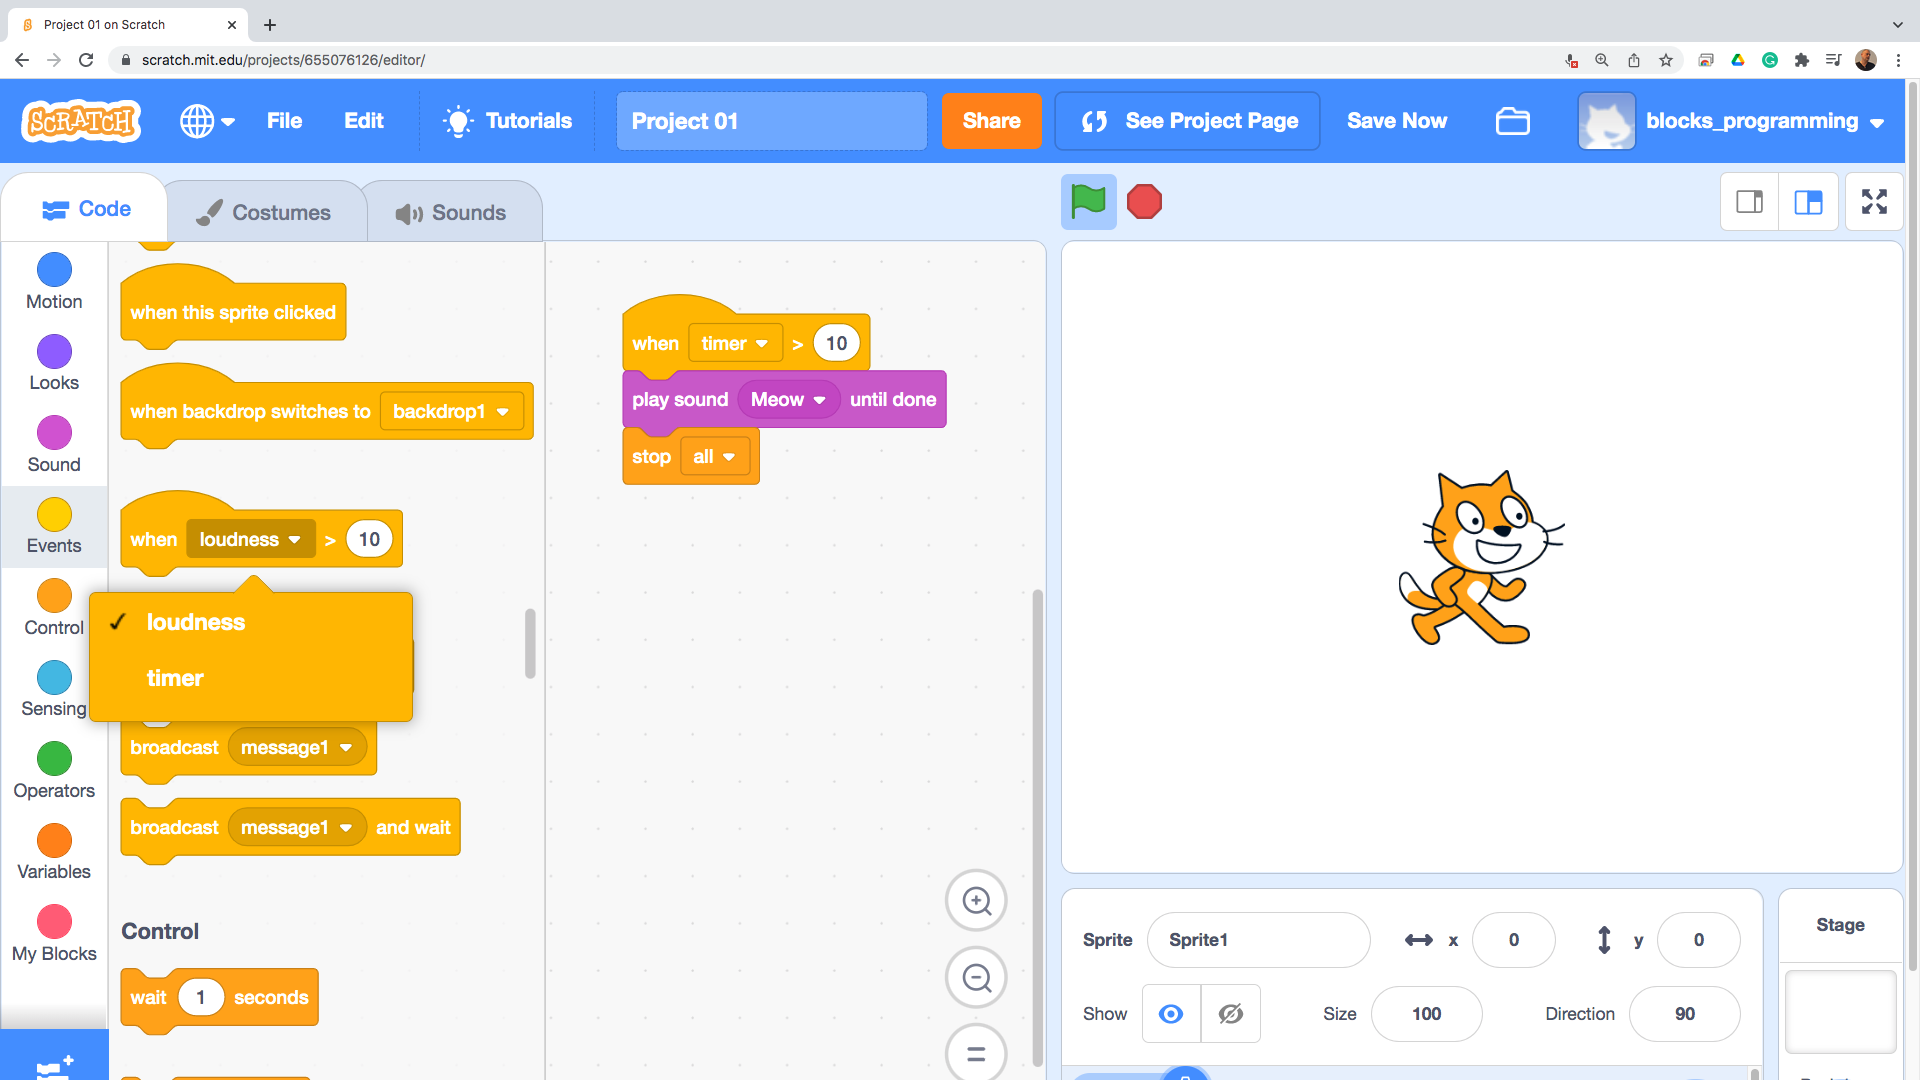
\includegraphics[width=1.0\linewidth,height=0.5\linewidth]{fig0082.png}
  \caption{Събитие от таймер или звук}
\label{fig0082}
\end{figure}

Работата със събития е свързана и с механизъм за предаване/получаване на съобщения. Един блок инструкции може да разпространи предварително дефинирано съобщение, а друг блок инструкции може да се абонира за получаването на точно този вид съобщение (Фиг. \ref{fig0083}).

\begin{figure}[H]
  \centering
  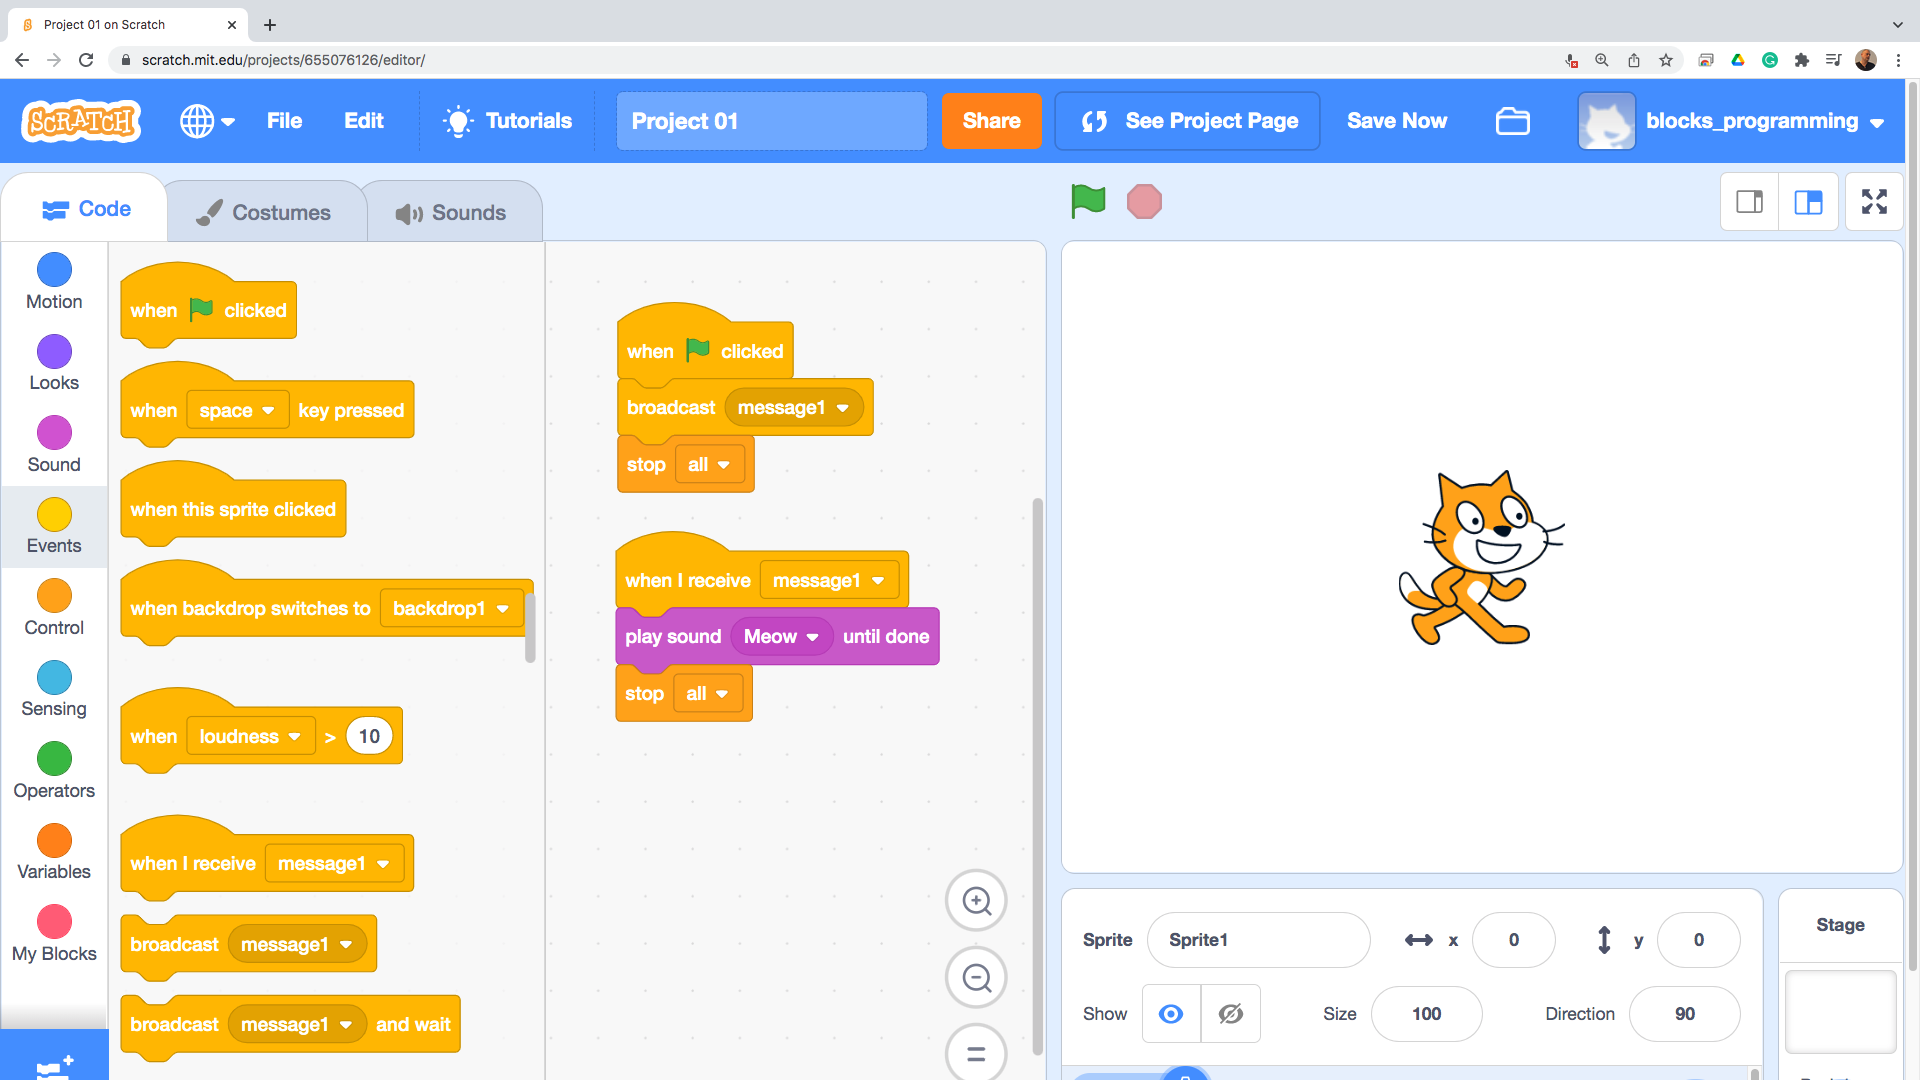
\includegraphics[width=1.0\linewidth,height=0.5\linewidth]{fig0083.png}
  \caption{Разпространяване и получаване на съобщения}
\label{fig0083}
\end{figure}

Тъй като работата с механизма за съобщения може да изисква синхронизация, то има отделно блокче, което разпространява съобщението и изчаква извършването на действията от прихващането му (Фиг. \ref{fig0084}). Програмистът може да създава различни съобщения, които да бъдат изпращани в различни ситуации. 

\begin{figure}[H]
  \centering
  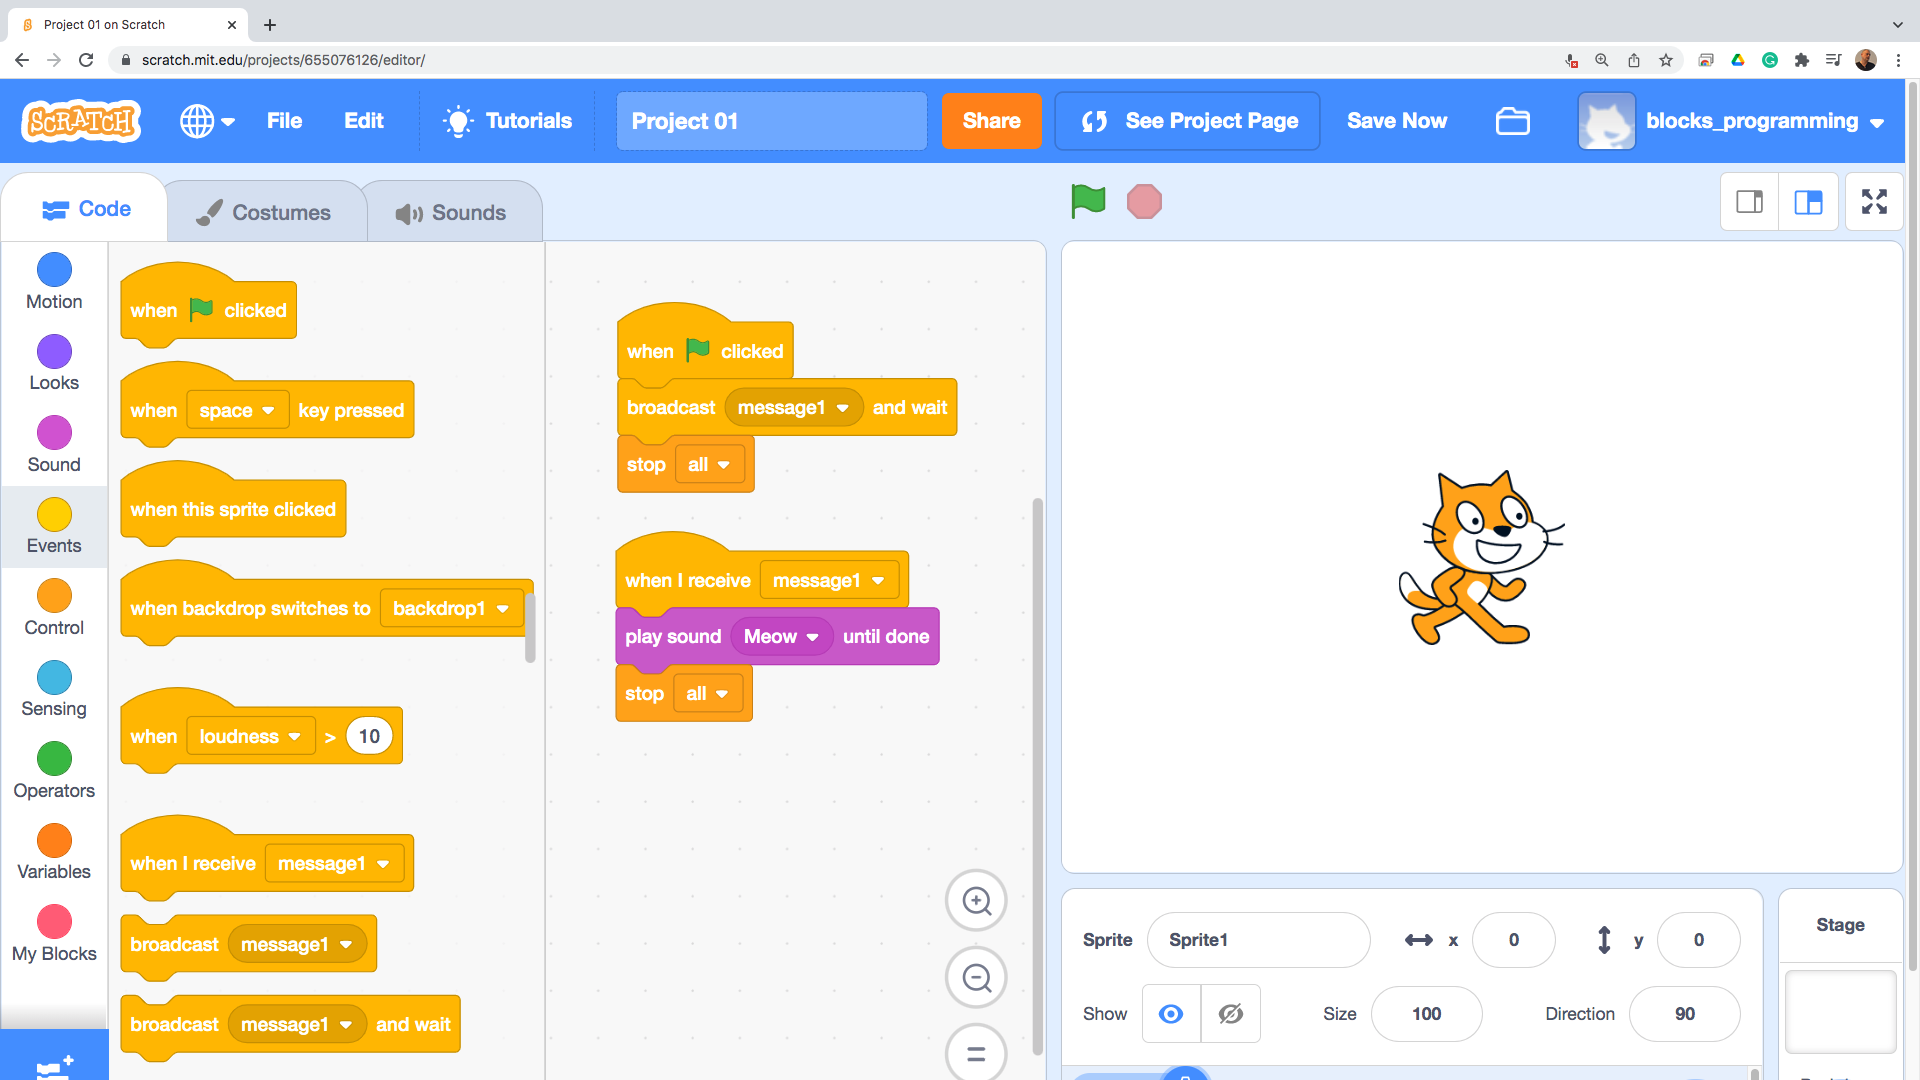
\includegraphics[width=1.0\linewidth,height=0.5\linewidth]{fig0084.png}
  \caption{Разпространяване на съобщение с изчакване}
\label{fig0084}
\end{figure}



